%% FEUP dissertation -- IDRISK2  (feupteses.sty)
%% Converted from the Word manuscript.

\documentclass[11pt,a4paper]{report}

\usepackage[utf8]{inputenc}

%% Mestrado em Inteligencia Artificial. FEUP-only cover (generic feupteses).
%% Working/provisional version. For jury/final stages add [juri] or [final].
\usepackage{feupteses}
%\usepackage[juri]{feupteses}
%\usepackage[final]{feupteses}

%% Path to the figures directory
\graphicspath{{figures/}}

%% Bibliography database
\addbibresource{backmatter/bibliography.bib}

%%========================================
\begin{document}

%%----------------------------------------
%% Information about the work
%%----------------------------------------
\title{European Food Safety Authority - AI-Enhanced Digital Registration and Analysis System}
\author{Bianca Oliveira}

%% Degree shown on the cover (FEUP-only layout)
\degree{Mestrado em Inteligência Artificial}

\copyrightnotice{Bianca Oliveira, \the\year{}}

\supervisor{Supervisor}{Prof.\ Lu\'{i}s Paulo Reis}
\supervisor{Second Supervisor}{Prof.\textsuperscript{a}\ M\'{o}nica Faria}

%% Committee (uncomment/fill for the jury version)
%\committeetext{Approved in oral examination by the committee:}
%\committeemember{President}{Prof.\ $<$Name$>$}
%\committeemember{Examiner}{Prof.\ $<$Name$>$}
%\committeemember{Member}{Prof.\ $<$Name$>$}

%%----------------------------------------
%% Preliminary materials
%%----------------------------------------
\begin{Prolog}
  %% abstract.tex: Resumo (PT) e Abstract (EN)  [FEUP]
%%
\chapter*{Resumo}

O sistema FoodEx2 da Autoridade Europeia para a Segurança dos Alimentos (EFSA) é o referencial padronizado para descrever produtos alimentares na monitorização da segurança alimentar europeia, mas a atribuição de códigos FoodEx2 continua a ser uma tarefa manual e fortemente dependente de peritos, o que limita a capacidade de resposta das autoridades reguladoras. Esta dissertação apresenta o IDRISK2, um pipeline multimodal de ponta a ponta que classifica produtos alimentares em códigos FoodEx2 diretamente a partir de imagens reais de rótulos, combinando reconhecimento ótico de caracteres (OCR), um modelo visão-linguagem (VLM) e um componente de Geração Aumentada por Recuperação (RAG) avançada construído sobre a documentação oficial do FoodEx2.

O pipeline foi avaliado num conjunto de imagens de pratos portugueses e brasileiros e de produtos embalados, comparando três VLM intermutáveis (GPT-4o, Claude Sonnet 4.6 e LLaVA-NeXT-Mistral-7B) sob as mesmas etapas de OCR, recuperação e geração. O sistema completo atingiu 29,4\% de correspondência exata e 58,8\% ao nível da família com o GPT-4o, tendo uma ablação confirmado que a camada de RAG avançada, e não o VLM isolado, produz praticamente todo o sinal de classificação útil. Os VLM proprietários tiveram desempenho semelhante e superaram claramente o modelo de código aberto. Uma análise de calibração revelou ainda que as saídas de elevada confiança estavam frequentemente incorretas e que o mecanismo automático de revisão humana detetou apenas uma pequena fração dos erros, indicando que a calibração da confiança é o principal obstáculo a uma implementação segura.

As principais contribuições são: um pipeline completo de imagem para FoodEx2 sobre rótulos reais; a primeira comparação empírica de VLM para classificação FoodEx2; um desenho de implementação fechado e atento à regulação; e uma caracterização honesta da lacuna de calibração que o trabalho futuro deverá colmatar.

\vspace{\fill}
\begin{flushleft}
{\Large \textbf{Palavras-chave}:}
FoodEx2 \(\bullet\)
Modelos Visão-Linguagem \(\bullet\)
Geração Aumentada por Recuperação \(\bullet\)
OCR \(\bullet\)
Segurança Alimentar \(\bullet\)
Calibração de Confiança
\end{flushleft}
\vspace*{24mm}

\acresetall

\chapter*{Abstract}

The European Food Safety Authority's FoodEx2 system is the standardised framework for describing food products in European food-safety monitoring, yet assigning FoodEx2 codes remains a manual, expertise-intensive task that limits the throughput of regulatory authorities. This dissertation presents IDRISK2, an end-to-end multimodal pipeline that classifies food products into FoodEx2 codes directly from real product-label images and combines optical character recognition (OCR), a vision-language model (VLM), and an Advanced Retrieval-Augmented Generation (RAG) component built over the official FoodEx2 documentation.

The pipeline was evaluated on an image dataset of Portuguese and Brazilian dishes and packaged products, comparing three interchangeable VLM backends (GPT-4o, Claude Sonnet 4.6, and LLaVA-NeXT-Mistral-7B) under identical OCR, retrieval, and generation stages. The full system reached 29.4\% exact-match and 58.8\% family-level accuracy with GPT-4o, with an ablation confirming that the Advanced RAG layer, rather than the VLM alone, produces essentially all of the usable classification signal. The proprietary VLMs performed comparably and clearly outperformed the open-source model. A calibration analysis further revealed that high-confidence outputs were frequently incorrect and that the automatic human-review trigger surfaced only a small fraction of errors, indicating that confidence calibration is the key obstacle to safe deployment.

The main contributions are: a complete image-to-FoodEx2 pipeline operating on real labels; the first empirical comparison of VLMs for FoodEx2 classification; a closed, regulation-aware deployment design; and an honest characterisation of the calibration gap that future work must close.

\vspace{\fill}
\begin{flushleft}
{\Large \textbf{Keywords}:}
FoodEx2 \(\bullet\)
Vision-Language Models \(\bullet\)
Retrieval-Augmented Generation \(\bullet\)
OCR \(\bullet\)
Food Safety \(\bullet\)
Confidence Calibration
\end{flushleft}
\vspace*{24mm}

\acresetall
   % Resumo (PT) + Abstract (EN)
%  \include{frontmatter/un-sdg}    % UN Sustainable Development Goals (optional)
  \chapter*{Acknowledgements}
%\addcontentsline{toc}{chapter}{Acknowledgements}

Aos meus orientadores, o Professor Luís Paulo Reis e a Professora Mónica Faria, agradeço por contribuírem para o meu crescimento ao longo desta dissertação.

Agradeço também a todos os meus colegas e superiores da VirtualCare, pelo apoio e pelas condições que tornaram possível a conclusão deste projeto.

Aos meus amigos, obrigada por estarem sempre presentes durante toda esta trajetória e por serem a minha família longe de casa.

Ao Guthemberg Ferreira, agradeço a parceria de sempre. Esteve ao meu lado em cada etapa da execução deste trabalho, dividindo comigo as dificuldades e as conquistas.

À minha mãe e ao meu pai, às minhas tias, irmãs e primas, agradeço por, mesmo à distância, terem me dado apoio incondicional, incentivo e amor para me sustentar em cada passo desta caminhada.

Por fim, e mais importante do que tudo, aos meus avós, Elci e Deuza Simões, o meu agradecimento mais profundo por serem a minha base. Por sempre terem investido e se doado em prol da minha educação, por me incentivarem em cada momento e por me ajudarem a me tornar a pessoa que sou hoje. Ao meu avô, por ter me incentivado desde sempre a cultivar o hábito da leitura; à minha avó, por tantas vezes ter se doado para me levar e me trazer da escola, do cursinho e de tudo o que eu precisasse. Amo muito vocês.

\vspace{10mm}
\begin{flushleft}
Bianca Oliveira
\end{flushleft}
    % acknowledgements
  \chapter*{Declaração de Honra}
%\chapter*{Declaration of honour}

Declaro que a presente dissertação é de minha autoria e não foi previamente
apresentada e avaliada nesta ou em outra instituição.
As referências a outros autores (afirmações, ideias, pensamentos),
assim como a utilização de trabalhos publicados respeitam escrupulosamente
as regras da atribuição, e encontram-se devidamente indicadas no texto e
nas referências bibliográficas, de acordo com as normas de referenciação.
Tenho consciência de que a prática de plágio ou de autoplágio constituem
ilícitos académicos, conforme estabelecido no Código de Ética da U.Porto.

Declaro, ainda, que utilizei ferramentas de Inteligência Artificial para a
realização de parte(s) da presente dissertação, e essa utilização e os seus
resultados estão devidamente assinalados e foram objeto de cuidada
verificação para deteção de erros, imprecisões, atribuições infundadas
ou outras formas de enviesamento de conteúdos e argumentos, bem como
de determinação de autoria.

\begin{flushleft}
\vskip 4\baselineskip
Bianca Oliveira
\vskip 3\baselineskip
%% linha para assinatura à mão
\rule{0.6\linewidth}{0.2mm}
\end{flushleft}
     % declaration of honour
%  \include{frontmatter/quote}     % optional epigraph
  \cleardoublepage
  \pdfbookmark[0]{Table of Contents}{contents}
  \tableofcontents
  \cleardoublepage
  \pdfbookmark[0]{List of Figures}{figures}
  \listoffigures
  \cleardoublepage
  \pdfbookmark[0]{List of Tables}{tables}
  \listoftables
  \chapter*{List of Acronyms and Abbreviations}
\chaptermark{LIST OF ACRONYMS}

\begin{longtable}{@{}p{0.20\textwidth}p{0.74\textwidth}@{}}
\toprule
\textbf{Acronym} & \textbf{Meaning}\\
\midrule
\endhead
AI & Artificial Intelligence\\
API & Application Programming Interface\\
ASAE & Autoridade de Segurança Alimentar e Económica (Portugal)\\
BAAI & Beijing Academy of Artificial Intelligence (developer of the bge-m3 embedding model)\\
BERT & Bidirectional Encoder Representations from Transformers\\
BLEU & Bilingual Evaluation Understudy\\
BM25 & Best Matching 25 (lexical ranking function)\\
CER & Character Error Rate\\
CLAHE & Contrast Limited Adaptive Histogram Equalisation\\
CLIP & Contrastive Language-Image Pre-training\\
CNN & Convolutional Neural Network\\
ColBERT & Contextualised Late Interaction over BERT (cross-encoder reranker)\\
EFSA & European Food Safety Authority\\
EU AI Act & Regulation (EU) 2024/1689, European Union Artificial Intelligence Act\\
EXIF & Exchangeable Image File Format\\
FAISS & Facebook AI Similarity Search (vector index library)\\
FEAST & FoodEx2-Enhanced Adaptive Scalable Taxonomy (Molfetta et al., 2025)\\
FoodEx2 & EFSA Food Classification and Description System (Revision 2)\\
FVST & Fødevarestyrelsen (Danish Veterinary and Food Administration)\\
GDPR & General Data Protection Regulation\\
GPT & Generative Pre-trained Transformer\\
HEIC / HEIF & High Efficiency Image Container / High Efficiency Image File Format\\
HMAC & Hash-based Message Authentication Code\\
HyDE & Hypothetical Document Embedding\\
IDRISK2 & AI-Enhanced Digital Registration and Analysis System for FoodEx2 (this work)\\
JSON & JavaScript Object Notation\\
LIMS & Laboratory Information Management System\\
LLM & Large Language Model\\
LSTM & Long Short-Term Memory\\
MRR & Mean Reciprocal Rank\\
NLP & Natural Language Processing\\
OCR & Optical Character Recognition\\
OEM & OCR Engine Mode (Tesseract parameter)\\
PDF & Portable Document Format\\
PSM & Page Segmentation Mode (Tesseract parameter)\\
RAG & Retrieval-Augmented Generation\\
RAGAS & Retrieval-Augmented Generation Assessment\\
RBAC & Role-Based Access Control\\
ROUGE & Recall-Oriented Understudy for Gisting Evaluation\\
RRF & Reciprocal Rank Fusion\\
SCA & Smart Coding Application (EFSA tool)\\
SHA-256 & Secure Hash Algorithm (256-bit output)\\
SIT & Servizio Igiene e Tossicologia (Italy)\\
SSO & Single Sign-On\\
SWRL & Semantic Web Rule Language\\
VLM & Vision-Language Model\\
WER & Word Error Rate\\
XLSX & Office Open XML Spreadsheet (Microsoft Excel format)\\
\bottomrule
\end{longtable}
    % list of acronyms
\end{Prolog}

%%----------------------------------------
%% Body
%%----------------------------------------
\StartBody

\hypertarget{introduction}{%
\chapter{Introduction}\label{introduction}}

This chapter provides an overview of the IDRISK2 project, including its motivation, objectives, and the overarching problem it aims to solve within the context of European food safety regulations and data management.

\hypertarget{context-and-problem-statement}{%
\section{Context and Problem Statement}\label{context-and-problem-statement}}

Food security represents a critical challenge, with significant implications for public health, economic stability, and societal well-being, particularly in the context of increasingly complex and globalised food supply chains. This complexity is further exacerbated by emerging food safety hazards stemming from factors such as climate change, novel materials in agri-food systems, and evolving dietary trends, necessitating advanced systems for their identification, assessment, and management \parencite{john_f__leslie_d22f2c65}.

For this reason, the European Food Safety Authority (EFSA) has developed standardised frameworks such as FoodEx2 to classify and describe food products consistently, which is fundamental for effective food safety risk assessment \parencite{hern_n_g__redondo_919f3cec}. FoodEx2 is a hierarchical system that represents food items using base terms and facets, which add further information about the food items.

Within the FoodEx2 hierarchy, three main types of terms are defined: hierarchy terms (aggregated groups), core terms (representing the minimum level of detail for coding), and extended terms (providing additional detail beyond core terms) ((EFSA), 2015). In practice, food coding primarily relies on core and extended terms, collectively referred to as base terms. To further enhance the level of specificity, FoodEx2 incorporates facets, which describe additional characteristics of food items, such as origin, processing methods, physical state, and other relevant attributes. Additionally, some terms include implicit facets that are not explicitly codified but are inherently understood from the base term itself, such as those related to the source facet and the part-nature facet ((EFSA), 2015).

The FoodEx2 represents a significant advancement in food classification and monitoring, enabling the standardised representation of food items through a harmonised coding scheme. Nevertheless, the manual mapping of food descriptions to FoodEx2 codes remains a time-consuming and error-prone process, often leading to inconsistencies in data reporting. This laborious manual classification not only hinders efficient data analysis but also complicates the comparison of food consumption data across diverse sources, ultimately impacting the accuracy of food safety risk predictions (Eftimov et al., 2017).

The inherent complexity of manually classifying vast quantities of diverse food data according to the intricate FoodEx2 hierarchy often leads to inconsistencies, delayed regulatory responses, and significant operational costs for food safety authorities and industry stakeholders. In this context, recent advances in artificial intelligence have spurred the development of innovative solutions aimed at improving the efficiency and accuracy of food classification. Nevertheless, a persistent methodological debate remains regarding the optimal approach for hierarchical classification within multi-dimensional taxonomies, specifically, the choice between fine-tuning versus retrieval-augmented strategies for mapping natural language inputs \parencite{lorenzo_molfetta_f41ce012}.

Moreover, despite this progress, AI models continue to encounter significant limitations, particularly when interpreting complex multimodal data while simultaneously ensuring adherence to strict data privacy regulations, such as the General Data Protection Regulation. These challenges underscore the necessity for further research into developing AI-enhanced systems tailored specifically for FoodEx2.

Beyond these challenges, advanced AI models are susceptible to hallucinations, a phenomenon characterised by the generation of plausible yet factually incorrect or fabricated information, particularly in tasks that require accurate factual knowledge and contextual understanding. This vulnerability is particularly concerning in regulatory environments where the precision of automated risk assessment directly impacts public health outcomes \parencite{omer_faruk_sari_c479eead}. Furthermore, these models often require extensive training periods, which may limit their applicability in dynamic environments where continuous updates are necessary. This limitation is particularly relevant in the food domain, as the FoodEx2 classification system undergoes periodic updates, thus requiring adaptable and robust AI architectures.

\hypertarget{motivation}{%
\section{Motivation}\label{motivation}}

Motivated by the challenges in food classification, the IDRISK2 project addresses a critical bottleneck by proposing an AI-enhanced digital registration and analysis system designed to automate and streamline the process of FoodEx2 compliance. This system aims to improve data quality and facilitate more accurate risk assessments. Furthermore, it seeks to promote greater harmonisation of data collected by EFSA, contributing to more reliable and consistent food safety analyses.

Beyond its regulatory impact, this project also addresses operational challenges, where the automation of food classification can significantly reduce the time and manual effort required from inspectors, increasing efficiency and reducing inconsistencies. In this context, IDRISK2 aims to optimise the workflow of the registration and analysis process, enabling resources to be allocated more strategically and proactively in risk detection activities.

Additionally, the project contributes to technological innovation by exploring new use cases of artificial intelligence in food safety, combining Optical Character Recognition (OCR), Computer Vision, Vision-Language Models (VLMs), and Retrieval-Augmented Generation (RAG). The integration of these technologies enables digital registration systems to interpret and classify complex multimodal data more autonomously and accurately, improving the reliability of food classification processes.

Finally, this research aims to provide scientific contributions by advancing the understanding of the applicability of multimodal AI models and RAG approaches in complex regulatory environments. This includes evaluating their capabilities and limitations in interpreting documents and images for compliance with standards such as FoodEx2. Furthermore, this study adopts a more nuanced perspective on the regulatory challenges posed by the EU AI Act, recognizing that compliance requires going beyond simple log registration to address complex issues of risk classification and transparency \parencite{idse_lucien_val_e2ea81c6}. By fostering critical discussion on these requirements, this research contributes to the development of future, more robust approaches in food safety systems.

\hypertarget{research-questions}{%
\section{Research Questions}\label{research-questions}}

Based on the challenges and motivations identified in the previous sections, the following central research question is proposed.

How can the integration of Artificial Intelligence techniques, combining computer vision, Optical Character Recognition, and large language models enhanced with Retrieval-Augmented Generation, improve the efficiency, accuracy, and security of the FoodEx2 coding process in digital food sample registration, ensuring compliance with EFSA standards and relevant regulatory cybersecurity requirements for food safety systems?

\hypertarget{research-objectives}{%
\section{Research Objectives}\label{research-objectives}}

To address the central research question, this dissertation aims to develop and evaluate an AI-driven system for automated FoodEx2 classification, ensuring compliance with EFSA standards and regulatory requirements.

To achieve this goal, the following specific objectives are defined:

\begin{itemize}
\item
  Design a multimodal architecture integrating Optical Character Recognition (OCR), Computer Vision, and Large Language Models for food data interpretation
\item
  Develop a Retrieval-Augmented Generation (RAG) pipeline to support reliable and explainable FoodEx2 classification
\item
  Ensure compliance with GDPR and cybersecurity requirements for secure data processing
\item
  Evaluate the system performance using classification metrics such as accuracy, precision, recall, and processing time
\item
  Compare the proposed approach with baseline methods, including manual classification and non-RAG AI approaches
\item
  Assess the system's scalability and adaptability to evolving FoodEx2 standards
\end{itemize}

\hypertarget{scope-and-limitations}{%
\section{Scope and Limitations}\label{scope-and-limitations}}

Based on the motivations and objectives outlined, the scope of this research is limited to the development and evaluation of an AI-enhanced system tailored for FoodEx2 compliance within the context of digital food sample registration. This includes the classification of food items and ingredients according to the hierarchical structure of FoodEx2, incorporating both base terms and facets, while prioritizing the secure handling of multimodal data.

Additionally, this research includes the development of a digital registration workflow that supports data capture at the point of sampling and the generation of structured FoodEx2 outputs. The evaluation will consider classification performance and usability within simulated or controlled scenarios aligned with regulatory workflows.

The proposed system focuses on the use of artificial intelligence techniques to automate the interpretation of textual and visual information associated with food samples. This includes the extraction of textual information from product labels using Optical Character Recognition and the analysis of visual characteristics through Computer Vision techniques. Furthermore, the system explores the integration of Large Language Models with a Retrieval-Augmented Generation framework to enhance classification accuracy, explainability, and regulatory compliance.

Moreover, the scope includes the development of a secure, closed AI model environment, ensuring data privacy and regulatory compliance by avoiding reliance on public cloud solutions or external unverified APIs. The system architecture will prioritize adherence to GDPR and other relevant cybersecurity protocols, ensuring robust data protection throughout the registration and analysis pipeline. However, it is important to note that, as a research prototype, this system focuses on foundational security and privacy principles rather than claiming full certification or compliance with the complex "high-risk" obligations stipulated by the EU AI Act (cf. Val, 2025 \parencite{idse_lucien_val_e2ea81c6}).

However, this research acknowledges certain limitations. The inherent complexity and continuous evolution of the FoodEx2 taxonomy may require ongoing model retraining and adaptation, which fall outside the scope of this dissertation. Additionally, the proposed system will be developed as a research prototype and may not include full integration with existing regulatory infrastructures such as EFSA or LIMS systems. Furthermore, the evaluation will be conducted using selected datasets and scenarios, which may not fully represent the diversity of real-world food products and operational conditions.
  % Introduction
\hypertarget{background-and-fundamentals}{%
\chapter{Background and Fundamentals}\label{background-and-fundamentals}}

This section provides a foundational understanding of the key theoretical concepts and technologies underpinning the proposed AI-enhanced system, encompassing food classification principles, artificial intelligence methodologies, and relevant regulatory frameworks. Specifically, it will delineate the structural components and terminologies of the FoodEx2 classification system (2.1), foundational concepts in artificial intelligence such as optical character recognition and computer vision techniques (2.2), and the pertinent regulatory landscape including GDPR provisions for data privacy and security (2.4).

\hypertarget{foodex2-classification-system}{%
\section{FoodEx2 Classification System}\label{foodex2-classification-system}}

The food domain plays a fundamental role in society, with far-reaching impacts across multiple sectors, including public health, economic stability, and environmental sustainability. Given this broad societal influence, ensuring the safety, quality, and traceability of food products has become increasingly important. These challenges highlight the need for effective monitoring and control mechanisms in food production and distribution, which are often overseen by regulatory authorities such as the European Food Safety Authority (EFSA). In response, EFSA developed the FoodEx2 Classification System, a standardised framework designed to harmonise food classification and support consistent food safety risk assessment \parencite{hern_n_g__redondo_919f3cec}.

Building on the terminology introduced in Section 1.1, the taxonomy is organised in two complementary structural dimensions. The first is the base-term hierarchy, which spans broad food groups (for example, A001A "Live animals"), intermediate sub-groups, and species-level or preparation-level distinctions, with each term identified by a unique code following the structural format of an A-prefix followed by four alphanumeric characters. The taxonomy comprises 31,303 approved terms and 298 deprecated terms organised across five complementary views, hierarchy, reporting, exposure, ingredient, and pesticide, each tailored to a specific regulatory use case ((EFSA), 2015). The second dimension is the facet system, which decomposes the description of a food item into orthogonal characterisation axes, source, part-nature, processing methods, physical state, packaging, and others, each providing a controlled vocabulary that can be combined with the base term to capture compositions or processing variants that do not warrant a dedicated base term of their own. The taxonomy is distributed in two complementary formats: the technical documentation describing the system's governance and use, and the Appendix B XLSX export containing the full set of approved terms with their associated metadata.

Similar to the food domain itself, FoodEx2 is a system that is continuously evolving and improving. In addition to the document The food classification and description system FoodEx2 (Revision 2), which provides guidance for the harmonised use of the system and quality control of FoodEx2 codes, EFSA publishes periodic updates that introduce modifications and new terms. Furthermore, EFSA provides several supporting tools, such as the Catalogue Browser and the Smart Coding Application (SCA), which facilitate code search and support the practical use of the FoodEx2 classification system \parencite{pedro_nabais_3f3d64d2,marina_nikoli__22bc7ee3}.

The system plays a crucial role in harmonising data collection for food consumption and chemical occurrence, enabling robust exposure assessments across Europe \parencite{marina_nikoli__c1230f7a,magalie_weber_debfa18b}. Therefore, the importance of FoodEx2 extends beyond its role as a classification system, functioning as a key tool for communication, data standardisation, and research. However, its inherent complexity and continuous evolution make manual application challenging, highlighting the need for innovative and automated solutions.

\hypertarget{artificial-intelligence-in-data-processing}{%
\section{Artificial Intelligence in Data Processing}\label{artificial-intelligence-in-data-processing}}

Artificial intelligence has emerged as a key technology for processing complex and large-scale datasets, particularly in domains that require the integration of heterogeneous data sources, such as food safety and regulatory compliance \parencite{rawan_elragal_fb5fd9d1}. The increasing availability of digital data, including images, textual descriptions, and structured metadata, has enabled the development of AI-driven systems capable of automating data interpretation and classification tasks.

This section reviews the core AI technologies underpinning the proposed system. It begins with Optical Character Recognition as the text extraction layer for image-based sources such as product labels. It then examines computer vision techniques that support the identification of visual features beyond text, followed by Large Language Models, which enable semantic interpretation of product information and regulatory documents. The integration of both visual and linguistic modalities is addressed through Vision-Language Models. Finally, given that AI models can generate inaccurate or fabricated outputs, particularly in specialised domains with incomplete data, Retrieval-Augmented Generation framework is introduced as the mechanism to ground the model's responses in external, up-to-date knowledge bases, thereby enhancing factual accuracy and reducing the propensity for generating fallacious information \parencite{zahra_namkhah_66f512ba}.

\hypertarget{optical-character-recognition-ocr}{%
\subsection{Optical Character Recognition (OCR)}\label{optical-character-recognition-ocr}}

Optical Character Recognition is a specialised application of computer vision that converts different types of documents, such as scanned paper documents, PDFs, or images captured by a digital camera, into editable and searchable data \parencite{do_hee_kim_9624c3df}. This technology enables the transformation of unstructured visual information into machine-encoded text, supporting better processing and analysis of the information.

An OCR system typically involves several stages, including image preprocessing, character recognition, and post-processing, each contributing to the accuracy and efficiency of text extraction. Modern OCR engines, such as Tesseract, have significantly advanced beyond basic digitisation to become core components of intelligent data capture systems, often integrating with AI and machine learning techniques for sophisticated information extraction and Intelligent Document Processing \parencite{munasprianto_ramli_8ac57418}.

At image preprocessing, algorithms are applied to enhance image quality and isolate text regions, often involving steps like binarisation, noise reduction, and skew correction to optimise character recognition accuracy. Following this, character recognition engines utilise advanced machine learning algorithms, including deep convolutional and recurrent neural networks, to accurately identify and translate these isolated textual elements into digital text, even amidst variations in font, size, and orientation \parencite{chih_chung_hsu_2d9c1cb7}. Finally, post-processing techniques employ linguistic models and dictionaries to correct recognition errors and ensure the output text is coherent and semantically accurate.

Despite these advancements, OCR technology struggles with challenging document layouts and low-quality images, significantly impacting its overall accuracy and reliability. As explored in the following section, advances in computer vision offer promising solutions to these limitations.

\hypertarget{computer-vision-techniques}{%
\subsection{Computer Vision Techniques}\label{computer-vision-techniques}}

Computer vision, a field of artificial intelligence, enables machines to interpret and understand visual information from the real world, analogous to human sight. This discipline involves developing algorithms and models that allow computers to process, analyse, and make decisions based on images and videos, transforming raw pixel data into meaningful insights. This capability is crucial for tasks such as object recognition, scene understanding, and motion analysis, which are vital for automated systems interacting with physical environments. In the context of the IDRISK2 project, computer vision is pivotal for analyzing multimodal data, specifically for extracting salient visual features from images of food products and packaging, which directly informs FoodEx2 compliance assessments.

Key computer vision techniques include image segmentation, which partitions an image into multiple segments to simplify analysis, and feature extraction, which identifies and describes unique attributes within an image for tasks like object detection and recognition. A foundational architecture enabling these capabilities is the Convolutional Neural Network (CNN), which processes images through successive layers of learned filters that progressively extract hierarchical visual representations, from low-level edges and textures to high-level semantic features such as product type or packaging format (Sadeghi-Tehran et al., 2019). These properties make CNNs particularly well-suited for tasks such as food product classification and ingredient identification from label images. These capabilities are directly applicable to the OCR pipeline described in Section 2.2.1, where text detection and recognition in high-resolution label images benefit significantly from convolutional feature extraction \parencite{renqing_luo_2e752c97}.

However, current vision encoder models still face limitations in simultaneously supporting both image and text recognition with human-like proficiency, especially when interpreting textual information embedded within complex document layouts such as tables, graphs, and mixed media (Zhu et al., 2024). This presents a significant challenge and demands the use of specialised multimodal learning approaches that can effectively integrate visual and linguistic cues to overcome these interpretation gaps. As explored in the following sections, the integration of vision encoders with Large Language Models, forming what are known as Vision-Language Models, represents a promising direction to address these limitations in the context of automated FoodEx2 classification.

\hypertarget{large-language-models-llms}{%
\subsection{Large Language Models (LLMs)}\label{large-language-models-llms}}

Large Language Models are advanced neural network architectures, typically transformers, trained on vast corpora of text data to understand, generate, and process human language with remarkable fluency and coherence.

These models excel at tasks such as text generation, summarisation, translation, and question answering, exhibiting an emergent capacity for complex reasoning and knowledge representation. Their architectural design, characterised by self-attention mechanisms, enables them to weigh the importance of different words in an input sequence, thereby capturing long-range dependencies crucial for contextual understanding. This capability allows LLMs to discern nuanced semantic relationships and infer contextual meaning from extensive textual inputs, making them highly effective for tasks requiring deep linguistic analysis.

A common approach to enhancing their utility involves tokenising input sequences according to a predefined vocabulary and predicting the distribution of probabilities for the next token's occurrence, predominantly employing Transformer architecture \parencite{yuki_imajuku_f8c4877b}. While encoder-only models are adept at capturing document-specific information, and encoder-decoder models handle variable-length and multimodal inputs, recent decoder-only Large Language Models have demonstrated promising performance in understanding and generating document content by leveraging diverse multimodal datasets including image segmentation and layout information \parencite{weishi_wang_67b85d63}. This flexibility allows decoder-based LLMs to handle various text generation tasks, such as question answering and translation, without requiring specialised training or adjustments for each task (Zhang et al., 2024). Specifically, the evolution of language models, from statistical to neural, pre-trained, and ultimately large language models, reflects a progression towards more sophisticated context-aware representations and enhanced generative capabilities \parencite{pengfei_zhou_b2203b1e}.

In the context of multimodal AI systems, LLMs serve as a powerful semantic backbone, interpreting linguistic elements extracted from documents and integrating them with visual information to provide comprehensive analysis for tasks like food item classification and compliance verification \parencite{yutong_zhang_e47bed88,chaoyang_zhu_ed468d29}.

However, their general applicability often falters in specialised domains, where a lack of domain-specific training can lead to inaccuracies and ``hallucinations'' \parencite{mohbat_tharani_ccbd7a9f}. This limitation underscores the necessity for integrating LLMs with external knowledge sources, motivating the adoption of Retrieval-Augmented Generation, discussed in Section 2.3, as a complementary architecture to ground model outputs in the FoodEx2 knowledge base, thereby improving reliability and reducing spurious outputs.

\hypertarget{vision-language-models-vlms}{%
\subsection{Vision-Language Models (VLMs)}\label{vision-language-models-vlms}}

Vision-Language Models represent a class of multimodal architectures that jointly process visual and textual information, bridging the gap between computer vision and natural language understanding. These models extend the capabilities of traditional LLMs by incorporating image encoders and projection layers, allowing them to interpret visual data encoded into tokens that align with textual representations, thereby enabling comprehensive understanding of multimodal inputs \parencite{zhipei_xu_621e96fd}.

The core technical challenge in VLMs is the alignment of visual and linguistic representations into a shared semantic space, a process commonly referred to as cross-modal fusion. Three principal fusion strategies have been proposed in the literature. Early fusion integrates raw or low-level features from both modalities before any high-level processing, allowing the model to learn joint representations from the outset but requiring tightly coupled training data. Late fusion, by contrast, processes each modality independently through dedicated encoders and combines their outputs at the decision level, offering greater modularity but potentially losing fine-grained cross-modal interactions. Intermediate fusion, the dominant paradigm in contemporary VLMs, integrates modality-specific representations at intermediate layers through cross-modal attention mechanisms, enabling the model to selectively attend to relevant visual regions in response to linguistic queries or vice-versa \parencite{ye_jiang_6fce7e4a}. This is particularly powerful for document understanding tasks, where the spatial layout of visual elements carries semantic meaning, such as associating a product logo with its textual name, or linking the visual structure of a nutritional table to its encoded values.

In the context of the IDRISK2 project, VLMs are particularly suited to the challenge of interpreting food product labels and packaging, where relevant information is conveyed through a combination of images, typographic elements, and structured text. By integrating the visual feature extraction capabilities described in Section 2.2.2 with the semantic reasoning of LLMs outlined in Section 2.2.3, VLMs enable a more comprehensive analysis of multimodal inputs, going beyond what OCR alone can capture in terms of layout understanding and visual context. By processing these heterogeneous inputs jointly, VLMs generate a unified multimodal representation of each food product that serves as the basis for FoodEx2 classification, going beyond what any single modality could capture in terms of layout understanding, visual context, and linguistic reasoning.

However, VLMs still present limitations in specialised domains, particularly when precise and consistent classification is required. Their performance can be constrained by the quality and diversity of training data, and they may struggle to reliably adhere to structured taxonomies such as FoodEx2 without additional grounding mechanisms. This reinforces the need for a Retrieval-Augmented Generation framework, as discussed in Section 2.3, to complement VLM outputs with verified, domain-specific knowledge.

\hypertarget{retrieval-augmented-generation-rag}{%
\section{Retrieval-Augmented Generation (RAG)}\label{retrieval-augmented-generation-rag}}

Retrieval-Augmented Generation is an architectural framework that enhances the capabilities of generative language models by combining them with a dynamic retrieval mechanism over external knowledge sources. RAG systems retrieve relevant documents or excerpts from a knowledge base at the time of inference, providing the language model with an up-to-date, domain-specific context to guide its outputs \parencite{patrick_lewis_10d460b7,xiaoye_qu_52f808ee}. In the context of the IDRISK2 project, this framework is directly applicable: it allows classification decisions to be grounded in the official FoodEx2 documentation published by the European Food Safety Authority (EFSA), ensuring that the model outputs remain aligned with the established regulatory taxonomy.

\hypertarget{principles-of-rag}{%
\subsection{Principles of RAG}\label{principles-of-rag}}

The fundamental principle underlying RAG is the separation of parametric knowledge, embedded in model weights during training, from non-parametric knowledge, which is stored externally and retrieved on demand. This decoupling allows the system to remain factually accurate and current without requiring retraining, making it particularly well-suited for regulatory domains where taxonomies and guidelines are subject to periodic revisions \parencite{amin_haeri_1f9fd225}.

A standard RAG pipeline consists of three sequential phases: indexing, retrieval, and generation. During indexing, source documents are preprocessed, segmented into chunks, and encoded into dense vector representations using embedding models, which are then stored in a vector database for efficient similarity search. At inference time, the retrieval phase queries this index to identify the most semantically relevant passages given an input. Finally, in the generation phase, the retrieved passages are concatenated with the original query and provided as context to the language model, which produces a response grounded in both the retrieved information and its parametric knowledge \parencite{harsh_chaudhari_a38f87a0,nirmal_kumar_roy_0d477fb0}. This architecture effectively reduces hallucinations by constraining model outputs to verifiable, domain-specific content, while also improving the interpretability and auditability of the system's decisions.

A critical design decision in RAG systems is the chunking strategy, the method by which source documents are segmented prior to indexing. Fixed-size chunking divides documents into segments of a predetermined token length, offering simplicity and consistency but potentially fragmenting semantically coherent passages. Semantic chunking, by contrast, segments documents based on content boundaries such as sentences, paragraphs, or sections, preserving contextual integrity at the cost of variable chunk sizes (``Proceedings of the 19th Conference on Computer Science and Intelligence Systems (FedCSIS),'' 2024). For structured regulatory documents such as FoodEx2 technical guidelines, semantic chunking is particularly advantageous, as it ensures that hierarchical descriptor definitions and classification rules are not fragmented across multiple chunks, preserving the precision required for accurate retrieval.

The quality of retrieval is further determined by the embedding model used to encode both document chunks and input queries into a shared vector space. Embedding models such as those based on the Sentence-BERT architecture or more recent models such as text-embedding-ada-002 generate dense vector representations that capture semantic similarity beyond lexical overlap, enabling the retrieval of contextually relevant passages even when exact terminology differs \parencite{maria_flavia_lovin_0fb6ab18}. The resulting vectors are stored in purpose-built vector stores such as FAISS, Chroma, or Pinecone, which support efficient approximate nearest neighbour search at scale.

\hypertarget{rag-architectures}{%
\subsection{RAG Architectures}\label{rag-architectures}}

As the field has matured, three principal RAG architectural paradigms have emerged, each offering different trade-offs between simplicity, flexibility, and retrieval quality: naive RAG, advanced RAG, and modular RAG (Pipitone \& Alami, 2024; ``Proceedings of the 20th Conference on Computer Science and Intelligence Systems (FedCSIS),'' 2025).

Naive RAG follows the straightforward pipeline described above, indexing, retrieval, and generation, and represents the foundational approach. While effective for simple, well-structured knowledge bases, it is sensitive to retrieval quality and can produce suboptimal results when queries are ambiguous or when retrieved passages lack sufficient specificity for complex classification tasks. Furthermore, naive retrieval relies exclusively on a single similarity search pass, without any mechanism to refine or validate the relevance of retrieved content before generation \parencite{yuhe_ke_37be3f59}.

Advanced RAG addresses these limitations through the introduction of additional processing stages both before and after retrieval. Pre-retrieval techniques such as query rewriting, query expansion, and hypothetical document embeddings (HyDE) improve the alignment between the input query and the indexed content, compensating for vocabulary mismatches and semantic ambiguity \parencite{c__edwards_c148eac9,honglin_wan_dd61983a}. Post-retrieval enhancements, including re-ranking, filtering, and answer validation, further refine the retrieved document set to ensure maximal relevance and factual consistency with the generative model's output. These enhancements are particularly relevant for structured taxonomies such as FoodEx2, where subtle distinctions between food categories demand high retrieval precision and where a single misretrieved passage can propagate classification errors.

Modular RAG extends this paradigm further by decomposing the pipeline into interchangeable functional components, including specialised retrievers, rerankers, memory modules, fusion mechanisms, and routing layers, that can be composed and adapted to specific task requirements \parencite{he_lin_7c94f881,andrea_matarazzo_da58af1d,aditi_singh_80d83cb6}. This flexibility enables the system to dynamically select retrieval strategies based on query characteristics, incorporate iterative retrieval loops for multi-step reasoning, and integrate multiple knowledge sources simultaneously. While Modular RAG offers the greatest adaptability, it also introduces greater implementation complexity and requires careful orchestration of its constituent components.

A transversal dimension across all architectures is the choice of retrieval method. Sparse retrieval methods such as BM25 rely on lexical matching and term frequency statistics, offering computational efficiency and interpretability but limited ability to capture semantic relationships beyond exact matches \parencite{yunfan_gao_9386ae73}. Dense retrieval methods, by contrast, encode both queries and documents as continuous vector representations and retrieve based on semantic similarity, enabling more nuanced matching at the cost of higher computational overhead. Hybrid retrieval combines both approaches, typically through score fusion or reciprocal rank fusion, to leverage the complementary strengths of lexical precision and semantic generalisation, and has demonstrated superior performance across a range of domain-specific retrieval benchmarks \parencite{yunfan_gao_9386ae73,akshay_govind_srinivasan_fc4e560a}. This combined approach is particularly valuable in specialised fields where both precise keyword matching for rare entities and broad semantic understanding for complex concepts are critical, enhancing the overall robustness and accuracy of retrieval systems.

\hypertarget{evaluation-of-rag-systems}{%
\subsection{Evaluation of RAG Systems}\label{evaluation-of-rag-systems}}

Evaluating RAG systems presents unique challenges, as performance depends on the quality of both the retrieval and generation components, as well as their interaction. A comprehensive evaluation framework must therefore assess each stage independently as well as the end-to-end system performance \parencite{ioannis_papadimitriou_0c7acc17}.

At the retrieval level, standard information retrieval metrics such as Precision, Recall, and Mean Reciprocal Rank (MRR) measure the ability of the retriever to surface relevant passages given an input query. Context Precision quantifies the proportion of retrieved chunks that are genuinely relevant to the query, while Context Recall measures the extent to which all necessary information for a correct answer is present in the retrieved context \parencite{hao_yu_7fec6693}.

At the generation level, faithfulness measures whether the model's output is factually grounded in the retrieved context, penalising responses that introduce information not supported by the retrieved passages. Answer Relevance assesses the degree to which the generated response directly addresses the input query, independent of faithfulness. Together, faithfulness and answer relevance form the core metrics of frameworks such as RAGAS \parencite{andrew_brown_84e43c08}, which has emerged as a widely adopted standard for automated RAG evaluation. Additionally, automated metrics like BERTScore, BLEU, and ROUGE evaluate the linguistic quality and similarity of the generated text to human-written references, albeit with limitations in assessing factual accuracy or semantic nuance.

For domain-specific applications such as FoodEx2 classification, these general metrics must be complemented by task-specific evaluation criteria, including classification accuracy against ground truth FoodEx2 codes, consistency of outputs across semantically equivalent queries, and robustness to variations in input quality such as degraded OCR outputs or incomplete product descriptions. The definition of an appropriate evaluation protocol for the IDRISK2 system is discussed further in the Methodology chapter.

\hypertarget{data-privacy-and-security}{%
\section{Data Privacy and Security}\label{data-privacy-and-security}}

The development and deployment of AI-powered systems within regulatory environments necessitates careful consideration of data privacy and security frameworks. Even in contexts where personally identifiable information is not directly processed, systems operating within the European Union are subject to a comprehensive legislative landscape governing data handling, model accountability, and the ethical use of automated decision-making. In the context of the IDRISK2 project, adherence to these frameworks is essential not only for legal compliance but also for ensuring the trustworthiness and auditability of the classification pipeline.

\hypertarget{general-data-protection-regulation-gdpr}{%
\subsection{General Data Protection Regulation (GDPR)}\label{general-data-protection-regulation-gdpr}}

The General Data Protection Regulation, enforced since May 2018, establishes the primary legal framework governing data processing activities within the European Union and the European Economic Area, with extraterritorial reach impacting entities outside the EU that process data pertaining to EU citizens \parencite{salvatore_sapienza_0b06a4a0}. While its provisions are primarily directed at the protection of personal data, the GDPR introduces broader principles of data governance, including purpose limitation, data minimisation, and accountability, that are relevant to any AI system operating within EU jurisdiction, regardless of whether personal data is directly involved.

Of particular relevance to automated classification systems is Article 22 of the GDPR, which addresses automated decision-making and profiling. Systems that produce decisions with legal or similarly significant effects based solely on automated processing are subject to specific obligations, including the right to human oversight and the provision of meaningful explanations for automated decisions \parencite{tuan_d__pham_cd6a9823}. Although the IDRISK2 system processes product data rather than personal data, the principle of explainability embedded in the GDPR aligns with broader requirements for transparency and accountability in regulatory AI applications, reinforcing the importance of interpretable classification outputs.

Furthermore, the GDPR's principle of privacy by design mandates that data protection considerations be integrated into system architecture from the outset, rather than treated as an afterthought \parencite{jelena_schmidt_e77b64ec}. For the IDRISK2 system, this translates into ensuring that any product data ingested, processed, or stored during the classification pipeline is handled in accordance with the minimum necessary scope, with appropriate access controls and audit trails to support regulatory accountability.

\hypertarget{principles-of-secure-ai-models}{%
\subsection{Principles of Secure AI Models}\label{principles-of-secure-ai-models}}

Beyond legislative compliance, the security of AI models deployed in regulatory contexts requires attention to a distinct set of technical and organisational principles. AI systems that inform compliance decisions are attractive targets for adversarial manipulation, and their outputs must be robust, reproducible, and resistant to exploitation through adversarial attacks or data integrity breaches \parencite{dhruvitkumar_v__talati_5e1ce083}.

A foundational principle is model robustness, the capacity of the system to maintain accurate and consistent outputs when faced with noisy, incomplete, or adversarially perturbed inputs. In the context of the IDRISK2 system, this is particularly relevant given the variability of real-world food label images, which may present degraded text, inconsistent formatting, or partially occluded content. Robustness mechanisms, including input validation, confidence thresholding, and fallback procedures for low-quality inputs, are therefore integral to the system's security and trustworthiness, particularly when considering the potential for high-risk AI systems to impact health, safety, or fundamental rights \parencite{mateo_aboy_940b3b93}.

A further concern is data integrity, ensuring that the knowledge bases and regulatory documents used by the RAG pipeline are authentic, unaltered, and sourced from authoritative repositories such as the EFSA. Any corruption or unauthorised modification of the retrieval index could propagate errors into the classification outputs, with potential consequences for regulatory compliance. Secure ingestion pipelines, version control of indexed documents, and cryptographic verification of source integrity are therefore recommended practices for RAG-based systems operating in high-stakes domains \parencite{alex_dantart_273f7ed0,christoforus_yoga_haryanto_549a697c}.

Finally, the principle of transparency and auditability requires that the system's classification decisions be traceable and explainable to both technical and non-technical stakeholders. This aligns with the emerging EU AI Act framework, which classifies AI systems used in regulatory compliance contexts as high-risk, imposing obligations related to documentation, human oversight, and post-deployment monitoring \parencite{tomas_bueno_mom_ilovi__463b771a}. Designing the IDRISK2 system with these requirements in mind from the outset ensures that its deployment remains compliant with both current and anticipated regulatory obligations.
  % Background and Fundamentals
\hypertarget{literature-review}{%
\chapter{Literature Review}\label{literature-review}}

Building on the foundational concepts established in Chapter 2, this chapter critically examines existing research and implemented solutions at the intersection of food safety and artificial intelligence, focusing on the applications of these technologies, identified limitations, and existing gaps that the IDRISK2 system seeks to fill.

The review begins by surveying existing approaches to automated food data classification, from early rule-based systems to more recent machine learning methods (3.1). It then examines the application of AI techniques in food safety and traceability contexts, with particular attention to the use of OCR and computer vision (3.2.1) and large language models for food information extraction (3.2.2). The integration of multimodal AI for document processing is subsequently addressed (3.3), followed by a discussion of security and compliance considerations in AI deployments (3.4). The chapter concludes by identifying the key gaps in current research and technology that motivate the proposed approach (3.5).

\hypertarget{existing-systems-for-food-data-classification}{%
\section{Existing Systems for Food Data Classification}\label{existing-systems-for-food-data-classification}}

The use of automation represents a significant opportunity to improve the food data classification process, through successive generations of computational methods, each building upon the limitations of its predecessor. Early classification systems relied on predefined rules and structured ontologies to encode domain knowledge explicitly, offering transparency and alignment with established taxonomies but struggling to scale to the heterogeneity and ambiguity of real-world food data. The advent of machine learning introduced data-driven approaches capable of generalising across diverse inputs, progressively improving classification accuracy while reducing dependence on hand-crafted rules \parencite{_17165083__simon_pearson_76a456af,van_meer__floor_f66672e5}. However, the inherent complexity of hierarchical taxonomies such as FoodEx2, encompassing base terms, facets, and multilingual descriptors organised across multiple levels of specificity, has exposed the limitations of both paradigms, motivating the development of more sophisticated architectures integrating deep learning, natural language processing, and retrieval-based mechanisms.

This section reviews the principal approaches that have been proposed and evaluated in the literature, from rule-based and ontology-driven systems (3.1.1) to machine learning and neural methods (3.1.2), critically examining their contributions and limitations in the context of FoodEx2 compliance.

\hypertarget{rule-based-systems}{%
\subsection{Rule-Based Systems}\label{rule-based-systems}}

Before the proliferation of machine learning and deep learning approaches, rule-based systems were foundational in automating food data classification, relying on explicitly defined criteria and logical conditions to categorise food items \parencite{azanzi_jiomekong_ec1ddc5a}.

Ontology-based approaches represent an early form of this paradigm, encoding food knowledge through structured hierarchical vocabularies and logical relationships. FoodOn, for instance, leverages a comprehensive ontological framework to classify food products based on their source, processing, and composition, facilitating standardised data exchange and reasoning across diverse food-related datasets \parencite{gjorgjina_cenikj_0ae807f2,damion_dooley_8eedd589}.

At the information extraction level, rule-based named-entity recognition methods were among the first to be applied to food-related text. Eftimov et al. (2017) developed a rule-based Named Entity Recognition system for food information extraction from unstructured scientific literature demonstrating the viability of pattern-matching and linguistic rules for identifying food entities and related attributes (Eftimov et al., 2017).

A more applied instantiation of the rule-based paradigm is found in FoodWiki, an ontology-driven mobile system that uses semantic matching and SWRL inference rules to assess food product suitability based on consumer preferences and dietary restrictions \parencite{duygu__elik_ertu_rul_145c1b77}. While effective within its constrained domain, the system's reliance on a manually curated knowledge base limited its scalability and adaptability to new products or evolving food classifications.

Despite their utilities, these rule-based systems offer high precision when rules are meticulously crafted for specific domains, they inherently struggle with the variability and ambiguity present in diverse food descriptions, making them difficult to scale and maintain \parencite{simon_mezgec_ec31e9e4}. The brittleness of rule-based systems became increasingly apparent, motivating a shift towards data-driven machine learning approaches capable of learning classification patterns directly from examples.

\hypertarget{machine-learning-approaches}{%
\subsection{Machine Learning Approaches}\label{machine-learning-approaches}}

To increase the cognitive capacity of automatic food classification systems and overcome some limitations of rule-based systems, machine learning approaches have been increasingly employed, leveraging statistical models to identify complex patterns within large datasets for more flexible and scalable classification \parencite{n_n__misra_b6603190}.

Among the earliest semi-automated approaches specifically targeting FoodEx2 classification is StandFood, proposed by Eftimov et al. (2017), which combined a machine learning classifier for food category identification with a natural language processing module for FoodEx2 code assignment. Evaluated on datasets from three European countries, the system achieved an accuracy of 89\% for classification and 79\% for food description, establishing a foundational benchmark for subsequent work in the field. Despite its promising results, StandFood relied on shallow feature representations and predefined post-processing rules, limiting its capacity to generalise across the full depth and breadth of the FoodEx2 taxonomy.

Subsequent machine learning advancements, like the FoodEx2vec by \textcite{eftimov_foodex2vec_2020}, brought significant advances, introducing the first vector representation of food concepts within the FoodEx2 hierarchy. By embedding food items in a continuous hyperbolic space using Poincaré embedding, FoodEx2vec enabled the capture of hierarchical semantic relationships between food concepts, improving the alignment of multi-hierarchical data compared to traditional Euclidean methods \parencite{lorenzo_molfetta_47d7c4cd}. This work marked a transition towards neural and distributional approaches, demonstrating that the structural properties of the FoodEx2 taxonomy could be explored to enhance classification and food data analysis tasks.

The integration of deep learning and natural language processing into FoodEx2-compatible pipelines was further explored by \textcite{simon_mezgec_ec31e9e4}, who proposed a combined approach for food image recognition and standardisation, applying deep convolutional networks for visual classification and NLP-based matching for FoodEx2 code assignment. This work highlighted the potential of multimodal data fusion for comprehensive food item identification and classification within complex regulatory frameworks like FoodEx2.

The current state of the art in automated FoodEx2 classification is represented by FEAST \parencite{lorenzo_molfetta_47d7c4cd}, a retrieval-augmented multi-hierarchical food classification system specifically designed to address the challenges of complex label interdependencies, data sparsity, and extreme output dimensions inherent in the FoodEx2 system. The FEAST decomposes the classification task into three sequential stages: base term identification, multi-label facet prediction, and facet descriptor assignment, and employs a retriever-reranker architecture, achieving state-of-the-art accuracy by effectively navigating the multi-hierarchical structure of FoodEx2. Despite the noted limitations concerning data imbalance and coverage in the available datasets \parencite{lorenzo_molfetta_47d7c4cd}, FEAST's modular design offers both interpretability and scalability, allowing the retrieval index to be updated as new FoodEx2 codes emerge without requiring full model retraining.

However, despite these advances, a significant gap persists across the machine learning approaches reviewed. Most systems address classification from textual food descriptions alone, without integrating the visual and multimodal information present on real-world product labels. Furthermore, the absence of a publicly standardised benchmark dataset for FoodEx2 coding limits systematic comparison across approaches. Finally, none of the reviewed systems addresses the full pipeline from raw product image to compliant FoodEx2 output within a secure, regulation-aware deployment environment, a gap that the IDRISK2 project directly seeks to address.

\hypertarget{ai-applications-in-food-safety-and-traceability}{%
\section{AI Applications in Food Safety and Traceability}\label{ai-applications-in-food-safety-and-traceability}}

Beyond classification, the use cases for artificial intelligence in food safety and traceability are expanding rapidly, encompassing diverse applications such as risk prediction, supply chain optimisation, and pathogen detection \parencite{chenhao_qian_8525e6ba}. The increasing digitisation of food supply chains and the growing availability of multimodal data, including product images, nutritional labels, and regulatory documents, have created new opportunities for AI-driven automation across the food safety pipeline. This section delves into two of the most directly relevant application domains: the use of OCR and computer vision for automated information extraction from food product labels (3.2.1), and the application of large language models for semantic interpretation and compliance verification of food-related information (3.2.2).

\hypertarget{ocr-and-computer-vision-in-food-industry}{%
\subsection{OCR and Computer Vision in Food Industry}\label{ocr-and-computer-vision-in-food-industry}}

Optical Character Recognition and computer vision technologies are pivotal for automating the extraction and interpretation of textual and visual data from food product labels, packaging, and other physical documents within the food industry. This capability is crucial for enhancing food safety protocols and ensuring compliance with regulatory standards by enabling automated data capture from diverse sources \parencite{marina_arribas_lopez_6d42e82a}.

The automated extraction of information from food product labels represents one of the most practically significant applications of OCR and computer vision in the food industry. Product labels constitute the primary source of regulatory and nutritional information for both consumers and authorities, but their heterogeneity, encompassing varied fonts, multilingual text, dense layouts, and packaging materials that introduce glare and surface distortion, poses significant challenges for automated recognition systems \parencite{v_nia_guimar_es_e2e932db}.

Early approaches to label recognition relied on simple image processing techniques combined with traditional OCR engines such as Tesseract. Despite its widespread adoption, this technique struggles with the visual complexity characteristic of real-world food packaging. A comparative evaluation of four open-source OCR systems (Tesseract, EasyOCR, PaddleOCR, and TrOCR) on real-world food packaging images demonstrated significant performance variation across engines, without any system consistently outperforming others across all label types, highlighting the need for more robust, specialised solutions \parencite{mayimunah_nagayi_62f20413}. Hence, these findings underscore the importance of preprocessing pipelines tailored to the specific characteristics of food packaging, including binarisation, noise reduction, and perspective correction, to achieve optimal performance in automated information extraction from diverse food labels \parencite{mayimunah_nagayi_62f20413}.

More recent work has focused on the integration of vision-language models into OCR for food label recognition. \textcite{le_coffee_label_2025} proposed a framework combining advanced image enhancement with VLM-based OCR for coffee bean package label recognition, demonstrating that structured use of vision-language models can substantially improve text recognition accuracy on challenging packaging materials. Similarly, other studies have leveraged combined OCR and large language models to extract and analyse ingredients from food labels, offering insights into complex nutritional terms and providing risk assessments to consumers \parencite{sagar_janokar_7f0484cc}. This approach reflects a trend towards replacing traditional OCR engines with end-to-end vision-language pipelines capable of jointly performing text detection, recognition, and semantic interpretation in a single inference call.

Despite these advances, key limitations persist. Most systems are evaluated on constrained datasets that do not reflect the full diversity of commercial food products, and performance degrades significantly on low-resolution or occluded label images. Furthermore, OCR systems operating in isolation produce raw textual outputs that require subsequent semantic processing to be mapped to structured representations such as FoodEx2 codes, a gap that motivates the integration with large language models discussed in the following section.

\hypertarget{llms-for-food-information-extraction}{%
\subsection{LLMs for Food Information Extraction}\label{llms-for-food-information-extraction}}

In addition to extracting data from food images, the semantic interpretation of food-related information, including ingredient lists, nutritional data, and regulatory claims, represents a natural application domain for large language models, given their capacity for contextual understanding and flexible information extraction from heterogeneous textual sources. In contrast to rule-based and classical NLP approaches, LLMs do not require predefined extraction templates, enabling generalisation across diverse label formats and regulatory contexts \parencite{neris__zen_95877972}.

In the context of food safety compliance, \textcite{shabnam_hassani_c7097c31} demonstrated the applicability of LLMs (BERT and GPT-based models) to the automated classification of legal provisions and compliance verification in the food safety domain, including under GDPR constraints \parencite{shabnam_hassani_c7097c31}. The study concluded that LLMs are capable of reducing manual workload in regulatory analysis, though performance was sensitive to the specificity of the legal domain and the quality of prompting strategies \parencite{shabnam_hassani_c7097c31}.

Within the product label level, \textcite{fatmah_yousef_assiri_d1ac72fc} proposed a pipeline combining OCR with LLMs for the extraction of nutritional information from bilingual food labels, demonstrating that LLMs can effectively resolve the ambiguities and mismatch that commonly degrade the quality of raw OCR outputs \parencite{fatmah_yousef_assiri_d1ac72fc}. This work highlights the complementary relationship between OCR and LLMs in food label processing: the OCR provides the textual content while the LLMs provide the semantic layer required for structured information extraction \parencite{fatmah_yousef_assiri_d1ac72fc}.

Beyond individual labels, LLMs have also been evaluated for large-scale extraction of product information from online retail sources. A recent evaluation of LLM-based strategies for food product information extraction from German online shops demonstrated promising results for structured data extraction, with retrieval-augmented approaches outperforming standard prompting on tasks requiring precise attribute identification \parencite{brosch__christoph_34010501}. In the broader food safety domain, the integration of LLMs with knowledge graphs has emerged as a complementary paradigm, enabling the combination of structured domain knowledge with the flexible reasoning capabilities of generative models for risk prediction and traceability applications \parencite{mohbat_tharani_f8ffae09}.

However, LLMs applied to food information extraction are not without limitations. Their outputs remain susceptible to hallucinations in data-sparse or taxonomically complex scenarios, and their tendency to generate hallucinations is particularly problematic in regulatory contexts where precision is essential. These limitations reinforce the case for retrieval-augmented approaches that ground LLM outputs in verified knowledge bases, a direction examined in detail in Section 3.3.2.

\hypertarget{advancements-in-multimodal-ai-for-document-processing}{%
\section{Advancements in Multimodal AI for Document Processing}\label{advancements-in-multimodal-ai-for-document-processing}}

Given the inherent multimodal nature of food packaging (combining textual elements with visual cues like logos, brand imagery, and product photography), advancements in multimodal AI are particularly relevant for achieving robust and comprehensive information extraction \parencite{qingfeng_tian_6cb227c3,cheng_dong_zhang_6ced93cf}.

Therefore, this subchapter will explore the latest research in multimodal AI, specifically focusing on how the synergistic integration of visual and linguistic modalities can enhance the accuracy and completeness of data extraction from complex food-related documents. This section examines the state of the art in text-image fusion for document understanding (3.3.1) and the application of retrieval-augmented generation to domain-specific and regulatory contexts (3.3.2).

\hypertarget{state-of-the-art-in-text-image-fusion}{%
\subsection{State-of-the-Art in Text-Image Fusion}\label{state-of-the-art-in-text-image-fusion}}

The integration of textual and visual modalities for document understanding has evolved significantly over the past decade, progressing from shallow feature junction to deeply coupled architectures capable of cross-modal reasoning and semantic interpretation \parencite{shuaishuai_gao_50521934}. Early approaches often relied on concatenating features extracted independently from text (e.g., OCR output) and images (e.g., visual embeddings), subsequently feeding these combined representations into machine learning models for classification or extraction tasks. More recent advancements, however, emphasise unified multimodal representation frameworks that seamlessly integrate diverse data types to mitigate the limitations of isolated processing \parencite{lang_mei_8bcb958f}.

A foundational step towards deeper integration was the development of multimodal deep networks that jointly process document images and their OCR-extracted textual content through shared architectures. This approach showed that combining visual and textual features in a unified model consistently outperforms unimodal baselines on document classification benchmarks (...). Consequently, subsequent work extended this paradigm through attention-based fusion mechanisms, enabling models to dynamically weight the contribution of each modality based on the relevance of visual regions to the linguistic query, a property particularly valuable for structured documents where spatial organisation carries semantic meaning \parencite{paul_pu_liang_8415d006}.

The emergence of large-scale pre-trained vision-language models has further transformed the field. Contemporary architectures such as CLIP, LLaVA, and Qwen-VL leverage cross-modal attention and contrastive pre-training on massive image-text datasets to acquire generalisable multimodal representations that can be fine-tuned for downstream document understanding tasks \parencite{paul_pu_liang_8415d006}. A recent taxonomy of multimodal fusion approaches proposed by Li et al. categorises these methods based on their fusion strategy, ranging from early fusion where raw data is combined, to late fusion where decisions from unimodal models are merged, and hybrid approaches \parencite{abhinav_ramesh_kashyap_da0a8b8d}. More specifically, late fusion permits the use of specialised, established architectures for each modality, independently processing information until the final merging of predictions \parencite{thibault_douzon_fb62b0d4}.

Despite these advances, key challenges persist in the application of text-image fusion to regulatory document processing. Domain shift between general pre-training data and specialised regulatory documents remains a significant source of performance degradation, and the fine-grained classification requirements of structured taxonomies such as FoodEx2 demand precision levels that generalist multimodal models do not consistently achieve. These limitations motivate the integration of retrieval-augmented mechanisms, examined in the following section, as a complementary strategy to ground multimodal outputs in verified domain-specific knowledge.

\hypertarget{rag-based-solutions-in-scientific-domains}{%
\subsection{RAG-based Solutions in Scientific Domains}\label{rag-based-solutions-in-scientific-domains}}

The application of retrieval-augmented generation to regulatory domains has received considerable momentum as a strategy for addressing the limitations of language models alone, particularly concerning factual accuracy and domain specificity \parencite{monica_riedler_e70c1434}. By grounding model outputs in authoritative external documents retrieved at inference time, RAG systems offer a principled approach to combining the generative flexibility of large language models with the factual reliability of curated knowledge base \parencite{tuba_gokhan_1d9980e9}. This hybrid architecture directly mitigates issues such as hallucination and outdated information, which are critical considerations for compliance in frequently updated regulatory landscapes.

In the pharmaceutical and clinical domain, \textcite{waikar_rag_2026} evaluated RAG-based systems for reviewing the regulatory compliance of drug information and clinical trial protocols, demonstrating that integrated RAG/LLM pipelines substantially outperform standalone models on compliance verification tasks. This study highlighted the importance of retrieval precision, ensuring that the passages surfaced by the retriever are not merely topically related but specifically relevant to the regulatory requirement being evaluated, a challenge directly applicable to the FoodEx2 classification context, where nuances in product descriptions can significantly alter classification outcomes \parencite{hocine_kadi_3530c912,milad_moradi_83875958}.

Similar findings have been reported in the domain of technical regulatory interpretation. A RAG pipeline specifically designed for question answering over radio regulatory documents demonstrated that domain-specialised retrieval, grounded in authoritative regulatory corpora, significantly reduces hallucinations and improves response reliability compared to general-purpose LLMs operating without retrieval augmentation \parencite{kassimi__zakaria_el_f3c1dbe2}. The dense domain-specific vocabulary characteristic of regulatory documents, such as the structure of the FoodEx2 technical guidelines, was identified as a key factor motivating the RAG approach.

Within the food classification domain specifically, the FEAST system \parencite{lorenzo_molfetta_47d7c4cd} reviewed in Section 3.1.2, represents the most advanced application of retrieval-augmented architectures to FoodEx2 coding to date. Its modular design combining dense retrieval, cross-encoder reranking, and hierarchical classification, demonstrates the viability of RAG-based approaches for structured food taxonomy assignment and establishes a direct point of comparison for the pipeline proposed in this dissertation.

Therefore, it can be concluded that RAG-based architectures are suitable for regulatory compliance tasks characterised by structured knowledge bases, precise classification requirements, and the need for auditable and traceable outputs. However, existing implementations have largely operated only with textual inputs, without integrating the visual and multimodal information present in the labels of actual products, a gap that the IDRISK2 system directly addresses.

\hypertarget{security-and-compliance-in-ai-systems}{%
\section{Security and Compliance in AI Systems}\label{security-and-compliance-in-ai-systems}}

The deployment of AI systems in regulatory environments introduces a distinct set of security and compliance obligations that extend beyond technical performance considerations. As AI-driven pipelines increasingly inform decisions with regulatory or safety implications, ensuring that these systems operate within established legal frameworks has become a critical imperative. This section examines the compliance landscape defined by the GDPR and the EU AI Act (3.4.1), followed by a review of privacy-preserving AI techniques that operationalise these requirements at the architectural level (3.4.2).

\hypertarget{gdpr-compliance-in-ai}{%
\subsection{GDPR Compliance in AI}\label{gdpr-compliance-in-ai}}

The General Data Protection Regulation remains the primary legislative framework governing data processing activities within the European Union, and its provisions carry direct implications for AI systems that operate on or produce data pertaining to individuals or regulated entities. While the GDPR was not designed specifically for AI, its core principles have proven broadly applicable to AI system design, and their interpretation in the context of automated decision-making has been progressively clarified through regulatory guidance and judicial decisions \parencite{susan_von_struensee_ed47b0f9}.

Within the GDPR, Article 22 is particularly relevant for classification systems, as it restricts fully automated decision-making that produces significant legal or similar effects on individuals, establishing the right to human intervention and adequate explanation of automated results \parencite{andrew_d__selbst_b94e5789}. Although food product classification systems such as the IDRISK2 pipeline do not directly process personal data, the transparency and explainability obligations embedded in Article 22 establish a broader standard of accountability that applies to any AI system operating in a regulated context, reinforcing the importance of interpretable and auditable classification outputs.

The introduction of the EU AI Act (Regulation (EU) 2024/1689) has further expanded the compliance landscape for AI systems deployed within the EU. The Act establishes a risk-based regulatory framework that classifies AI systems according to their potential for harm, imposing stricter obligations on high-risk applications, including those used in regulatory compliance, critical infrastructure, and safety assessment contexts \parencite{enas_mohammed_alqodsi_071d9976}. Systems falling within the high-risk category are subject to requirements including mandatory risk management systems, technical documentation, human oversight mechanisms, and post-market monitoring, obligations that must be integrated into system design from the outset rather than retrofitted after deployment. The convergence of GDPR and AI Act requirements creates a layered compliance framework that AI developers in the food safety domain must navigate carefully, as non-compliance carries both legal and reputational risks.

\hypertarget{privacy-preserving-ai-techniques}{%
\subsection{Privacy-Preserving AI Techniques}\label{privacy-preserving-ai-techniques}}

Beyond legislative compliance, there is a growing focus on developing technical mechanisms that operationalise privacy protection at the architectural level of AI systems. Three principal paradigms have emerged as the dominant approaches: differential privacy, federated learning, and trusted execution environments, each addressing different threat models and privacy-utility trade-offs \parencite{zuzanna_fendor_276ddcba}.

Differential privacy provides formal mathematical guarantees of privacy by introducing calibrated noise into model training or inference processes, ensuring that the contribution of any individual data point cannot be reliably inferred from the model's outputs. This technique is particularly relevant for AI systems trained on sensitive datasets, as it bounds the information leakage attributable to any single training example while preserving aggregate statistical utility \parencite{reihaneh_torkzadehmahani_ed6428e5}. However, the noise injection required to achieve strong privacy guarantees can degrade model performance, particularly for fine-grained classification tasks, necessitating careful optimisation between privacy budget allocation and model utility for real-world deployment \parencite{ramit_sehgal_7100e259}.

Federated learning addresses privacy at the data collection level by enabling collaborative model training across distributed data sources without requiring raw data to be centralised. Each participating node trains a local model on its own data and shares only model updates, gradients or weights, with a central aggregator, thereby keeping sensitive data localised and reducing exposure to centralised data breaches \parencite{kilian_sprenkamp_729804de}. This paradigm is particularly attractive for regulatory AI applications involving multiple independent authorities or organisations, as it enables the development of shared models without requiring cross-institutional data sharing, a common constraint in food safety regulatory environments where data governance policies restrict data transfer.

Trusted execution environments provide hardware-level isolation for sensitive computation, ensuring that model inference and data processing occur within secure enclaves that are protected from the host operating system and external software. This approach is complementary to differential privacy and federated learning, providing an additional layer of protection against infrastructure-level threats such as memory inspection or malicious system administrators \parencite{haochen_liu_f33409d1}. The combination of these techniques is gaining traction as a standard approach for AI deployments in regulated, high-stakes domains where multiple threat vectors must be addressed simultaneously.

In the context of the IDRISK2 system, the relevance of these techniques is primarily architectural. The system's design prioritises a closed, self-hosted deployment environment that avoids reliance on public cloud infrastructure or external unverified APIs, thereby minimising data exposure risks at the infrastructure level. This design choice aligns with the principle of privacy by design mandated by the GDPR and provides a foundation for future integration of more advanced privacy-preserving techniques, should the scope expand to include distributed data sources or highly sensitive individual-level food consumption data.

\hypertarget{gaps-in-current-research-and-technology}{%
\section{Gaps in Current Research and Technology}\label{gaps-in-current-research-and-technology}}

Despite significant advancements in AI for food safety and compliance review, a set of persistent gaps remains. While significant progress has been made in individual components of automated food classification pipelines, no existing system has yet integrated these components into a unified, regulation-aware, multimodal architecture capable of end-to-end FoodEx2 compliance assessment from real-world product data.

\hypertarget{gap-1-no-end-to-end-pipeline-from-real-world-label-images-to-foodex2-output}{%
\subsubsection{Gap 1, No end-to-end pipeline from real-world label images to FoodEx2 output}\label{gap-1-no-end-to-end-pipeline-from-real-world-label-images-to-foodex2-output}}

The most significant gap in the current literature is the absence of a system capable of processing raw food product label images, as captured in real inspection conditions, and producing compliant FoodEx2 codes as output. FEAST \parencite{lorenzo_molfetta_47d7c4cd}, the most advanced existing approach, operates exclusively on pre-structured textual food descriptions and does not address the upstream challenge of extracting and interpreting the heterogeneous visual and textual content present on real packaging.

\hypertarget{gap-2-absence-of-vlm-evaluation-for-foodex2-classification}{%
\subsubsection{Gap 2, Absence of VLM evaluation for FoodEx2 classification}\label{gap-2-absence-of-vlm-evaluation-for-foodex2-classification}}

No existing work has systematically evaluated the applicability of Vision-Language Models to FoodEx2 classification from product label imagery. The growing capabilities of models such as GPT-4o, Claude, LLaVA, and Qwen-VL in document understanding and structured information extraction suggest significant potential for this task, yet no benchmark or comparative study exists.

\hypertarget{gap-3-regulatory-compliance-and-security-not-addressed-in-food-classification-ai}{%
\subsubsection{Gap 3, Regulatory compliance and security not addressed in food classification AI}\label{gap-3-regulatory-compliance-and-security-not-addressed-in-food-classification-ai}}

The reviewed literature on automated food classification devotes minimal attention to the regulatory and security dimensions of deployment in official food safety contexts. The specific implications of the GDPR and the EU AI Act for AI systems used in regulatory food safety workflows have not been systematically addressed in any existing food classification system.

\hypertarget{gap-4-absence-of-closed-self-hosted-deployment-architectures}{%
\subsubsection{Gap 4, Absence of closed, self-hosted deployment architectures}\label{gap-4-absence-of-closed-self-hosted-deployment-architectures}}

Existing AI-driven food classification systems predominantly rely on cloud-based infrastructure or external API services, introducing data governance risks incompatible with the strict requirements of official regulatory bodies such as ASAE, SIT, and FVST. The development of self-hosted, closed deployment architectures for food safety AI remains an underexplored area that the IDRISK2 project directly addresses.
  % Literature Review
\hypertarget{methodology}{%
\chapter{Methodology}\label{methodology}}

This chapter describes the design and implementation strategy of the IDRISK2 system, detailing the architectural decisions, component configurations, and integration mechanisms. The methodology is structured to address each of the research objectives defined in Section 1.4, progressing from data collection and preprocessing (section 4.2) through to the individual processing modules, their integration, and the security and compliance mechanisms governing the system's deployment.

\hypertarget{system-architecture-overview}{%
\section{System Architecture Overview}\label{system-architecture-overview}}

The IDRISK2 system is designed as a modular, end-to-end pipeline for automated FoodEx2 classification from multimodal food product data, as illustrated in Figure 4.1. The architecture integrates five principal layers that process the input sequentially from raw image to structured regulatory output.

The pipeline begins with an OCR and image processing module that extracts raw textual content from food product label images using one of three configurable engines (Tesseract, EasyOCR, or PaddleOCR) selected based on comparative evaluation described in Section 4.3. The extracted text and preprocessed image are subsequently passed jointly to a Vision-Language Model module, where one of three interchangeable candidate models (GPT-4o, Claude or LLaVA-NeXT) generates a unified multimodal representation of the product through cross-modal attention mechanisms.

This representation serves as the query input to the Advanced RAG pipeline, the central classification component of the system. The pipeline comprises three sequential stages: pre-retrieval enhancement through query rewriting and HyDE, hybrid retrieval combining dense semantic search with BM25 lexical matching via reciprocal rank fusion, and post-retrieval refinement through cross-encoder reranking and context compression. Retrieved passages are drawn from a Chroma vector store indexed over the official EFSA FoodEx2 documentation. The generation component then produces a structured FoodEx2 output, comprising a base term, applicable facets, a confidence score, and a traceable reference to the retrieved documentation.

All processing occurs within a security and compliance layer that enforces closed deployment, GDPR compliance mechanisms, and audit logging throughout the pipeline, contributing to the system's alignment with the regulatory obligations of the EU AI Act for high-risk AI applications, serving as a foundational component within broader compliance efforts.

\begin{figure}[htbp]
\centering
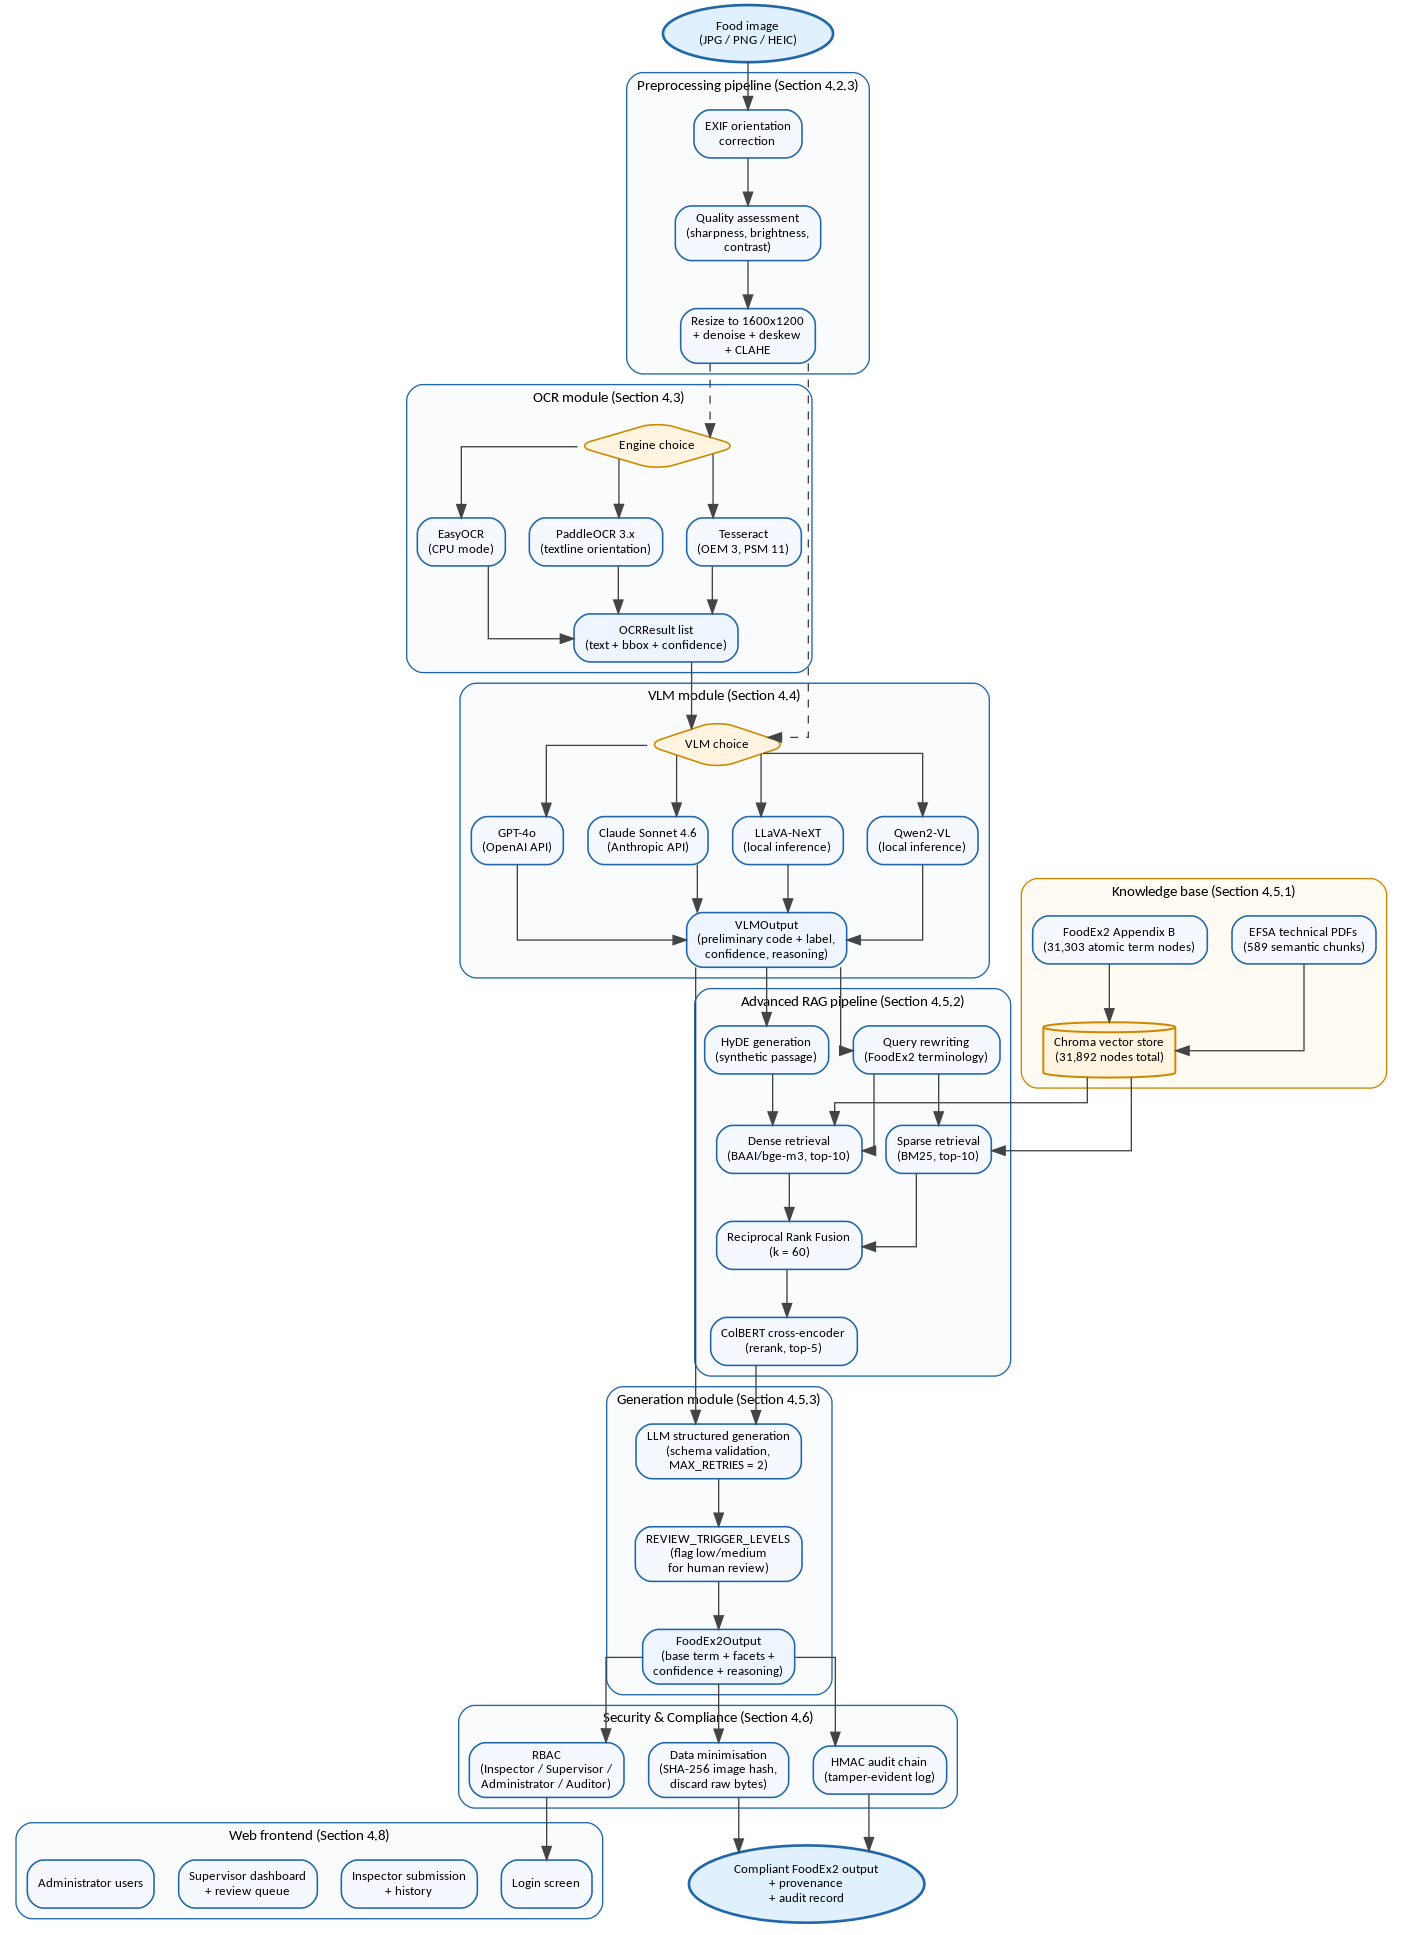
\includegraphics[width=0.85\linewidth,keepaspectratio]{fig1.png}
\caption{End-to-end architecture of the IDRISK2 pipeline. The diagram shows the flow from raw food image input through the preprocessing pipeline, OCR module (three engine options), VLM module (four model options), Advanced RAG pipeline with the FoodEx2 knowledge base, Generation module with structured FoodEx2 output, Security \& Compliance layer enforcing RBAC, data minimisation, and HMAC audit chaining, and the Web Frontend exposing role-specific views to inspectors, supervisors, administrators, and auditors.}
\end{figure}

\hypertarget{data-collection-and-preparation}{%
\section{Data Collection and Preparation}\label{data-collection-and-preparation}}

This section delineates the acquisition, annotation, and preprocessing protocols for the multimodal dataset employed in training and evaluating the IDRISK2 system, encompassing real-world photographs of both prepared dishes and packaged food products alongside the comprehensive FoodEx2 reference materials drawn from the EFSA Appendix B taxonomy.

\hypertarget{sources-of-food-product-data}{%
\subsection{Sources of Food Product Data}\label{sources-of-food-product-data}}

The evaluation dataset comprises real-world food images captured manually using smartphones under varied lighting and environmental conditions, intentionally introducing the visual challenges characteristic of real-world food safety inspections. The dataset deliberately mixes two complementary scenarios: photographs of prepared dishes served without packaging (the dominant case in restaurant or refectory inspections) and photographs of packaged commercial products with visible labels (the dominant case in retail inspections).

The dual-scenario composition reflects the architectural decision documented in Section 4.3.2 to treat OCR as a conditional rather than mandatory pipeline stage. Products span Portuguese, Brazilian, European, and international origins, with packaging labels in multiple languages including Portuguese, English, Spanish, French, and German, ensuring coverage of the multilingual variability expected in operational deployment. The preprocessing pipeline supports multiple input formats (JPG, PNG, WEBP, and HEIC, with HEIF/HEIC accepted via the pillow-heif dependency), and packaged products are photographed across multiple faces to capture the full label content.

The 34 images of the present evaluation set constitute a pilot study, intentionally curated to assess the system's performance in challenging, real-world conditions. Although this limited sample size restricts the statistical generalisation of the results, it provides a focused case study for demonstrating the architectural feasibility of the IDRISK2 pipeline. To ensure operational robustness, the system retains support for diverse image formats, despite the present evaluation set being captured and stored in JPG, accommodating the varied inputs typical of smartphone-based inspections. The empirical breakdown of this set is detailed in Section 5.3. Future efforts will address the scalability of this evaluation, aiming to incorporate larger datasets comparable to those used in established food classification research to further validate the system's robustness and regulatory applicability.

\hypertarget{data-annotation-for-foodex2}{%
\subsection{Data Annotation for FoodEx2}\label{data-annotation-for-foodex2}}

Each product sample is registered in the IDRISK2Dataset management system, which maintains a persistent index associating image paths with structured FoodEx2Annotation records. Each annotation captures the base term code and label, applicable facets with their descriptor codes, annotator identifier, annotation date, and a confidence level reflecting the annotator's certainty.

The annotation schema is designed to support multi-annotator validation: when more than one annotator processes the same image, the annotator\_id field distinguishes their independent judgements and inter-annotator agreement can be computed on the resulting paired annotations using Cohen's Kappa (two annotators) or Fleiss's Kappa (three or more). The empirical evaluation reported in Chapter 5 was carried out under single-annotator ground truth, a deliberate scope decision documented in Section 6.6, and the multi-annotator validation that the schema supports is reserved for the larger-scale evaluation described in Section 8.5.

\hypertarget{multimodal-data-preprocessing}{%
\subsection{Multimodal Data Preprocessing}\label{multimodal-data-preprocessing}}

The preprocessing pipeline, implemented in preprocessing.py, processes each image through four sequential stages. Images are first loaded with EXIF orientation correction to compensate for smartphone rotation metadata. A quality assessment stage then computes sharpness (Laplacian variance), brightness, and contrast metrics, flagging low-quality inputs for manual review. Accepted images undergo resizing to a standardised 1600\(\times\)1200 resolution with aspect-ratio-preserving padding, followed by denoising via fast non-local means filtering, deskewing via Hough line transform, and contrast enhancement via CLAHE in LAB colour space. Finally, a region-of-interest extraction stage uses adaptive thresholding and contour analysis to isolate text blocks, producing a binarised output optimised for OCR and an annotated image for visual inspection.

\hypertarget{ocr-and-image-processing-module}{%
\section{OCR and Image Processing Module}\label{ocr-and-image-processing-module}}

\hypertarget{ocr-engine-selection-and-fine-tuning}{%
\subsection{OCR Engine Selection and Fine-tuning}\label{ocr-engine-selection-and-fine-tuning}}

The selection of an OCR engine for the IDRISK2 pipeline is treated as an empirical decision informed by comparative evaluation across three candidate systems: Tesseract, EasyOCR, and PaddleOCR. All three engines are configured to support the four target languages present in the evaluation dataset, English, Portuguese, Spanish, and French, and evaluated on a held-out subset of preprocessed food label images under identical conditions. It is important to acknowledge that this comparative evaluation is constrained by the limited dataset size. Given the significant variability in fonts, curved surfaces, and lighting conditions inherent in food labels, this sample size may not fully ensure the robustness and generalisability of the selected engine. Future work should expand the test set to further validate these findings across more diverse operational conditions.

Tesseract is configured with the LSTM-based recognition engine (OEM 3) and sparse text page segmentation mode (PSM 11), which is appropriate for food labels where text is distributed non-linearly across the image rather than arranged in contiguous paragraphs. EasyOCR is initialised with the four target language models and run in CPU mode to ensure compatibility with the closed deployment environment. PaddleOCR is configured against its PaddleOCR 3.x API with textline orientation classification enabled (use\_textline\_orientation=True, the renamed successor of the angle-classification option from the 2.x API), which provides robustness to rotated text, a common characteristic of curved packaging surfaces captured by smartphone cameras. No specific PP-OCR model version is pinned in the deployment, so the default recognition model of the installed PaddleOCR release is used.

All three engines share a common output interface defined by the OCRResult dataclass, which standardises extracted text, bounding box coordinates in (x, y, width, height) format, and a per-token confidence score normalised to the range {[}0, 1{]}. This normalisation ensures that downstream components of the pipeline, including the VLM module and the RAG query construction, operate on a consistent representation regardless of the engine selected.

Engine performance is quantified using three complementary metrics: Character Error Rate (CER) and Word Error Rate (WER), computed against manually transcribed ground truth label text, and mean per-token confidence score. Processing time per image is additionally recorded to assess operational feasibility within the inspection workflow. The engine achieving the best aggregate performance across CER, WER, and processing time on the evaluation subset is selected as the default engine for the IDRISK2 pipeline, with the alternative engines retained as configurable options for deployment contexts with different label characteristics. Results of this comparative evaluation are reported in Section 5.3.

\hypertarget{computer-vision-for-product-identification}{%
\subsection{Computer Vision for Product Identification}\label{computer-vision-for-product-identification}}

Prior to OCR, each image passes through the preprocessing pipeline described in Section 4.2.3, producing a standardised 1600\(\times\)1200 image with corrected orientation, reduced noise, and enhanced contrast. The OCR module additionally applies adaptive thresholding to produce a binarised version of the preprocessed image, which is provided to Tesseract and used as a fallback input for EasyOCR and PaddleOCR when the colour image yields low-confidence results. Bounding boxes returned by each engine are post-processed to merge fragmented tokens belonging to the same word, using a horizontal proximity threshold calibrated to the target image resolution. The resulting structured output, a list of OCRResult objects with text, position, and confidence, is passed to the VLM module as part of the multimodal product representation.

\hypertarget{vision-language-model-selection-and-integration}{%
\section{Vision-Language Model Selection and Integration}\label{vision-language-model-selection-and-integration}}

\hypertarget{candidate-vlm-evaluation-gpt-4o-claude-llava}{%
\subsection{Candidate VLM Evaluation (GPT-4o, Claude, LLaVA)}\label{candidate-vlm-evaluation-gpt-4o-claude-llava}}

Three Vision-Language Models are implemented as interchangeable candidates for the central integration layer of the IDRISK2 pipeline: GPT-4o (OpenAI), Claude (Anthropic), and LLaVA (HuggingFace, open-source). The selection covers two principal deployment paradigms, proprietary cloud APIs and open-source local inference, and supports the architectural property of VLM substitutability documented in Section 4.4.3: switching from one VLM to another requires only changing a configuration entry and does not affect the retrieval or generation stages downstream.

GPT-4o is accessed via the OpenAI Chat Completions API and represents the proprietary cloud-based paradigm. It offers state-of-the-art multimodal reasoning capabilities and native support for high-resolution image inputs with configurable detail levels. Its reliance on an external API introduces latency variability and requires that the OpenAI processing agreement be acceptable under the deploying authority's data-governance policy; in operational deployments where this constraint cannot be satisfied, GPT-4o is substituted by one of the local alternatives below.

Claude is accessed via the Anthropic Messages API and represents an alternative proprietary cloud option with equivalent multimodal reasoning quality and a distinct safety-tuning regime. The motivating hypothesis for including Claude as a candidate is that the patterns of hallucination observed in structured-taxonomy classification (Section 6.4) may differ across proprietary models trained with different fine-tuning corpora and safety procedures, and a comparative evaluation across at least two strong proprietary VLMs is necessary to distinguish single-model failure modes from general failure modes of the VLM class. The default deployment uses claude-sonnet-4 for the balance of cost and quality, with claude-opus-4 available for highest-accuracy runs at increased cost and claude-haiku-4-5 for faster, cheaper inference where reasoning depth is less critical.

LLaVA is an open-source instruction-tuned VLM that combines a Vicuna or Mistral language backbone with a CLIP vision encoder, designed for local inference via the HuggingFace Transformers library. The default configuration uses LLaVA-NeXT (LLaVA-1.6) with the Mistral-7B backbone, which is the strongest open-source LLaVA variant at the time of writing. The open-source nature of the model makes it fully compatible with the closed deployment requirement of Section 4.6, and its instruction-following capabilities are well-suited to structured classification tasks with explicitly defined JSON output formats.

The empirical evaluation reported in Chapter 5 was conducted with all three implemented VLMs: GPT-4o (used as the primary configuration throughout Sections 5.3 to 5.6), Claude Sonnet 4.6 (used in the cross-VLM comparison of Section 5.7.2), and LLaVA-NeXT-Mistral-7B (used as the open-source baseline in the same comparison). The three implementations are retained in the production codebase to support deployment-time substitution of the VLM layer in operational contexts where the data-governance constraints of the proprietary APIs cannot be satisfied, or where a fully self-hosted configuration is required.

\hypertarget{prompt-engineering-for-foodex2-classification}{%
\subsection{Prompt Engineering for FoodEx2 Classification}\label{prompt-engineering-for-foodex2-classification}}

All three VLMs are governed by a unified structured prompting strategy designed to elicit precise, FoodEx2-compliant outputs in a consistent JSON format, despite the different prompt-template conventions of the underlying APIs. The prompt architecture consists of three components: a system prompt that defines the classification task, the FoodEx2 output schema, and the confidence rubric; a few-shot example drawn from the FoodEx2 documentation that illustrates the expected reasoning and output structure; and a per-sample user prompt that provides the OCR-extracted label text and instructs the model to analyse both the image and the text jointly before producing its classification. The three VLM-specific adapters in the implementation are responsible for translating this unified prompt into the API conventions of GPT-4o (Chat Completions messages with image\_url content blocks), Claude (Messages API with image content blocks under a top-level system field), and LLaVA-NeXT (Mistral chat template with an interleaved image token), without exposing those differences to downstream code.

Chain-of-thought reasoning is encouraged through the reasoning field of the required JSON output, which instructs the model to articulate its classification rationale step-by-step before committing to a final code assignment. This approach serves two purposes: it improves classification accuracy on ambiguous cases by forcing the model to reason explicitly through the evidence, and it produces a human-readable audit trail that supports the explainability requirements applicable to the system under the GDPR and the EU AI Act. Although this CoT-based transparency provides meaningful support for these obligations, it represents only one dimension of the broader, comprehensive legal compliance framework mandated for high-criticality AI systems.

Temperature is set to 0.1 across all models to minimise output variability and promote deterministic classification behaviour, consistent with the precision requirements of the FoodEx2 taxonomy. Prompt templates are refined iteratively on a development subset of the dataset, with systematic adjustments targeting the most frequent error categories identified in initial evaluations.

\hypertarget{multimodal-feature-integration}{%
\subsection{Multimodal Feature Integration}\label{multimodal-feature-integration}}

Each VLM receives as joint input the preprocessed food label image, encoded as a base64 JPEG string, and the OCR-extracted text produced by the module described in Section 4.3. This dual input design ensures that the model can leverage both the visual layout and spatial organisation of the label and the textual content extracted by the OCR engine, compensating for cases where one modality is unreliable, such as degraded OCR output on heavily stylised fonts, or partially occluded visual elements. The unified VLMOutput dataclass provides a model-agnostic representation of the classification result, including the base term code and label, applicable facets, reasoning chain, confidence level, and the raw model response retained for audit purposes.

\hypertarget{retrieval-augmented-generation-implementation}{%
\section{Retrieval-Augmented Generation Implementation}\label{retrieval-augmented-generation-implementation}}

\hypertarget{knowledge-base-construction-for-foodex2}{%
\subsection{Knowledge Base Construction for FoodEx2}\label{knowledge-base-construction-for-foodex2}}

The RAG knowledge base is constructed from two complementary sources published by the EFSA, each addressing a distinct retrieval need. The first source comprises the official FoodEx2 technical documentation: the original system description (The food classification and description system FoodEx2, Revision 2) together with the annual maintenance reports published between 2019 and 2025. These documents describe the taxonomy's governance, descriptor philosophy, facet semantics, and the year-on-year evolution of approved terms, context essential for interpreting why a given classification decision is correct, but insufficient on its own to surface candidate base term codes during retrieval.

The second source is the FoodEx2 Catalogue Browser export (Appendix B), distributed by EFSA as an XLSX workbook containing the full taxonomy: 31,303 approved terms and 298 deprecated terms organised across the hierarchy, reporting, exposure, ingredient, and pesticide views. Each row provides the term code, extended name, scope note, scientific and common names, and the implicit facet expression, the raw material that the generation component needs to assign a specific base term to a food product. Deprecated terms are filtered out at ingestion, as they are not valid targets for new classifications.

The two sources require different segmentation strategies. The technical PDFs are partitioned through LlamaIndex's SemanticSplitterNodeParser, which detects content boundaries using embedding-based similarity rather than fixed token counts, preserving descriptor definitions and classification rules as coherent semantic units. A fixed-size fallback strategy with 512-token chunks and 64-token overlap is retained as a configurable alternative for documents with less structured layouts. The taxonomy XLSX, by contrast, is ingested without further chunking: each FoodEx2 term is converted into a single atomic node whose chunk identifier mirrors the term code (for example, term\_A03VY). This decision reflects three considerations. First, each term entry is already a self-contained semantic unit of approximately 100--250 tokens, well within the embedding model's effective context window, so further splitting would gain nothing in retrieval precision. Second, partitioning a term across multiple chunks would scatter its name, scope note, and implicit facet expression into separate retrieval candidates, breaking the assumption that the cross-encoder reranker compares the query against complete term entries. Third, atomic term nodes establish a direct one-to-one mapping between citations and FoodEx2 codes, ensuring that every chunk identifier in an audit record can be deterministically resolved to a single taxonomy entry, a property essential for the explainability and post-hoc inspection requirements of Article 22 of the GDPR.

Both source streams are encoded into dense vector representations using the BAAI/bge-m3 multilingual embedding model, selected for its strong performance on technical domain text and its native support for the four target languages of the evaluation dataset. The model runs entirely locally, without external API dependency, ensuring GDPR compliance throughout the indexing pipeline. The combined corpus, approximately 31,900 nodes in the final configuration, is stored in a Chroma persistent vector store, enabling efficient approximate nearest neighbour search at inference time.

Knowledge base provenance is recorded in a manifest file capturing the full set of source files (PDFs and XLSX), the FoodEx2 version identifier (FoodEx2-Appendix-B for taxonomy nodes, with PDF-side version detection retained for the technical documents), the embedding model, the chunking strategy applied to each stream, the total node count, and a SHA-256 checksum computed over all node texts. This checksum enables cryptographic integrity verification at deployment time, detecting any unauthorised modification of the retrieval index that could propagate errors into the classification pipeline. The full heterogeneous-chunking knowledge-base construction methodology is illustrated in Figure 4.2.

\begin{figure}[htbp]
\centering
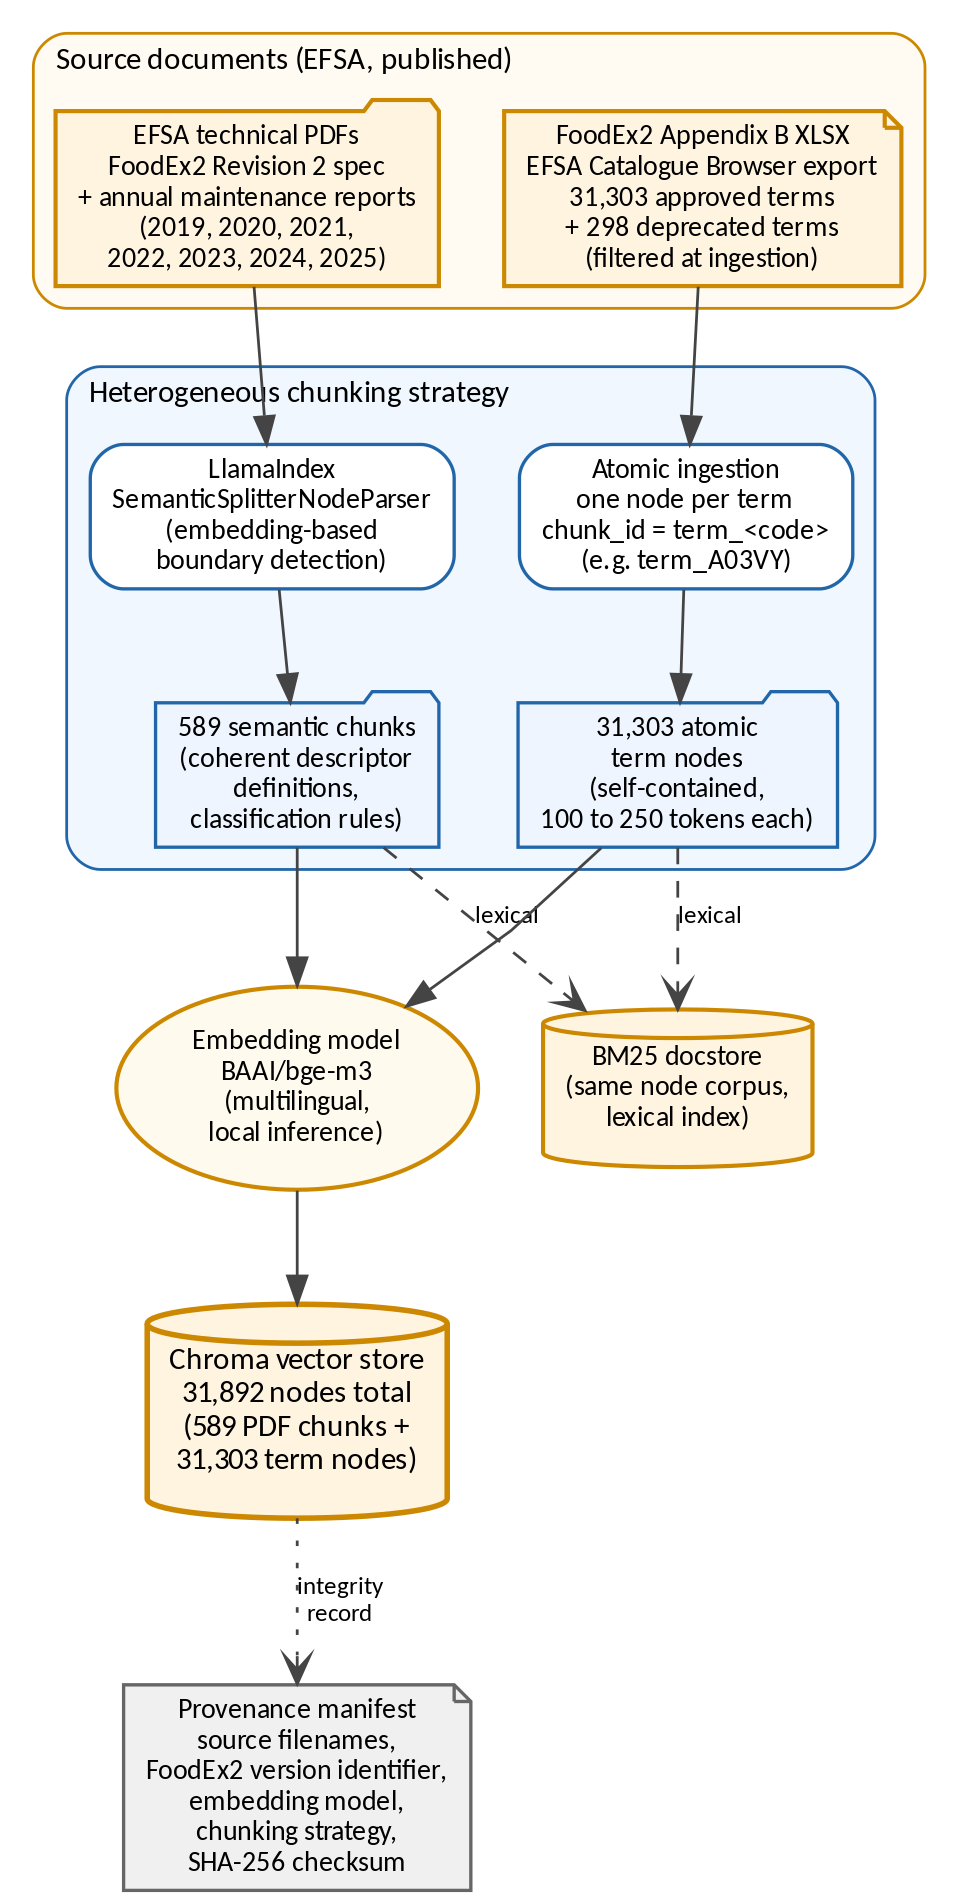
\includegraphics[width=0.85\linewidth,keepaspectratio]{fig2.png}
\caption{Heterogeneous knowledge-base construction methodology (Section 4.5.1). Two source streams published by EFSA, the FoodEx2 technical PDFs (Revision 2 and the 2019 to 2025 annual maintenance reports) and the Appendix B XLSX catalogue (31,303 approved terms after filtering 298 deprecated entries), are ingested through distinct chunking strategies tailored to their respective structure: semantic splitting via LlamaIndex's SemanticSplitterNodeParser for the PDFs (589 chunks preserving descriptor definitions and classification rules as coherent semantic units) and atomic ingestion for the XLSX (one node per term with chunk\_id mirroring the term code). Both streams are encoded with the BAAI/bge-m3 multilingual embedding model under fully local inference and stored in the Chroma persistent vector store (31,892 nodes total), with a parallel BM25 docstore over the same corpus supporting lexical retrieval. A provenance manifest records source filenames, FoodEx2 version identifier, embedding model, chunking strategy, and a SHA-256 checksum over all node texts for cryptographic integrity verification at deployment time.}
\end{figure}

\hypertarget{advanced-rag-pipeline-design}{%
\subsection{Advanced RAG Pipeline Design}\label{advanced-rag-pipeline-design}}

The retrieval component implements an Advanced RAG architecture organised into three sequential stages: pre-retrieval enhancement, hybrid retrieval, and post-retrieval refinement. The end-to-end data flow is illustrated in Figure 4.3.

At the pre-retrieval stage, the multimodal product description produced by the VLM module undergoes two parallel transformations. Query rewriting reformulates the description using FoodEx2 terminology, compensating for vocabulary mismatches between colloquial product language and the technical vocabulary of the EFSA documentation. Hypothetical Document Embedding (HyDE) generates a synthetic passage mimicking the style and terminology of the FoodEx2 technical guidelines, which is used as the primary retrieval query for dense search, replacing the original description with a representation that is semantically closer to the indexed content and therefore more likely to surface the most relevant taxonomy entries.

The retrieval stage combines dense semantic search over the Chroma vector store with sparse BM25 lexical retrieval. Dense retrieval returns the top-10 candidates ranked by cosine similarity to the HyDE-generated query embedding, capturing semantically related passages even when exact terminology differs. Sparse retrieval applies BM25 to the rewritten query, returning the top-10 candidates ranked by term frequency statistics, ensuring that passages containing specific FoodEx2 base term codes or facet descriptors are surfaced even if their semantic embedding is not among the closest neighbours. The two candidate sets are merged using Reciprocal Rank Fusion with the standard constant k = 60, which assigns a combined score to each unique passage based on its rank position in both retrieval lists, producing a single unified ranking that leverages the complementary strengths of both approaches.

At the post-retrieval stage, the fused candidate set is reranked using a ColBERT cross-encoder, which performs token-level interaction between the rewritten query and each passage to produce more precise relevance scores than the bi-encoder similarity used in dense retrieval. The reranked passages are subsequently filtered by a minimum similarity threshold, deduplicated to remove near-identical content, and truncated to a maximum context length of 6,000 characters to ensure compatibility with the generation component's context window. Each retained passage is tagged with its source document filename and chunk identifier, providing a traceable reference for every element of the context injected into the generation prompt.

\begin{figure}[htbp]
\centering
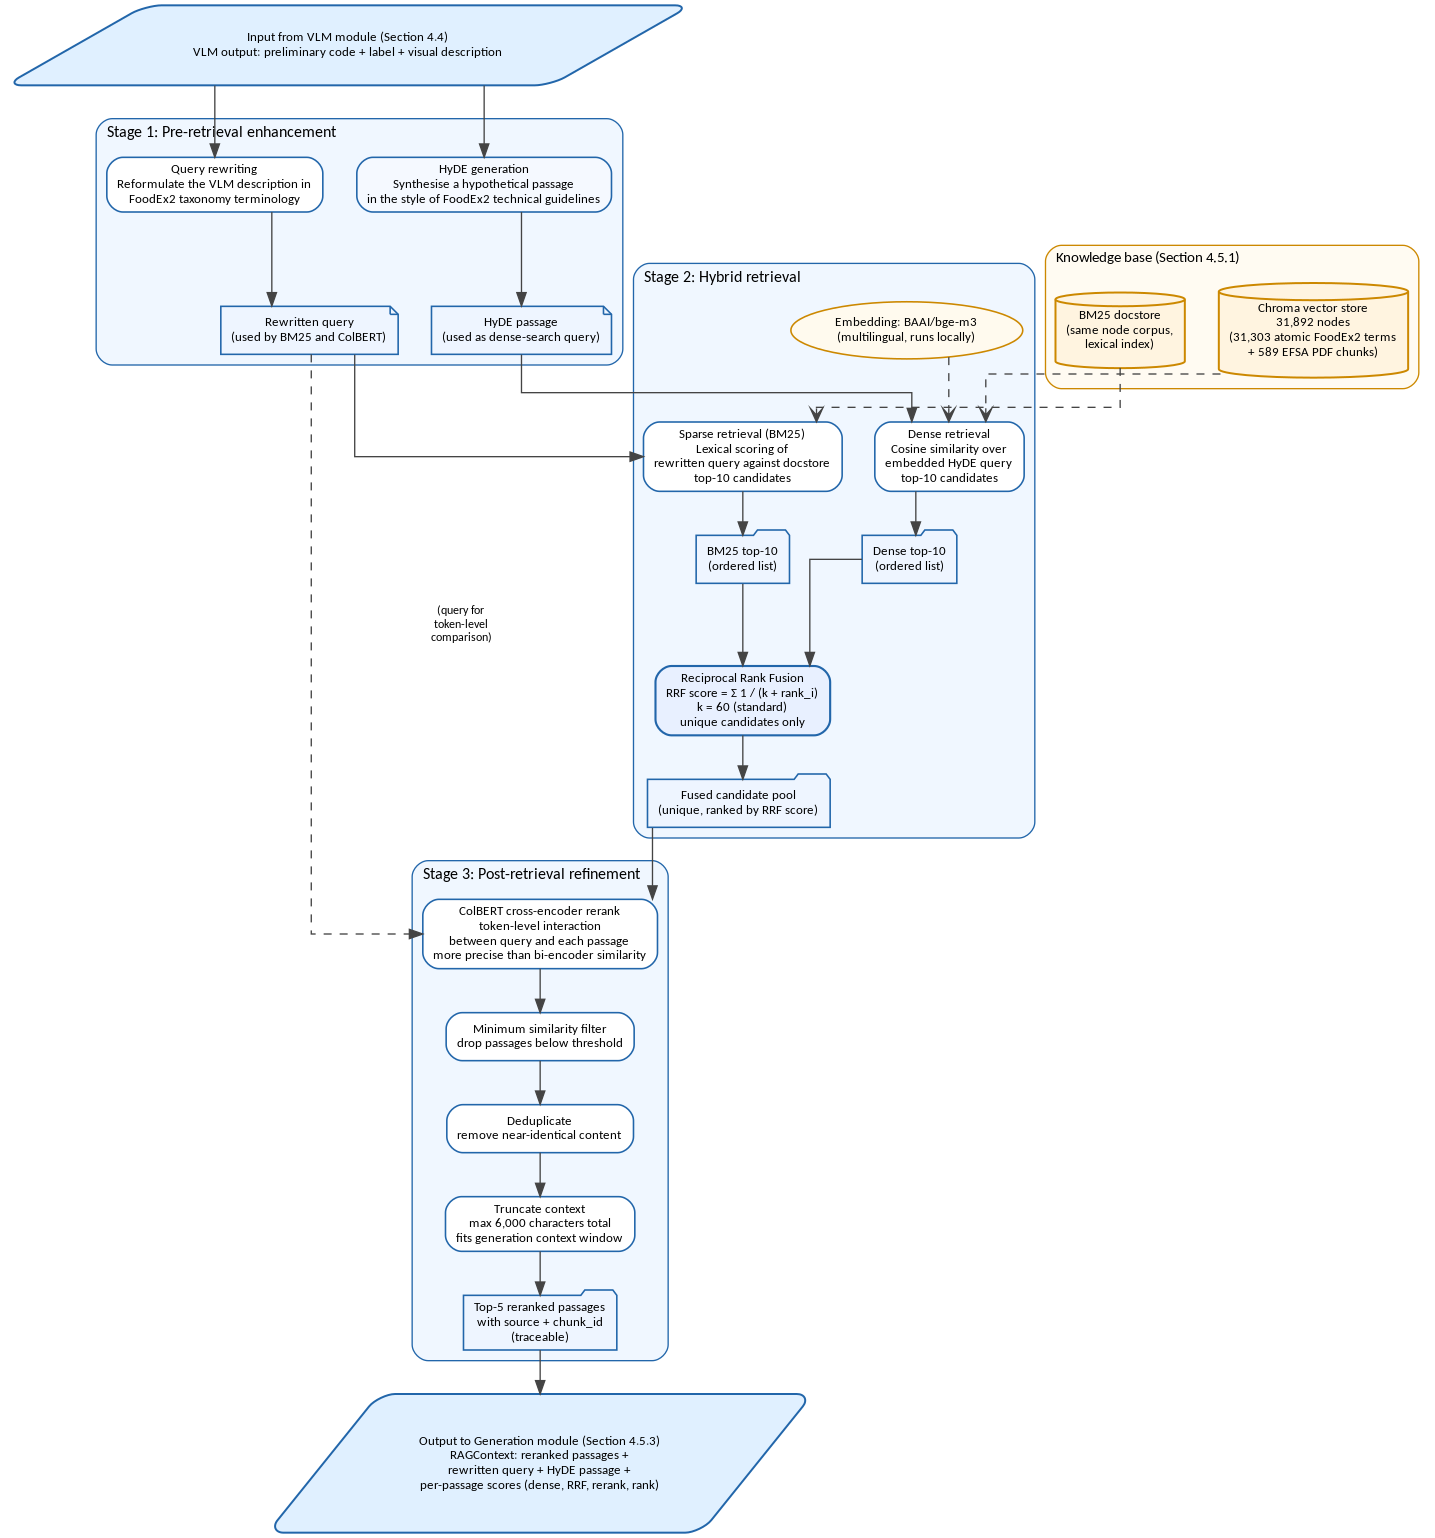
\includegraphics[width=0.85\linewidth,keepaspectratio]{fig3.png}
\caption{Detailed architecture of the Advanced RAG pipeline (Section 4.5.2). Stage 1 performs query rewriting and HyDE synthesis on the VLM-produced multimodal description. Stage 2 executes hybrid retrieval: dense semantic search using the BAAI/bge-m3 embedding over the HyDE passage and BM25 lexical retrieval over the rewritten query, both returning the top-10 candidates from the Chroma-backed corpus, with the two ranked lists merged through Reciprocal Rank Fusion (k = 60). Stage 3 reranks the fused pool with a ColBERT cross-encoder, filters passages below a similarity threshold, deduplicates near-identical content, and truncates the context to 6,000 characters before passing the top-5 traceable passages, together with their dense, RRF, and rerank scores, to the Generation module described in Section 4.5.3.}
\end{figure}

\hypertarget{generation-component-for-foodex2-classification}{%
\subsection{Generation Component for FoodEx2 Classification}\label{generation-component-for-foodex2-classification}}

The generation component receives the compressed, reranked retrieval context assembled by the pipeline described in Section 4.5.2 and produces a structured FoodEx2 classification output grounded exclusively in the retrieved EFSA documentation. The generation prompt is structured in two parts: a system prompt that defines the classification task, the required JSON output schema, and the instruction to base all classification decisions solely on the provided context; and a user prompt that presents the retrieved passages alongside the multimodal product description produced by the VLM module.

The system prompt explicitly instructs the model to cite specific retrieved passages in its reasoning, establishing a direct traceable link between each element of the classification output and the corresponding FoodEx2 documentation. This design ensures that the system's decisions are not only grounded in authoritative regulatory content but are also explainable and auditable, satisfying the transparency requirements of Article 22 of the GDPR and the documentation obligations of the EU AI Act for high-risk AI systems.

Output validation enforces the required FoodEx2 schema, comprising the base term code, base term label, facets dictionary, reasoning chain, and confidence level, through a structured parsing and validation function. If the initial generation fails schema validation, the system automatically retries up to two times with a corrective prompt, before defaulting to an UNKNOWN classification with low confidence flagged for human review. The human-review policy is governed by a configurable REVIEW\_TRIGGER\_LEVELS set, which by default flags any classification with low or medium confidence, leaving only high-confidence outputs to proceed without oversight. This conservative default aligns with the human-oversight requirement of Article 14 of the EU AI Act for high-risk AI systems, and can be relaxed by supplying a custom trigger set (e.g. \{Confidence.LOW\}) to the generation component for deployment contexts that tolerate greater autonomy.

Each classification decision is persisted as a structured JSON audit record containing the full classification result, the retrieved source documents and chunk identifiers, the model used, the timestamp, the raw generation output, and the human review flag. This audit trail supports post-hoc inspection of any classification decision and provides the documentation required for regulatory accountability.

\hypertarget{security-and-privacy-enhancements}{%
\section{Security and Privacy Enhancements}\label{security-and-privacy-enhancements}}

\hypertarget{secure-model-deployment}{%
\subsection{Secure Model Deployment}\label{secure-model-deployment}}

The IDRISK2 system is designed for fully self-hosted deployment, with all model inference, including OCR, VLM processing, and RAG generation, performed locally on infrastructure controlled by the deploying organisation. No product data is transmitted to external services at any stage of the pipeline, ensuring compatibility with the data governance requirements of official regulatory bodies and the principle of privacy by design mandated by Article 25 of the GDPR.

Access to the system is governed by a role-based access control framework defining four roles: Inspector, Supervisor, Administrator, and Auditor. Each role is assigned a specific set of permissions, including submission of classification requests, access to results, management of the knowledge base, and access to audit records, enforced at the function level through a permission decorator that logs and rejects unauthorised access attempts. This granular access model ensures that sensitive system functions are accessible only to authorised personnel, in accordance with the principle of least privilege.

Input validation is applied to all incoming data before processing. Image inputs are validated against maximum size constraints, an allowed MIME type allowlist, and magic byte verification to detect format spoofing. OCR-extracted text is sanitised to remove control characters and truncated to a maximum length prior to prompt injection, mitigating the risk of prompt injection attacks through maliciously crafted label content.

\hypertarget{gdpr-compliance-mechanisms}{%
\subsection{GDPR Compliance Mechanisms}\label{gdpr-compliance-mechanisms}}

Data minimisation is enforced at the record level through the MinimisedProductRecord dataclass, which retains only the OCR-extracted text, the FoodEx2 classification result, and a SHA-256 hash of the original image for deduplication purposes. Raw image bytes are discarded immediately after feature extraction, in accordance with Article 5(1)(c) of the GDPR. Each minimised record is subsequently persisted as a JSON document in the configured records directory by the save\_minimised\_record function, enabling subsequent retrieval for legitimate purposes while preserving the deletion of raw image content. A configurable retention policy automatically deletes classification records after one year and audit logs after seven years, reflecting standard regulatory retention requirements.

Audit logging is implemented through a tamper-evident HMAC chaining mechanism. Each audit entry records the event type, user identifier, event details, timestamp, and an HMAC computed over the entry content keyed to a deployment-specific secret. Each entry additionally includes the HMAC of the preceding entry, forming a cryptographically linked chain that renders any post-hoc modification detectable through the verify\_chain method. To preserve the integrity of this verification, audit storage is partitioned into two distinct directories: a chain-verified directory holding only the tamper-evident HMAC entries written by the AuditLogger, and a separate generation-records directory holding the per-classification provenance records emitted by the generation component. This separation prevents the unstructured generation records from being misinterpreted as broken links during chain verification. Together, the two directories satisfy the documentation and traceability obligations of the EU AI Act for high-risk AI systems, enabling post-hoc inspection of any classification decision by authorised auditors.

System configuration is managed exclusively through environment variables, with required variables validated at startup. Sensitive credentials, including the audit HMAC key and, where applicable, the OpenAI API key (for GPT-4o) or the Anthropic API key (for Claude), are never hardcoded or persisted in source files, in accordance with secure credential management best practices.

\hypertarget{implementation-notes}{%
\section{Implementation Notes}\label{implementation-notes}}

\hypertarget{technology-stack}{%
\subsubsection{Technology Stack}\label{technology-stack}}

The IDRISK2 system is implemented in Python 3.11, selected for its mature ecosystem of AI and computer vision libraries and its widespread adoption in academic research contexts. Table 4.1 summarises the principal technologies and frameworks used across the pipeline modules.

\begin{longtable}[]{@{}lll@{}}
\caption{Technology stack of the IDRISK2 system}\label{tab:tech-stack}\\
\toprule
\endhead
\textbf{Component} & \textbf{Technology} & \textbf{Version}\tabularnewline
RAG Framework & LlamaIndex & \(\ge\) 0.10.40\tabularnewline
Vector Store & ChromaDB & \(\ge\) 0.5.0\tabularnewline
Embedding Model & BAAI/bge-m3 &\tabularnewline
Sparse Retriever (BM25) & llama-index-retrievers-bm25 & \(\ge\) 0.2.0\tabularnewline
Cross-encoder Reranker (ColBERT) & llama-index-postprocessor-colbert-rerank & \(\ge\) 0.1.4\tabularnewline
FoodEx2 XLSX ingestion & openpyxl & \(\ge\) 3.1.2\tabularnewline
OCR, Option A & Tesseract / pytesseract & \(\ge\) 0.3.13\tabularnewline
OCR, Option B & EasyOCR & \(\ge\) 1.7.1\tabularnewline
OCR, Option C & PaddleOCR & \(\ge\) 2.7.3\tabularnewline
VLM, Option A & GPT-4o (OpenAI API) & openai \(\ge\) 1.30.0\tabularnewline
VLM, Option B & Claude (Anthropic API) & anthropic \(\ge\) 0.34.0\tabularnewline
VLM, Option C & LLaVA-NeXT (HuggingFace) & transformers \(\ge\) 4.45.0\tabularnewline
Image Processing & OpenCV & \(\ge\) 4.9.0\tabularnewline
HEIC Support & pillow-heif & \(\ge\) 0.16.0\tabularnewline
LLM Generation & OpenAI SDK & \(\ge\) 1.30.0\tabularnewline
Evaluation Metrics (CER/WER) & editdistance & \(\ge\) 0.8.1\tabularnewline
Frontend Framework & React + TypeScript + Vite & React \(\ge\) 18\tabularnewline
UI Component Library & shadcn/ui (Radix UI primitives) &\tabularnewline
Styling & Tailwind CSS & \(\ge\) 4.0\tabularnewline
Data Visualisation (frontend) & Recharts &\tabularnewline
\bottomrule
\end{longtable}


\hypertarget{project-structure}{%
\subsubsection{Project Structure}\label{project-structure}}

The codebase is organised into two top-level deliverables: the Python backend that implements the classification pipeline described in Sections 4.2--4.6, and the web frontend that exposes the pipeline through role-based screens as documented in Section 4.8.

\begin{verbatim}
Dissertação/
|-- idrisk2/ <- Python backend (classification pipeline)
| |-- pipeline.py <- End-to-end pipeline entry point
| |-- requirements.txt <- Dependency specification
| `-- src/
| |-- common/types.py <- Shared Confidence enum and review-trigger policy
| |-- data/preprocessing.py <- Image loading and preprocessing (4.2)
| |-- ocr/engine.py <- OCR engine abstraction and benchmarking (4.3)
| |-- vlm/vlm.py <- VLM integration: GPT-4o, Claude, LLaVA-NeXT (4.4)
| |-- rag/
| | |-- knowledge_base.py <- FoodEx2 knowledge base construction (4.5.1)
| | |-- retrieval.py <- Advanced RAG retrieval pipeline (4.5.2)
| | `-- generation.py <- FoodEx2 generation and audit (4.5.3)
| `-- security/security.py <- RBAC, audit logging, GDPR mechanisms (4.6)
|
`-- Idrisk2webappinterface/ <- Web frontend (inspector workflow UI)
|-- src/
| |-- App.tsx <- Role-based routing (Inspector/Supervisor/Admin/Auditor)
| |-- components/
| | |-- LoginScreen.tsx <- Role-aware authentication
| | |-- InspectorSubmission.tsx <- Image upload + live pipeline progress
| | |-- InspectorHistory.tsx <- Per-user classification history
| | |-- SupervisorDashboard.tsx <- Metrics, review queue, confidence charts
| | `-- AdministratorUsers.tsx <- User and role management
| `-- components/ui/ <- shadcn/ui primitives (Radix UI)
|-- package.json
`-- vite.config.ts <- Vite build configuration
\end{verbatim}

\hypertarget{installation-and-configuration}{%
\subsubsection{Installation and Configuration}\label{installation-and-configuration}}

The system is configured entirely through environment variables, consistent with the secure configuration management approach described in Section 4.6.2. Prior to execution, the following variables must be set:

\begin{verbatim}
# Required
export IDRISK2_AUDIT_KEY="<secure-random-key>"
export IDRISK2_DATA_DIR="/path/to/data"
export IDRISK2_DOCS_DIR="/path/to/efsa/documents"
# Required only if using the GPT-4o VLM (default)
export OPENAI_API_KEY="<openai-api-key>"
# Required only if using the Claude VLM
export ANTHROPIC_API_KEY="<anthropic-api-key>"
# Optional VLM selection: gpt4o (default) | claude | llava
export IDRISK2_VLM_MODEL="gpt4o"
\end{verbatim}

Backend dependencies are installed via:

\begin{quote}
cd idrisk2

pip install -r requirements.txt
\end{quote}

The web frontend described in Section 4.8 is installed and started separately:

\begin{verbatim}
cd Idrisk2webappinterface
pnpm install
pnpm dev # development server (Vite)
pnpm build # production build
\end{verbatim}

A classification request can be submitted programmatically against the backend as follows:

\begin{quote}
from pipeline import IDRISK2Pipeline

from src.security.security import User, Role

pipeline = IDRISK2Pipeline.from\_env()

user = User(

user\_id="u001",

username="inspector\_a",

role=Role.INSPECTOR,

created\_at="2025-01-01",

)

result = pipeline.classify(

image\_path="product\_label.jpg",

user=user,

)

print(result.classification.base\_term\_code)

print(result.classification.reasoning)
\end{quote}

In normal operational use, the same call is invoked through the web frontend's Inspector Submission screen, with the User object resolved at login time from the authenticated role (Section 4.8).

\hypertarget{web-interface-for-operational-deployment}{%
\section{Web Interface for Operational Deployment}\label{web-interface-for-operational-deployment}}

The IDRISK2 pipeline as documented in Sections 4.2--4.6 exposes a programmatic API; for the inspector and supervisor workflows that motivate the system in Section 1.2, a graphical user interface is required to make the pipeline operationally usable in the field. This section describes the web frontend that exposes the pipeline through role-aware screens aligned with the role-based access control framework defined in Section 4.6.1.

The frontend is implemented as a single-page application using React 18 with TypeScript, built and bundled with Vite. Component primitives are drawn from the shadcn/ui library, which is itself layered over Radix UI, and styled with Tailwind CSS v4 to ensure consistent visual presentation across the role-specific views. Data visualisations on the supervisor dashboard are rendered with Recharts, chosen for its compatibility with the React component model and its declarative API for the time-series and distribution plots required by the review-queue and confidence-distribution views. The full frontend technology stack is reported in Table 4.1 alongside the backend dependencies, and the project layout is shown in the codebase tree above.

The application's routing layer enforces the role-based access control framework of Section 4.6.1: the four roles defined in that framework (Inspector, Supervisor, Administrator, and Auditor) are surfaced as distinct top-level views, with the available navigation determined at login time by the role attached to the authenticated user. The roles defined in the backend permissions table thus map directly to the menu structure of the frontend, ensuring that no screen exposes functionality beyond what the backend's permission decorator would authorise, defence-in-depth between the presentation layer and the API layer, rather than client-side gating alone.

Five screens implement the operational workflows of the system. The login screen accepts credentials and resolves the user's role, redirecting to the appropriate landing view. The Inspector submission screen accepts image uploads and renders a progress bar that tracks the pipeline through its sequential stages, OCR, VLM, RAG retrieval, and final classification, providing live visibility into the per-image latency profile reported in Section 5.6. The Inspector history screen presents the inspector's own past classifications with their final FoodEx2 codes, confidence levels, and audit identifiers, drawn from the minimised product records persisted by the save\_minimised\_record function of Section 4.6.2. The Supervisor dashboard aggregates the team-level view: review-queue items flagged by the human-review trigger of Section 4.5.3, distribution plots over confidence levels, and per-day classification throughput. The Administrator user-management screen exposes the create-update-deactivate operations for users and role assignments, subject to the manage\_users permission defined in Section 4.6.1.

This frontend is the user-facing component of the decision-support deployment model proposed in Section 6.4. The progress visualisation surfaces the system's latency profile to the inspector at submission time, the supervisor dashboard's review queue materialises the human-oversight mechanism that the EU AI Act requires for high-risk AI systems, and the per-classification provenance records described in Section 4.6.2 are made directly visible to supervisors and auditors through the history and dashboard screens. Full operational deployment in a regulatory authority would require the additional integration work with LIMS, inspection-workflow systems, and the EFSA Data Collection Framework outlined in Section 8.3; the present implementation establishes the user-facing layer required for any such deployment and is ready to operate as a standalone decision-support tool in supervised pilot contexts.
  % Methodology
\hypertarget{evaluation-and-results}{%
\chapter{Evaluation and Results}\label{evaluation-and-results}}

This chapter reports the empirical evaluation of the IDRISK2 system on a dataset of 34 real-world food images. The evaluation focuses on three dimensions: the per-layer performance of each pipeline component (OCR, VLM, RAG retrieval), the end-to-end classification accuracy against a manually annotated FoodEx2 ground truth, and the calibration of the system's confidence and human-review mechanisms with respect to actual classification correctness. The metrics presented in this chapter form the empirical basis for the discussion of the system's strengths and limitations developed in Chapter 6.

\hypertarget{evaluation-metrics}{%
\section{Evaluation Metrics}\label{evaluation-metrics}}

\hypertarget{foodex2-classification-accuracy}{%
\subsection{FoodEx2 Classification Accuracy}\label{foodex2-classification-accuracy}}

Two complementary accuracy metrics are defined to capture the strict and lenient interpretations of correct classification within the FoodEx2 taxonomy. Exact-match accuracy is the proportion of system outputs whose base term code is identical to the ground truth code; this is the strictest interpretation, treating any divergence from the annotated code as incorrect. Family-level accuracy is the proportion of outputs whose code shares the same first three characters as the ground truth code, which corresponds to membership in the same FoodEx2 hierarchy branch (for example A03Z* for sandwich-class terms, A040* for cooked pasta-based dishes); this complementary metric captures cases where the system is in the correct semantic neighbourhood but missed the specific sub-type.

\hypertarget{ocr-accuracy}{%
\subsection{OCR Accuracy}\label{ocr-accuracy}}

OCR-extracted text is reported in terms of token count per image and the rate of non-empty OCR output across the evaluation set. Because the dataset is dominated by photographs of prepared dishes without packaging text, the relevant question is not OCR character error rate but the proportion of images for which the OCR layer contributes any usable signal to the downstream pipeline. Where OCR did extract content, the sanitised token strings are reported alongside the corresponding final classification for traceability.

\hypertarget{rag-retrieval-quality}{%
\subsection{RAG Retrieval Quality}\label{rag-retrieval-quality}}

The quality of the RAG retrieval layer is evaluated through three complementary measures. The mean rerank score of the top-1 retrieved candidate measures the cross-encoder's confidence in the most relevant passage. The proportion of retrieved passages that are FoodEx2 taxonomy terms (atomic nodes, prefixed term\_) versus EFSA documentation chunks (prefixed chunk\_) measures whether the retriever is surfacing the appropriate type of content for classification grounding. The RAG uplift rate measures the proportion of cases where the post-retrieval final classification differs from, and is closer to ground truth than, the VLM's preliminary code, quantifying the RAG layer's contribution to system accuracy.

\hypertarget{calibration-metrics}{%
\subsection{Calibration Metrics}\label{calibration-metrics}}

Calibration is the alignment between the system's expressed confidence and the actual correctness of its outputs. The false high-confidence rate is the proportion of high-confidence outputs that are incorrect. The silent error rate is the proportion of incorrect outputs that escape the human-review trigger. Together, these two metrics measure whether the system's calibration honours the EU AI Act Article 14 requirement for meaningful human oversight in high-risk AI applications.

\hypertarget{system-throughput-and-latency}{%
\subsection{System Throughput and Latency}\label{system-throughput-and-latency}}

Latency is measured per image as the wall-clock time between the submission of an image to the pipeline and the emission of the final FoodEx2 classification, including OCR, VLM inference, RAG retrieval, reranking, and structured generation. Throughput is reported as the inverse of the mean per-image latency aggregated across the evaluation set, to provide an estimate of operational feasibility in inspection workflow contexts.

\hypertarget{experimental-setup}{%
\section{Experimental Setup}\label{experimental-setup}}

\hypertarget{dataset-description}{%
\subsection{Dataset Description}\label{dataset-description}}

The evaluation dataset comprises 34 photographs of food products and prepared dishes spanning Portuguese, Brazilian, and other international cuisines. The selection deliberately oversamples culturally specific dishes (feijoada, brigadeiro, francesinha, pastel de nata, acarajé) and Brazilian or Portuguese branded products (Sumol, Guaraná Antarctica, Ucal) to expose the system to inputs that lie outside the European-dominated coverage of the FoodEx2 taxonomy. Three of the 34 images are independent photographs of the same dish (francesinha.jpg, francesinha2.jpg, francesinha3.jpg), included to measure the system's stability across visual variations of an identical underlying food item. Images vary in resolution from 474\(\times\)474 to 2048\(\times\)1154 pixels and were captured under heterogeneous lighting conditions characteristic of real-world inspection scenarios.

For each image, a ground truth FoodEx2 base term code was assigned manually through an interactive annotation tool that presented the human annotator with the five candidates surfaced by the RAG retriever, the system's final classification, and a keyword search interface against the full 31,303-term taxonomy. Annotation decisions were made by inspecting the image and applying the FoodEx2 classification methodology: selecting the most specific applicable base term, falling back to a hierarchical parent term when no specific term applies, and adopting the base-term-plus-facet approach for compositions that exceed any single available code. The complete ground truth annotation set is recorded in data/ground\_truth.json and forms the reference against which all accuracy metrics in this chapter are computed.

\hypertarget{baseline-models}{%
\subsection{Baseline Models}\label{baseline-models}}

The system's RAG-augmented classification is compared against two baselines. The first is the bare VLM output: the preliminary FoodEx2 code emitted by the Vision-Language Model in its first inference pass, before any retrieval grounding. This baseline isolates the contribution of the RAG layer to overall accuracy. The second is the system's family-level classification, which credits the system for assignments that fall within the correct FoodEx2 hierarchy branch even when the specific code differs from the ground truth; this baseline allows the discussion to separate errors of granularity from errors of semantic misclassification.

\hypertarget{results-of-ocr-and-image-processing}{%
\section{Results of OCR and Image Processing}\label{results-of-ocr-and-image-processing}}

The OCR layer extracted at least one token from 8 of the 34 evaluation images, corresponding to a non-empty-output rate of 23.5\%. The eight images for which OCR contributed signal were all photographs of packaged commercial products with visible labels: croissaint (4 tokens), guarana (9 tokens), hamburguer (2 tokens), salgadinho (9 tokens), sumol (9 tokens), tosta\_com\_humus (21 tokens), tosta\_mista (2 tokens), and ucal (13 tokens). The remaining 26 images, all of which depict prepared dishes served without packaging, yielded zero OCR tokens.

This result confirms the methodological decision documented in Section 4.3.2 to treat OCR as a conditional rather than mandatory pipeline stage: in a substantial majority of operational classification requests, particularly those involving cooked dishes photographed at the point of consumption or inspection, no useful textual content exists on the image to be recognised. The system's tolerance for empty OCR output is therefore a structural requirement, not an edge case. Where OCR did extract content, the recovered tokens were typically degraded, for example, the Sumol can produced the string "Voriginal ) erasil {[}Quonaná AnTA RCTica 3SOml Uneunele unieiieotanzame 'Gulaani'", reflecting the visual complexity (curved surfaces, glare, stylised typography) of commercial food packaging. Despite the imperfect transcription, the OCR-derived tokens contributed measurable signal to the VLM's subsequent visual classification in all eight packaged-product cases, with the VLM correctly identifying the brand and product type from a combination of visual cues and degraded OCR fragments.

\hypertarget{results-of-llm-based-information-extraction}{%
\section{Results of LLM-based Information Extraction}\label{results-of-llm-based-information-extraction}}

The Vision-Language Model (GPT-4o) was evaluated as the source of the initial FoodEx2 code assignment, prior to any RAG grounding. Three distinct findings emerge from this evaluation, each material to the discussion of hallucination mitigation in Chapter 6.

First, the exact-match accuracy of the VLM's preliminary codes against the ground truth is zero out of 34, or 0.0\%. No image in the evaluation set received a correct base-term assignment from the VLM alone.

Second, a verification of the VLM-emitted codes against the FoodEx2 Appendix B taxonomy revealed that 94\% (32/34) of the VLM codes are real taxonomy entries that describe entirely unrelated concepts, while the remaining 6\% (2/34) are codes that do not exist in the taxonomy at all. The codes generated by the VLM consistently followed the structural format of FoodEx2 base terms (the letter A followed by four alphanumeric characters) but the mapping between code and food was systematically fabricated. Representative examples include the code A0FQJ, which the VLM repeatedly assigned to mixed meat-and-vegetable dishes with the claimed label "Mixed dish with meat and vegetables" but which corresponds in the official taxonomy to "Pigeye shark (as animal)"; A0EKC, assigned to fried plantains and sandwiches alike, which is officially "Live vegetables for infusions (as part-nature)"; and A0C9N, used for sushi and tosta mista, which is officially "Young bulls (1-2 years) for dairy". A small number of codes recur as VLM fallbacks, reused across heterogeneous inputs: A0FQJ appeared five times, A0EKC four times, and A0EJX three times, a pattern consistent with parametric memorisation of plausible-looking but semantically arbitrary FoodEx2 identifiers.

Third, the VLM expressed high confidence in 33 of its 34 preliminary classifications and medium confidence in only 1 (francesinha3.jpg). The confidence signal therefore provides no useful information about the actual probability of correctness, a phenomenon that propagates into the downstream classifier and undermines the human-review trigger discussed in Section 5.6.

These findings establish that, when evaluated in isolation, the VLM operates as a confidently hallucinatory taxonomy assigner. The format of its outputs is well-formed and the natural-language descriptions of the images are accurate; the failure mode is specifically the binding of FoodEx2 identifiers to images, which the parametric model does not have reliable knowledge to perform. The classification system as a whole would therefore be entirely unusable in the absence of the retrieval-grounded correction implemented by the RAG layer.

\hypertarget{results-of-retrieval-augmented-generation}{%
\section{Results of Retrieval-Augmented Generation}\label{results-of-retrieval-augmented-generation}}

The RAG retrieval layer surfaced five reranked passages per classification, drawn from a Chroma-backed index of 31,892 nodes (589 chunks from EFSA technical PDFs plus 31,303 atomic taxonomy term nodes). The mean rerank score of the top-1 candidate across the 34 images is 0.693 (median 0.700, minimum 0.581, maximum 0.761). For every image in the evaluation set, all five retrieved passages were taxonomy terms, no PDF chunk was ever reranked above a taxonomy term, which confirms that the cross-encoder is correctly identifying atomic taxonomy entries as the most relevant source of evidence for classification, rather than EFSA documentation chunks describing the system at a meta level.

The downstream effect of the retrieval layer on classification accuracy is striking. The post-RAG final classifier achieved an exact-match accuracy of 10 out of 34 (29.4\%) and a family-level accuracy of 20 out of 34 (58.8\%). The full margin between the bare VLM accuracy of 0.0\% and the system accuracy of 29.4\% is therefore attributable to the RAG layer's correction of the VLM's preliminary codes, a RAG uplift rate of 29.4\%, with zero instances of the RAG layer degrading a previously correct VLM call. Family-level accuracy of 58.8\% indicates that, in an additional 10 of the 24 cases where the system did not match the ground truth code exactly, the system did assign a code from the correct FoodEx2 hierarchy branch; the dominant failure mode is therefore not assignment to an entirely wrong taxonomic family but rather selection of an adjacent sub-type within the correct family.

One quantitative anomaly emerged in 4 of 34 cases. For rabanada.jpg, sushi.jpg, tosta\_mista.jpg, and ucal.jpg, the final classifier emitted exactly the FoodEx2 code that the VLM had previously hallucinated, A0C3P, A0C9N, A0C9N, and A02QJ respectively, together with the VLM's fabricated natural-language label. In each case, the retrieved passages did not include the VLM's claimed code, so the LLM-based generator could not have been selecting the VLM code from the retrieved candidate set; the code was carried over from the VLM's preliminary prompt into the final structured output without validation against the retrieval context. This label-leak phenomenon, observed in 11.8\% of the dataset and resulting in errors in 100\% of affected cases, is identified as an architectural failure mode and discussed in Section 6.3.

\hypertarget{end-to-end-performance-and-calibration}{%
\section{End-to-End Performance and Calibration}\label{end-to-end-performance-and-calibration}}

Aggregating the results of all pipeline stages, the IDRISK2 system achieved the following end-to-end performance on the 34-image evaluation set: exact-match accuracy of 29.4\%, family-level accuracy of 58.8\%, median latency of 22.3 seconds per image (mean 22.2s, standard deviation 1.5s, range 19.7--25.5s), zero pipeline failures requiring fallback to the default classification, and a final-output confidence distribution of 32 high, 2 medium, and 0 low. The two medium-confidence outputs (guarana.jpg and mandioca.jpg) were automatically flagged for human review by the REVIEW\_TRIGGER\_LEVELS mechanism defined in Section 4.5.3.

The latency distribution is notably tight: the standard deviation of 1.5 seconds across heterogeneous images indicates predictable per-classification cost dominated by the four sequential OpenAI API calls (VLM preliminary, query rewrite, HyDE generation, RAG-grounded final classification) and the local cross-encoder rerank pass. The lack of latency outliers supports the operational feasibility of the system in inspection contexts requiring predictable throughput. Extrapolated to an eight-hour inspection shift, the median latency corresponds to a theoretical throughput of approximately 1,290 classifications per inspector, far in excess of operational requirements, which suggests that the practical bottleneck of the system is not throughput but accuracy.

The calibration of the system's confidence signal with respect to actual correctness is, however, severely deficient. Among the 32 high-confidence outputs, 23 (71.9\%) were incorrect with respect to the ground truth annotation, the system reports high confidence on the great majority of its errors. Among the 2 medium-confidence outputs that triggered automatic human review, 1 was correct (guarana) and 1 was incorrect (mandioca), giving the human-review trigger a precision of 50\% on the 2 cases it captured but, more importantly, a recall of only 1/24 (4.2\%) on the 24 actual errors present in the dataset. In aggregate, 23 of the 24 errors (95.8\%) escaped the automatic review mechanism, a silent error rate that materially weakens the system's compliance with the human-oversight requirement of Article 14 of the EU AI Act for high-risk AI systems. The calibration failure and its impact on the human-review mechanism are visualised in Figure 5.1, and the implications of this calibration failure are developed in Section 6.4.

\begin{longtable}[]{@{}lll@{}}
\toprule
\endhead
\textbf{Metric} & \textbf{Value} & \textbf{Notes / context}\tabularnewline
Images evaluated (n) & 34 & Portuguese/Brazilian dishes + packaged products\tabularnewline
\textbf{Accuracy} & &\tabularnewline
Exact-match accuracy & 29.4\% (10/34) & system code == ground truth code\tabularnewline
Family-level accuracy & 58.8\% (20/34) & first 3 taxonomy characters match\tabularnewline
\textbf{Latency (seconds)} & &\tabularnewline
Minimum & 19.7 &\tabularnewline
Median & 22.3 &\tabularnewline
Mean & 22.2 & std-dev = 1.5 s\tabularnewline
Maximum & 25.5 &\tabularnewline
\textbf{Confidence distribution} & &\tabularnewline
High & 32 / 34 & 94.1\% of outputs\tabularnewline
Medium & 2 / 34 & guarana, mandioca; auto-flagged for review\tabularnewline
Low & 0 / 34 &\tabularnewline
\textbf{Calibration} & &\tabularnewline
False high-confidence rate & 71.9\% & 23 of 32 high-confidence outputs wrong\tabularnewline
Silent error rate & 95.8\% & 23 of 24 errors escaped automatic review\tabularnewline
Human-review trigger recall & 4.2\% & 1 of 24 errors flagged\tabularnewline
\textbf{RAG retrieval} & &\tabularnewline
Mean rerank top-1 score & 0.693 & range 0.581 -- 0.761\tabularnewline
TERM-node retrieval rate & 100\% & all retrieved candidates are taxonomy terms\tabularnewline
Label-leak rate & 11.8\% (4/34) & VLM code propagated unchanged\tabularnewline
\textbf{OCR} & &\tabularnewline
Non-empty OCR output rate & 23.5\% (8/34) & only packaged products yield tokens\tabularnewline
\bottomrule
\end{longtable}

\emph{Table 5.1, End-to-end performance and calibration of the IDRISK2 system on the 34-image evaluation set (GPT-4o configuration).}

\begin{figure}[htbp]
\centering
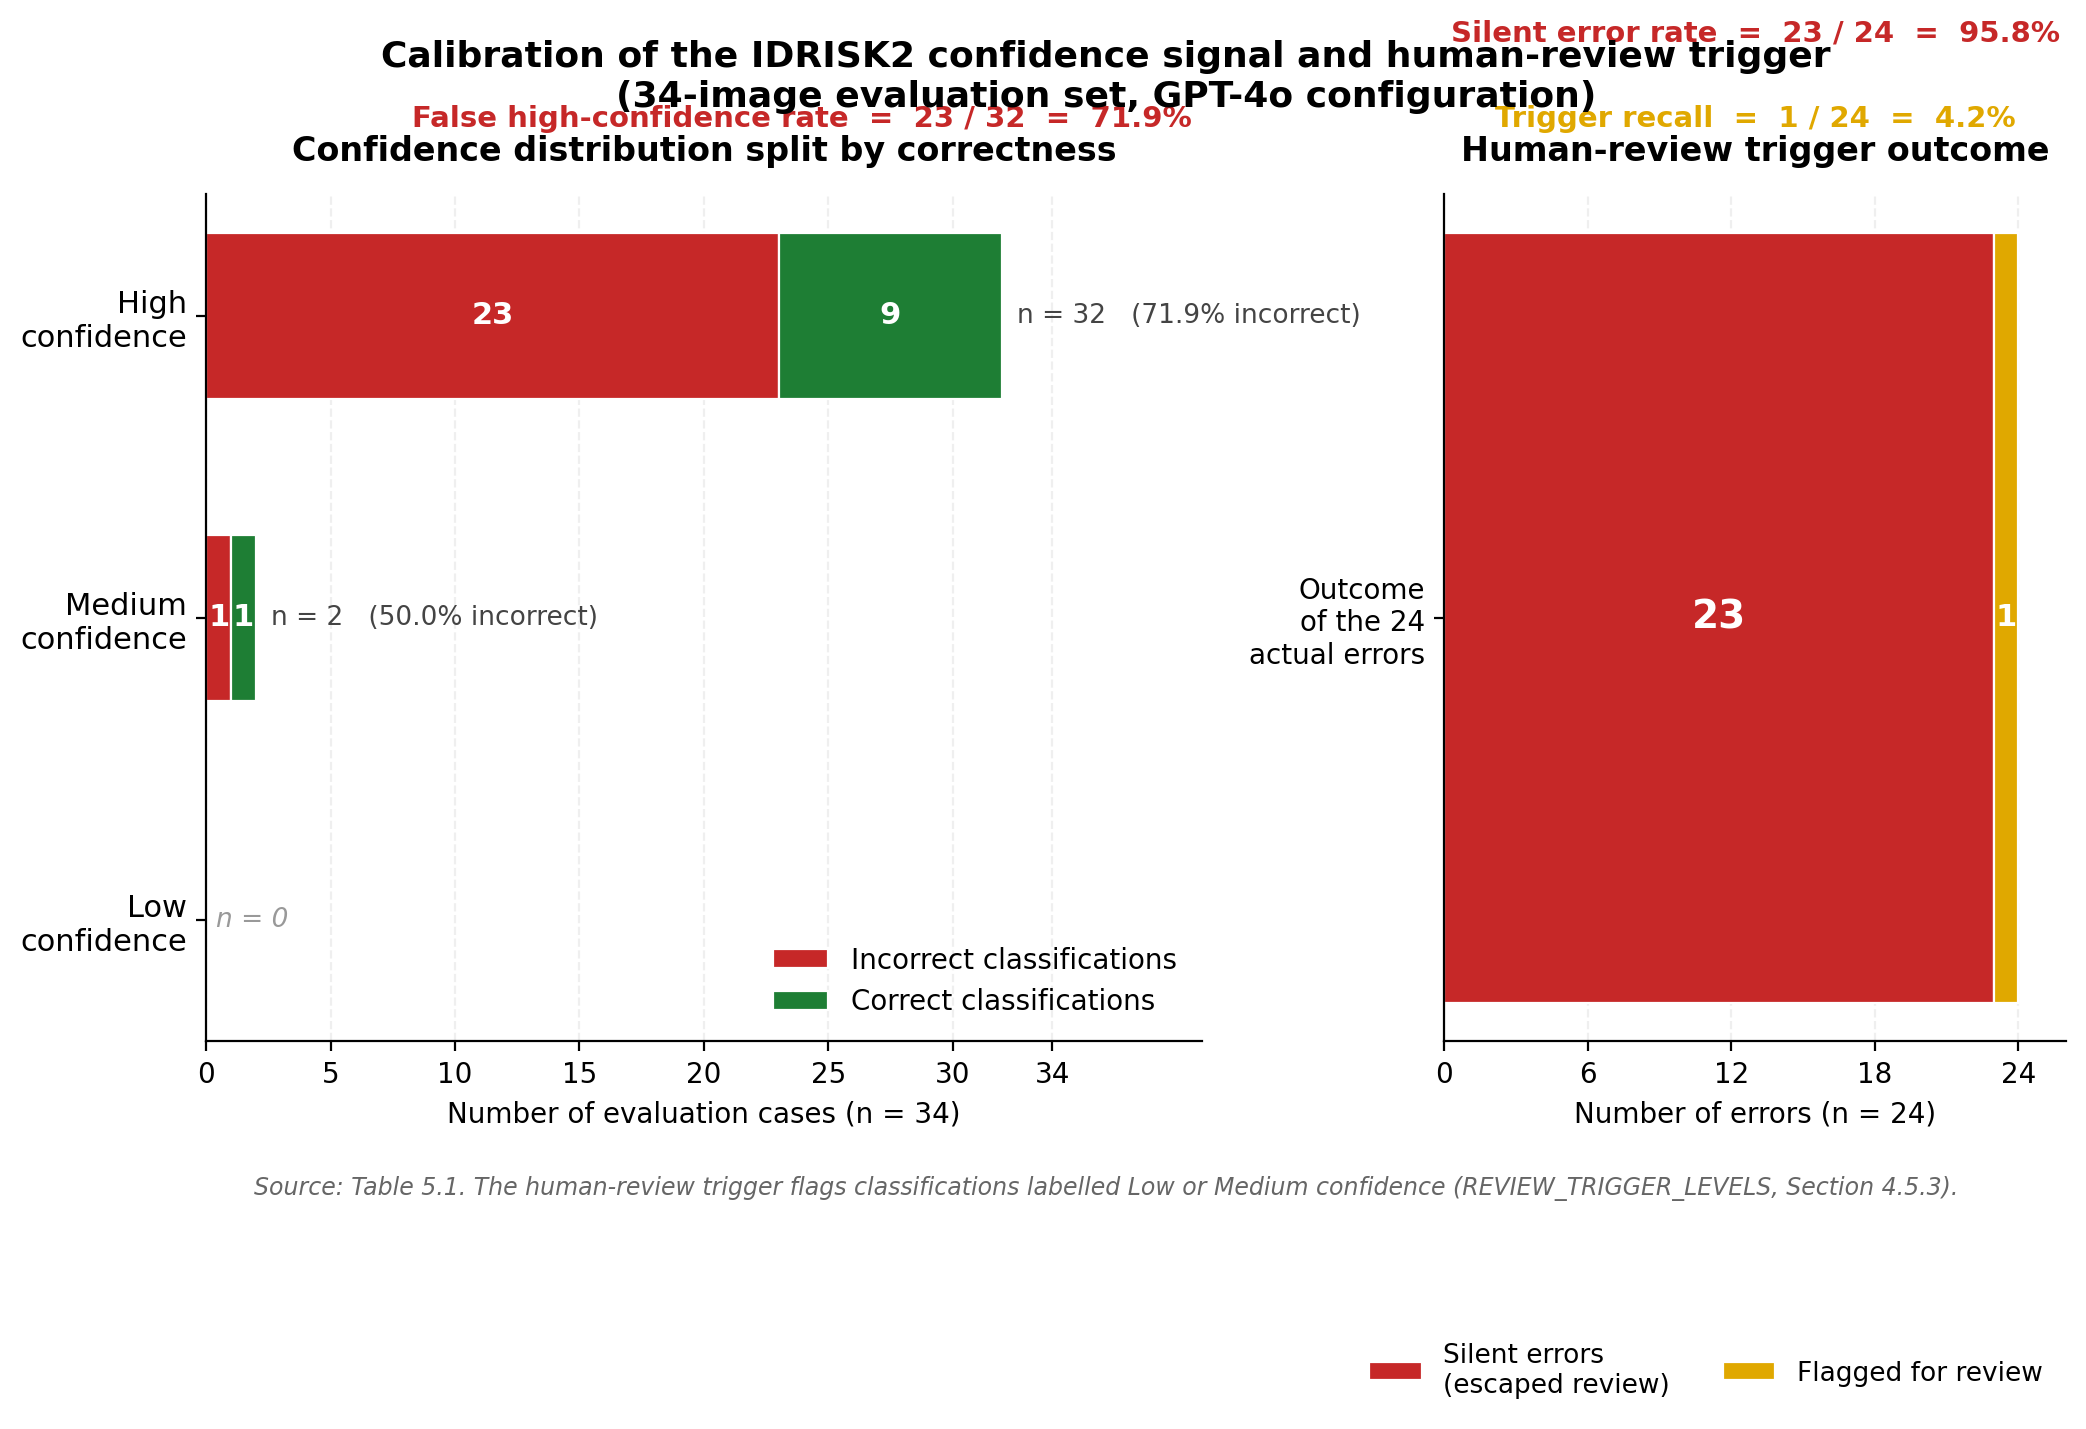
\includegraphics[width=0.85\linewidth,keepaspectratio]{fig4.png}
\caption{Calibration of the IDRISK2 confidence signal and the human-review trigger. The left panel partitions the 34 evaluation cases by the system's reported confidence level (32 high, 2 medium, 0 low) and splits each bucket by correctness against the ground truth; 23 of the 32 high-confidence outputs are incorrect, yielding a false high-confidence rate of 71.9\%. The right panel shows the outcome of the human-review trigger over the 24 actual errors: only 1 error (the medium-confidence mandioca case) was flagged for review, while 23 escaped review as silent errors, yielding a trigger recall of 4.2\% and a silent error rate of 95.8\%. These two values together quantify the calibration failure discussed in Sections 6.3 and 6.4 and motivate the trigger redesign proposed in Section 8.1.}
\end{figure}

\hypertarget{comparison-with-baseline-models}{%
\section{Comparison with Baseline Models}\label{comparison-with-baseline-models}}

\hypertarget{rag-augmented-system-versus-bare-vlm}{%
\subsection{RAG-augmented system versus bare VLM}\label{rag-augmented-system-versus-bare-vlm}}

The comparison between the bare VLM baseline and the full RAG-augmented system isolates the contribution of the retrieval and reranking layers. As reported in Sections 5.4 and 5.5, the VLM-only baseline achieves 0.0\% exact-match accuracy on the evaluation set; the RAG-augmented system achieves 29.4\%. The marginal contribution of the RAG layer is therefore +29.4 percentage points of exact-match accuracy and +58.8 percentage points of family-level accuracy. The retrieval and reranking layers are not a refinement of an already-functional baseline but the entire source of useful classification signal in the system.

\hypertarget{cross-vlm-comparison-proprietary-versus-open-source}{%
\subsection{Cross-VLM comparison: proprietary versus open-source}\label{cross-vlm-comparison-proprietary-versus-open-source}}

A cross-VLM comparison was conducted by re-running the full 34-image evaluation with the VLM stage substituted across three models, two proprietary, GPT-4o (OpenAI) and Claude Sonnet 4.6 (Anthropic), and one open-source 7B-parameter Vision-Language Model, LLaVA-NeXT-Mistral-7B, while holding the OCR, RAG, generation, and security stages of the pipeline constant. The objective of this comparison was twofold: first, to test the architectural claim of VLM substitutability documented in Section 6.2 against empirical data spanning the proprietary-versus-open-source dimension; and second, to determine whether the hallucination pattern characterised in Section 5.4 is a property of GPT-4o specifically, a property of the proprietary-VLM class, or a property of contemporary Vision-Language Models more generally. The complete set of comparative metrics is presented in Table 5.2 and visualised in Figure 5.2.

The two configurations yielded essentially convergent results on the headline metrics. The system's exact-match accuracy was 29.4\% under both VLMs (10 out of 34 images correctly classified); the false high-confidence rate was 71.9\% under GPT-4o and 69.7\% under Claude (a 2.2 percentage-point gap); and the silent error rate was 95.8\% under both. The two proprietary VLMs differ measurably on three secondary metrics. Family-level accuracy was 58.8\% under GPT-4o and 55.9\% under Claude, indicating that Claude's errors are marginally further from the ground truth taxonomy branch when they occur. Median per-image latency was 22.3 seconds under GPT-4o and 26.3 seconds under Claude, a difference of approximately 18\%. The mean rerank score of the top-1 candidate was 0.693 under GPT-4o and 0.720 under Claude, indicating slightly tighter top-of-list retrieval under the Claude configuration despite the equivalent end-to-end exact-match accuracy. The label-leak rate, defined in Section 5.5 as the proportion of cases in which the final classifier emits the VLM's preliminary code unchanged, was 11.8\% under GPT-4o (4 out of 34) and 23.5\% under Claude (8 out of 34), Claude approximately doubles the rate at which the final structured generator carries the VLM's preliminary code through to the output without validation against the retrieved candidate set.

Three findings of methodological significance arise from this comparison. First, the convergence of system exact-match accuracy at 29.4\% under two architecturally distinct proprietary VLMs constitutes the strongest available empirical evidence for the VLM-substitutability claim of Section 6.2: the choice between GPT-4o and Claude does not measurably affect the end-to-end accuracy that the RAG-augmented pipeline can achieve, which suggests that the determining factor in the system's accuracy is the retrieval and reranking stages rather than the upstream visual reasoning. Second, the convergence of the VLM-only baseline at 0.0\% across both proprietary models elevates the hallucination phenomenon from a GPT-4o-specific observation to a class-level property: a structured taxonomy classification at the granularity of FoodEx2 base terms appears to be a task on which contemporary proprietary VLMs systematically fail when evaluated in isolation, regardless of the specific model deployed. Third, the doubling of the label-leak rate under Claude indicates that the architectural defect documented in Section 5.5 is not uniformly distributed across VLMs but is sensitive to the verbosity and confidence with which the upstream VLM communicates its preliminary classification, a finding that strengthens the case for the output-validation mitigation proposed in Section 8.1.

Two additional observations are recorded for completeness. The convergence of the silent error rate at 95.8\% under both VLMs confirms that the human-review trigger calibration failure documented in Section 5.6 is a system-level defect arising from the confidence-only trigger design, not a property of the underlying VLM; substituting the VLM does not alleviate the calibration failure, which supports the redesign proposed in Section 8.1 as a precondition for Article 14 compliance independent of VLM choice. The 18\% latency penalty associated with Claude is well within operational tolerance for inspection workflows but is recorded here as evidence that VLM substitutability is an architectural property, not a free one: production deployments must price the latency differential when choosing between proprietary alternatives.

The substitution of the proprietary VLMs by the open-source LLaVA-NeXT-Mistral-7B model reveals the limits of the VLM-substitutability claim and provides a sharper empirical characterisation of where the architectural property breaks down. Under the LLaVA configuration, the system's exact-match accuracy collapses from 29.4\% to 2.9\% (1 of 34, the feijoada case, which the system classified correctly as A03VT "Beans, meat, and vegetables meal", a code that happens to coincide with the dish's literal description), and family-match accuracy falls from 58.8\% to 35.3\%. The bare-VLM exact-match accuracy remains at 0.0\%, consistent with both proprietary models, but the failure mode of the open-source VLM differs in character. LLaVA-NeXT produced the same preliminary code, A0FQJ "Mixed dish with meat and vegetables", in 33 of 34 cases, including for clearly distinct food categories such as brigadeiro (a chocolate confection), brownie (a chocolate cake), pastel de nata (a custard tart), pudim (a flan), guaraná (a canned soft drink), and tosta com avocado (a vegetarian toast). The VLM is therefore not producing diverse hallucinations across the test set, as the proprietary models do, but a single dominant generic-fallback hallucination repeated almost uniformly, which contaminates the RAG query with the same misdescription regardless of the actual visual content.

Three further LLaVA-specific findings carry methodological weight for the thesis. First, the label-leak rate under LLaVA is the lowest of the three VLMs at 8.8\%, lower than both GPT-4o (11.8\%) and Claude (23.5\%). This inversion appears counter-intuitive but follows directly from the homogeneity of LLaVA's hallucinated outputs: because the model nearly always proposes the same generic A0FQJ code, the retriever, the cross-encoder, and the LLM generator each have ample opportunity to override the proposal with a more specific candidate sourced from the retrieved context, and they do so in 31 of 34 cases. The label-leak metric, considered in isolation, would have misranked LLaVA as the most reliable of the three VLMs; the system-level exact-match accuracy reveals the contrary. This observation reinforces a methodological caution that label-leak is a diagnostic of VLM-classifier interaction, not a standalone quality indicator, and must be read jointly with downstream accuracy. Second, the system correctly emitted UNKNOWN with low confidence on two cases (hamburguer.jpg and ucal.jpg) under the LLaVA configuration, which produces a 5.9\% explicit-refusal rate not observed under the proprietary VLMs. The refusals coincide with cases where the retrieved candidate set offered no plausible match for the LLaVA-contaminated query, and the generator's instruction to ground every classification in retrieval correctly triggered a refusal rather than a fabrication. Third, the median per-image latency under LLaVA is 329 seconds, approximately 15 times that of GPT-4o, attributable to the local-inference cost of the 7B-parameter open-source model running with partial CPU offload on the Colab L4 GPU configuration documented in the appendix. This latency profile places the open-source configuration outside operational tolerance for time-sensitive inspection workflows under the current deployment hardware, although it remains tractable for batch reprocessing or offline annotation.

Together, the three-way comparison supports a refined version of the VLM-substitutability claim of Section 6.2. Substitutability holds robustly within the proprietary-VLM class for end-to-end accuracy, with secondary metrics that differ by single-digit percentage points. Substitutability does not hold between the proprietary-VLM class and the 7B open-source-VLM class evaluated here, where accuracy collapses by approximately one order of magnitude. The RAG layer continues to function under the open-source VLM, in the specific and weaker sense that it still overrides the VLM's preliminary code in 91.2\% of cases (the grounded-reasoning rate computed from the LLaVA run), but the corrections converge on a small set of dominant codes (A03VT in 19 of 34 cases) rather than on the dispersed correct codes that GPT-4o and Claude enable. The implication for deployment is that an open-source-only configuration is technically operable today, in the sense that it runs end-to-end and produces structured outputs with audit trails, but does not yet reach a useful accuracy threshold for regulatory-grade classification at this model scale. The position is recorded here as the empirical benchmark against which future open-source VLMs at larger parameter counts or with task-specific fine-tuning would need to be measured to demonstrate substantive convergence with the proprietary class.

\begin{longtable}[]{@{}llll@{}}
\toprule
\endhead
\textbf{Metric} & \textbf{GPT-4o} & \textbf{Claude Sonnet 4.6} & \textbf{LLaVA-NeXT 7B}\tabularnewline
Images evaluated (n) & 34 & 34 & 34\tabularnewline
System exact-match accuracy & 29.4\% (10/34) & 29.4\% (10/34) & 2.9\% (1/34)\tabularnewline
System family-match accuracy & 58.8\% (20/34) & 55.9\% (19/34) & 35.3\% (12/34)\tabularnewline
VLM exact-match accuracy & 0.0\% (0/34) & 0.0\% (0/34) & 0.0\% (0/34)\tabularnewline
Label-leak rate & 11.8\% (4/34) & 23.5\% (8/34) & 8.8\% (3/34)\tabularnewline
UNKNOWN refusal rate & 0.0\% (0/34) & 0.0\% (0/34) & 5.9\% (2/34)\tabularnewline
False high-confidence rate & 71.9\% & 69.7\% & 96.4\%\tabularnewline
Silent error rate (escaped review) & 95.8\% & 95.8\% & 81.8\%\tabularnewline
Median per-image latency & 22.3 s & 26.3 s & 329 s\tabularnewline
Mean rerank top-1 score & 0.693 & 0.720 & 0.659\tabularnewline
\bottomrule
\end{longtable}

\emph{Table 5.2, Cross-VLM comparison on the 34-image evaluation set across two proprietary VLMs (GPT-4o, Claude Sonnet 4.6) and the LLaVA-NeXT-Mistral-7B open-source baseline, with OCR, RAG, generation, and security stages held constant.}

\begin{figure}[htbp]
\centering
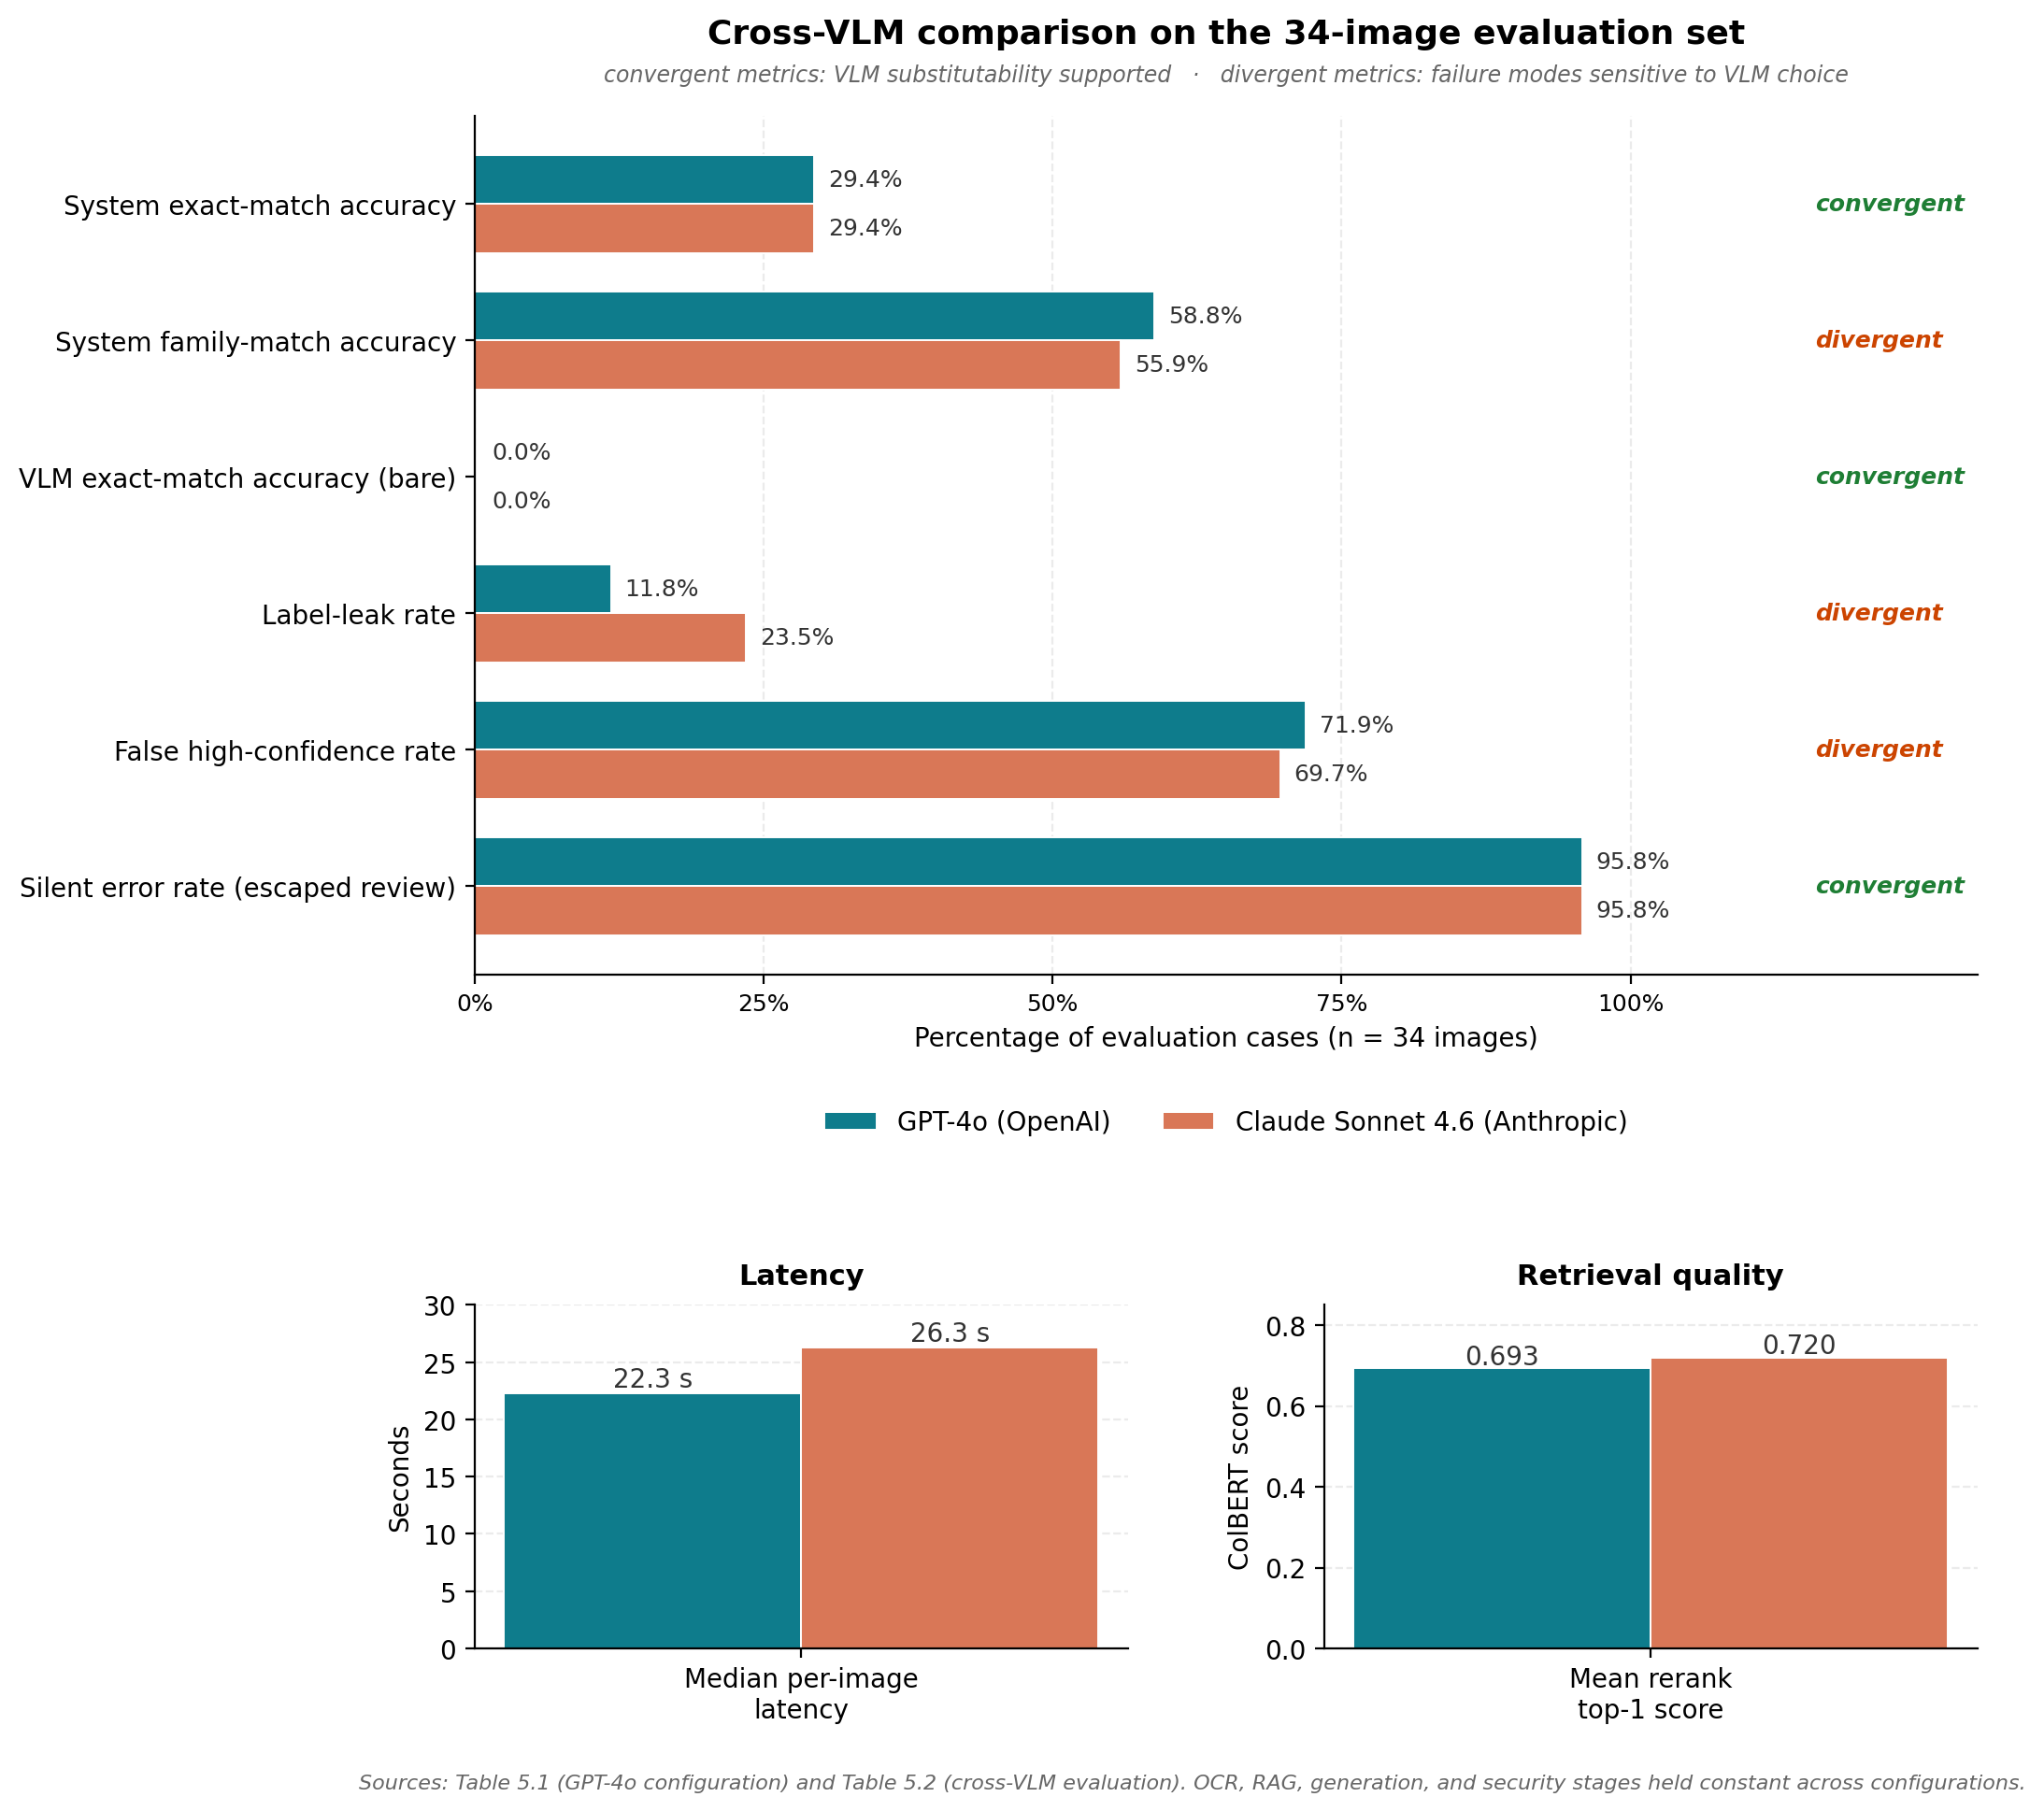
\includegraphics[width=0.85\linewidth,keepaspectratio]{fig5.png}
\caption{Cross-VLM comparison on the 34-image evaluation set across two proprietary VLMs (GPT-4o, Claude Sonnet 4.6) and the LLaVA-NeXT-Mistral-7B open-source baseline. The upper panel reports six percentage-based metrics; the proprietary-VLM pair converges on the headline accuracy and silent-error metrics, while the open-source 7B baseline collapses on system exact-match accuracy by approximately one order of magnitude, validates the bare-VLM zero-accuracy class-level property, and inverts the label-leak ordering by producing a single dominant generic-fallback hallucination across the test set. The lower panels report median per-image latency, where the LLaVA configuration is approximately 15 times slower than GPT-4o due to local 7B-parameter inference, and the mean rerank top-1 score, where retrieval quality degrades modestly under the homogeneous-query regime induced by the open-source VLM.}
\end{figure}

\hypertarget{output-stability-case-study}{%
\subsection{Output-stability case study}\label{output-stability-case-study}}

A third baseline comparison is implicit in the system's treatment of the dataset's three independent francesinha photographs. A robust classifier should assign identical or substantively equivalent codes to all three images of the same underlying dish. Under the GPT-4o configuration, the system assigned francesinha.jpg to A03ZB (correct), francesinha2.jpg to A040S "Pasta, cooked, with cheese/cream" (incorrect, assigning the dish to the pasta family), and francesinha3.jpg to A03XD "Meat loaf with cheese, vegetables or other" (incorrect, assigning to the meat-loaf family). Under the Claude configuration, the corresponding assignments were A03ZK, A03ZG, and A03ZB, all three within the sandwich (A03Z*) family but distinct sub-types, indicating that Claude exhibits visibly tighter family-level consistency on the controlled-stimulus subset even though only the third image reproduces the ground truth code. The variance of system output across visually equivalent inputs is therefore high enough under both VLMs that the same dish can be classified into three different specific codes depending on the photograph supplied, but the magnitude of the variance differs: GPT-4o crosses taxonomy families on this subset where Claude does not. This case is revisited in the detailed case-study analysis of Section 5.8.

\hypertarget{facet-level-classification-evaluation}{%
\subsection{Facet-level classification evaluation}\label{facet-level-classification-evaluation}}

The evaluations reported in Sections 5.7.1 through 5.7.3 measure the system's performance on the base term, the leftmost element of the FoodEx2 compound code (Section 2.1). A complete FoodEx2 classification, however, comprises the base term in combination with one or more facet descriptors, which encode orthogonal characterisation axes (part-nature, ingredient, process, packaging-format, packaging-material, and others, as documented in the FoodEx2 specification \parencite{european_food_safety_authority__efsa__200edd3d}, Section 5.7 and Appendix A). To assess the system's behaviour on the facet dimension of the classification task, a facet-level ground truth was constructed for the 34-image evaluation set covering the three facets the system most frequently emits across the cross-VLM comparison: F04 (Ingredient), F28 (Process), and, for the three packaged-drink items (guaraná, sumol, ucal) where they apply, F18 (Packaging-format) and F19 (Packaging-material).

The annotation methodology follows the FoodEx2 specification's guidance that F04 is a Repeatable facet whose focus should be the characterising ingredient of the food \parencite{european_food_safety_authority__efsa__200edd3d}. For each image, each relevant facet was annotated with a list of acceptable FoodEx2 codes drawn from the Appendix B taxonomy, allowing any one of the listed codes to count as correct under the per-image evaluation. For acarajé, for example, F04 was annotated as either A011Z "Beans (fresh seeds without pods) and similar" or A037N "Palm oil/fat", reflecting the two characterising ingredients of the dish; for chouriço, F04 was annotated as either A019L "Paprika powder" or A057F "Pig (as animal)", reflecting the spice that distinguishes chouriço from other cured sausages alongside the species of origin. Where a base term is sufficiently specific that a facet is implicit (Section 2.1; EFSA, 2015, Page 26), the facet is not annotated. The facet outputs emitted by each of the three evaluated VLMs (GPT-4o, Claude Sonnet 4.6, and LLaVA-NeXT-Mistral-7B) were extracted from the per-image results JSONL artefacts produced by the evaluation script and compared against this ground truth on three complementary metrics, coverage (the rate at which the system emits any value for a facet that the ground truth marks as relevant), accuracy-when-emitted (the rate at which an emitted value falls within the acceptable code list), and recall (the rate at which the system both emits a value and that value is acceptable, equivalent to the product of coverage and accuracy-when-emitted). A complementary aggregate score, the per-image facet hit rate, is also reported, defined as the fraction of the 34 images for which the system emitted at least one acceptable code across the set of relevant facets for that image. The full computation is implemented in data/evaluation/compute\_facet\_metrics.py and is deterministically reproducible from the evaluation JSONL artefacts and the facets\_gt entries of data/ground\_truth.json.

The cross-VLM results, reported in Table 5.3, identify three findings of methodological significance for the system's facet behaviour. The first is that the F18 and F19 packaging facets are emitted at a rate of 0.0\% across the three VLMs, despite three of the 34 images depicting clearly packaged beverages (a canned guaraná, a packaged sumol, and a tetra-pak ucal) for which these facets are unambiguously relevant. The architectural defect is not localised to any single VLM; it represents a systematic gap in the system's facet emission behaviour across all three configurations and is consistent with the absence of explicit packaging detection in the prompts used by the generation stage. The second finding is that F04 (Ingredient) is emitted at a high rate across all three VLMs (77.5\% to 94.1\% of relevant cases) but with low accuracy when emitted (11.5\% to 20.0\%), indicating that the system produces structurally well-formed facet outputs (the right slot is populated, with a code drawn from the FoodEx2 vocabulary) but the semantic content of those outputs is overwhelmingly incorrect. This is the facet-level analogue of the base-term hallucination phenomenon characterised in Section 5.4, and it confirms that the schema-validity-without-semantic-correctness failure mode is not restricted to the base term but extends across the compound classification.

The third finding is that F28 (Process) behaves substantially better than F04 and confirms the proprietary-to-open-source hierarchy established in Section 5.7.2 in a setting independent of the base term. Under GPT-4o, F28 is emitted in 65.5\% of relevant cases and is accurate when emitted in 63.2\% of those cases, yielding a recall of 41.4\%; under Claude, F28 is emitted in 82.8\% of cases but accurate in only 37.5\% (recall 31.0\%); under LLaVA-NeXT, F28 is emitted in 13.8\% of cases and accurate in 0.0\% of those (recall 0.0\%). The per-image facet hit rate aggregates these per-facet observations and follows the same pattern (GPT-4o 38.2\%, Claude 35.3\%, LLaVA-NeXT 8.8\%), recapitulating the order-of-magnitude collapse from proprietary to open-source 7B VLMs observed for the base term but at a different absolute scale: the proprietary VLMs converge near 35\% facet hit rate against a substantially lower exact-match accuracy on base term, indicating that the systems extract more useful descriptive information from the image than the base-term evaluation alone reveals. The implication for the system's operational deployment is that the facet dimension of the FoodEx2 classification carries useful signal under proprietary VLM configurations, even when the base term itself is incorrect, but does not extend gracefully to the open-source 7B class evaluated here.

\begin{longtable}[]{@{}llll@{}}
\toprule
\endhead
\textbf{Metric} & \textbf{GPT-4o} & \textbf{Claude Sonnet 4.6} & \textbf{LLaVA-NeXT 7B}\tabularnewline
Per-image facet hit rate (\textgreater=1 acceptable) & 38.2\% & 35.3\% & 8.8\%\tabularnewline
F04 (Ingredient), coverage & 88.2\% & 94.1\% & 76.5\%\tabularnewline
F04 (Ingredient), accuracy when emitted & 20.0\% & 18.8\% & 11.5\%\tabularnewline
F04 (Ingredient), recall & 17.6\% & 17.6\% & 8.8\%\tabularnewline
F28 (Process), coverage & 65.5\% & 82.8\% & 13.8\%\tabularnewline
F28 (Process), accuracy when emitted & 63.2\% & 37.5\% & 0.0\%\tabularnewline
F28 (Process), recall & 41.4\% & 31.0\% & 0.0\%\tabularnewline
F18 (Packaging-format), coverage & 0.0\% & 0.0\% & 0.0\%\tabularnewline
F19 (Packaging-material), coverage & 0.0\% & 0.0\% & 0.0\%\tabularnewline
\bottomrule
\end{longtable}

\emph{Table 5.3, Facet-level cross-VLM evaluation on the 34-image evaluation set. Coverage is the rate at which the system emits any value for a facet that the ground truth marks as relevant. Accuracy-when-emitted is the rate at which the emitted value falls within the acceptable code list for that facet. Recall is the product of coverage and accuracy-when-emitted. Per-image facet hit rate is the fraction of the 34 images for which at least one acceptable facet code was emitted across the relevant facet set. All values are deterministically reproducible from compute\_facet\_metrics.py.}

\hypertarget{case-studies}{%
\section{Case Studies}\label{case-studies}}

Five cases are selected as illustrative of the system's failure and success modes; each is briefly summarised here and developed further in the discussion.

The acarajé case (acaraje.jpg) is a cascading failure rooted in the VLM's visual misidentification. The model described the image as "fried plantains stuffed with shrimp and vegetables", visually plausible but factually wrong; acarajé is a fried fritter of black-eyed pea paste, not plantain. The query rewrite preserved this misidentification, the retriever surfaced vegetable-fried-dish candidates, and the final classifier assigned A03YC "Mixed vegetables, fried" with high confidence. The correct ground truth, A03VM "Legumes based dishes", was never present in the retrieved candidate set because the upstream query had been semantically contaminated by the VLM's initial error.

The sushi case (sushi.jpg) is an instance of label leak combined with retrieval failure. The VLM emitted the code A0C9N, officially "Young bulls (1-2 years) for dairy", together with the claimed label "Sushi". The retriever surfaced five sausage and surimi candidates, none of which were sushi. The final classifier nonetheless emitted A0C9N with the VLM's claimed label, despite the retrieval context offering no support for the assignment. The correct ground truth, A16GF "Rice, fish/seafood and vegetable based dishes", was not surfaced by the retriever and was not present in the final classifier's reasoning.

The salmão com arroz case (salmao\_com\_arroz.jpg) illustrates the human-review mechanism failing exactly when it would be most useful. The VLM mis-identified the image content as "chicken, avocado, sweet potatoes, greens" rather than salmon and rice. The system assigned A03VT "Beans, meat, and vegetables meal" with high confidence; the correct ground truth was A03XR "Fish and rice meal". Because the confidence was reported as high, the human-review trigger did not activate, and the error was emitted into the audit trail as a high-confidence classification.

The francesinha trio (francesinha.jpg, francesinha2.jpg, francesinha3.jpg) constitutes the dataset's controlled experiment on output stability. As reported in Section 5.7.3, the three images received entirely different classifications under the GPT-4o configuration, A03ZB (correct), A040S "Pasta, cooked, with cheese/cream", and A03XD "Meat loaf with cheese, vegetables or other", and three different sandwich-family classifications under the Claude configuration (A03ZK, A03ZG, A03ZB). The case demonstrates that the variance attributable to visual instability in the VLM stage is large enough to dominate the system's output even when the underlying food item is constant, and that the magnitude of the variance is sensitive to VLM choice: GPT-4o crosses taxonomy families on this controlled stimulus subset where Claude does not.

The brigadeiro case (brigadeiro.jpg) is a clean success: the VLM produced the hallucinated code A0D7F ("Lime infusion flowers and similar") but the RAG retriever surfaced A034R "Chocolate coated confectionery" as the top reranked candidate, the LLM generator selected it correctly, and the system emitted A034R with high confidence and reasoning grounded in the retrieved passage. The case demonstrates the system functioning as designed, with the retrieval layer correctly overriding a hallucinated VLM proposal.
  % Evaluation and Results
\hypertarget{discussion}{%
\chapter{Discussion}\label{discussion}}

This chapter interprets the empirical findings of Chapter 5 in the context of the broader research questions identified in Chapter 1 and the literature reviewed in Chapter 3. The discussion is organised around six interpretive lenses: the consolidation of the key quantitative findings into a coherent claim about the system's behaviour (6.1), the architectural strengths that the evaluation supports (6.2), the challenges encountered and the specific design decisions taken to address them (6.3), the implications of the results for food safety practice and regulatory compliance (6.4), the comparative position of the IDRISK2 system relative to the state of the art (6.5), and an honest accounting of the limitations of the current evaluation (6.6).

\hypertarget{interpretation-of-key-findings}{%
\section{Interpretation of Key Findings}\label{interpretation-of-key-findings}}

The single most consequential finding of the evaluation is that the IDRISK2 system's classification accuracy is entirely attributable to the Retrieval-Augmented Generation layer. The Vision-Language Model, evaluated in isolation, produced zero correct base-term assignments across 34 images; the full RAG-augmented pipeline produced 10 correct assignments and 20 family-level assignments. The marginal contribution of the retrieval and reranking stages is therefore not an incremental improvement over a baseline but the entire useful signal of the system. This result transforms the methodological status of the RAG architecture from an enhancement to a necessary precondition for the system's existence as a regulatory-grade classifier.

The pattern of VLM failures provides a fine-grained characterisation of the hallucination phenomenon in the structured-taxonomy domain. The model did not produce malformed outputs: every preliminary code conformed to the FoodEx2 syntactic format of an A-prefix followed by four alphanumeric characters, and every accompanying natural-language description of the image was substantively accurate. The failure mode is specifically the binding between visual content and taxonomy identifier, where the model lacks reliable parametric knowledge of the 31,303-term taxonomy and resorts to plausible-looking fabrications. The recurrence of a small set of codes as fallbacks (A0FQJ five times, A0EKC four times) is consistent with the model having memorised a handful of FoodEx2-shaped strings during training and reusing them as generic answers when no confident parametric mapping exists. Crucially, these fabrications are emitted with high confidence in 33 of 34 cases, which renders the confidence signal of the upstream VLM useless for any downstream calibration purpose.

The cross-VLM evaluation reported in Section 5.7.2 strengthens this characterisation from a single-model observation to a class-level claim, and further refines it through comparison with the open-source 7B-parameter alternative. When the same 34-image dataset is processed with Claude Sonnet 4.6 instead of GPT-4o, the bare-VLM exact-match accuracy remains at 0.0\% and the end-to-end system accuracy remains at 29.4\%; the two proprietary VLMs converge on identical headline metrics. When the substitution extends to LLaVA-NeXT-Mistral-7B, the bare-VLM exact-match accuracy remains at 0.0\% but the end-to-end system accuracy collapses to 2.9\%. The triple convergence of the bare-VLM result at zero across architectures of widely differing parameter count and training regime makes the hallucination phenomenon a property of the contemporary Vision-Language Model class as a whole, not a quirk of any single model nor of the proprietary subclass; it elevates the methodological status of the retrieval-grounded correction from a useful mitigation to an empirically necessary one across the available alternatives. The same comparison delimits the architectural substitutability of the VLM layer that Section 6.2 had previously characterised as a design-time property: substitutability holds robustly within the proprietary class, where GPT-4o and Claude yield equivalent system accuracy, but breaks down at the proprietary-to-7B-open-source boundary, where system accuracy drops by an order of magnitude. The determining factor in system accuracy is therefore the joint quality of the VLM's preliminary signal and the retrieval and reranking stages downstream of it, not either component in isolation.

Conversely, the pattern of RAG successes confirms the design choice documented in Section 4.5.1 to index the FoodEx2 taxonomy at term granularity rather than as further-chunked passages. In every classification, all five retrieved candidates were atomic taxonomy term nodes, and the LLM-based generator selected from this candidate set in the 30 cases that did not exhibit label leak. The brigadeiro case study in Section 5.8 is the cleanest instance of this dynamic: the VLM proposed a hallucinated code in the unrelated taxonomic family of "Lime infusion flowers", but the retriever surfaced "Chocolate coated confectionery" as the top reranked candidate, and the generator correctly overrode the VLM's proposal. The RAG layer, in this functioning regime, operates exactly as the literature on hallucination mitigation predicts: by replacing parametric guessing with verifiable evidence retrieval.

The family-level accuracy of 58.8\% relative to the exact-match accuracy of 29.4\% indicates that the dominant residual failure mode of the system, after the RAG correction takes effect, is granularity selection within the correct hierarchy branch rather than gross taxonomic misclassification. Of the 24 cases where the system did not exactly match the ground truth, 10 fell within the same three-character taxonomy prefix as the ground truth and 14 did not. The granularity errors are typically distinctions that a non-expert human annotator would also find difficult, for example A00BG "Chocolate cake" versus A00BF "Chocolate-based cakes" for the brownie image, or A025N "Sliceable or firm cooked sausages" versus A025C "Chorizo and similar" for the chouriço image. These are tractable improvements through better prompting and richer term descriptions in the indexed corpus. The remaining 14 cases of cross-family error are the substantively harder problem and motivate the architectural changes proposed in Section 8.1.

\hypertarget{advantages-of-the-proposed-idrisk2-system}{%
\section{Advantages of the Proposed IDRISK2 System}\label{advantages-of-the-proposed-idrisk2-system}}

The evaluation supports three architectural choices made in the system's design. The first is the decision to combine the EFSA technical PDFs with the Appendix B taxonomy XLSX as two complementary indexing streams with heterogeneous chunking strategies. The PDFs supplied governance and methodology context useful for grounding generation, while the atomic taxonomy term nodes supplied the candidate identifiers that the classifier required to produce correct outputs. The cross-encoder consistently reranked term nodes above PDF chunks across all 34 evaluations, which validates the heterogeneous-chunking design: the choice to leave each taxonomy term as an unfragmented atomic node preserves the semantic locality that the reranker depends on, and the choice to chunk PDFs semantically preserves the descriptor definitions intact for the generation context.

The second supported choice is the use of an Advanced RAG architecture combining pre-retrieval query rewriting, HyDE-based dense retrieval, sparse BM25 lexical retrieval, Reciprocal Rank Fusion, and ColBERT cross-encoder reranking. The mean top-1 rerank score of 0.693 is substantially above the 0.611 ceiling observed in earlier pilot runs that indexed only the EFSA PDFs, confirming the value of the layered retrieval pipeline. The fact that 100\% of retrieved candidates were taxonomy terms across all evaluations indicates that the cross-encoder discriminates effectively between meta-level documentation and dish-level taxonomy entries, which is the discrimination most directly relevant to classification.

The third supported choice is the closed, self-hosted deployment architecture documented in Section 4.6. The BAAI/bge-m3 embedding model, the Chroma vector store, the cross-encoder reranker, and the rule-based security infrastructure all operate locally on infrastructure controlled by the deploying organisation. Only the calls to the proprietary VLM (GPT-4o or Claude, depending on configuration) exit the deployment boundary; the architecture supports substitution of either proprietary VLM by an open-source LLaVA-NeXT deployment at the cost of additional local compute and the loss of state-of-the-art reasoning quality. This design preserves the option for fully self-hosted operation as the open-source VLM ecosystem matures, without requiring re-architecting of the retrieval or generation layers.

Beyond accuracy considerations, the evaluation supports the operational feasibility of the system. The median latency of 22.3 seconds with a standard deviation of 1.5 seconds across heterogeneous inputs indicates predictable per-classification cost, which is a precondition for inclusion in time-sensitive inspection workflows. The audit trail produced by every classification, comprising the cryptographically chained HMAC entries written by the AuditLogger and the per-decision provenance records written by the generation component, provides the documentation required by the EU AI Act for high-risk AI systems, regardless of the classification's correctness. The system therefore meets the documentation and traceability obligations of the regulatory framework even where it fails to meet the accuracy obligations, which is an important separation for deployment in supervised regulatory contexts.

\hypertarget{challenges-encountered-and-solutions-adopted}{%
\section{Challenges Encountered and Solutions Adopted}\label{challenges-encountered-and-solutions-adopted}}

Four substantive architectural challenges emerged during the development and evaluation of the system. Each is documented here with the design response adopted and the residual risk that remains for future iterations.

The first challenge is the label leak phenomenon observed in 4 of 34 cases under the GPT-4o configuration (11.8\% of the evaluation set), 8 of 34 cases under the Claude configuration (23.5\%), and 3 of 34 cases under the LLaVA-NeXT-7B configuration (8.8\%). When the VLM emits a preliminary FoodEx2 code together with a fabricated natural-language label, the final structured generator can carry both the code and the label through to its output even when the retrieved context does not support the assignment. This failure mode arises because the generation prompt presents both the VLM's preliminary classification and the retrieved candidates as joint context, and the LLM occasionally treats the VLM's claim as a permitted continuation rather than a hypothesis to be checked against retrieval. The mitigating design response is the explicit instruction in the generation system prompt to base classification decisions "only on the retrieved documentation provided" (Section 4.5.3). The interpretation of the leak rate must be read jointly with downstream accuracy. Under the open-source LLaVA configuration the leak rate is the lowest of the three VLMs, but this apparent advantage is the symptomatic outcome of LLaVA's near-uniform emission of a single generic-fallback code (A0FQJ "Mixed dish with meat and vegetables" in 33 of 34 cases), which the retriever and the cross-encoder readily override, rather than evidence of strong VLM-classifier discipline. The leak metric therefore diagnoses VLM-classifier interaction and is not a standalone quality indicator. The residual risk is documented as an architectural defect requiring a downstream validation step in which the emitted code must be verified against the retrieved candidate set before the output is returned; the cross-VLM evidence strengthens the case for this mitigation by demonstrating that VLM substitution alone does not eliminate the failure mode, that under some VLM choices it amplifies it (Claude), and that under others it merely shifts the dominant failure mode from leak to retrieval contamination (LLaVA).

The second challenge is the cultural-coverage limitation of the FoodEx2 taxonomy itself. The dataset's emphasis on Portuguese and Brazilian dishes surfaced repeated cases in which no specific term exists for the food being classified: acarajé (no specific code, mapped to "Legumes based dishes"), brigadeiro (no specific code, mapped to "Chocolate coated confectionery"), pastel (no specific code, mapped to "Sandwiches, pizza and other stuffed bread-like cereal products"), rabanada (no specific code, mapped to the generic base term "Wheat bread and rolls, white"), and the Brazilian cuscuz nordestino (no specific code, mapped to the structurally similar "Couscous" entry derived from Maghrebi cuisine). This is a coverage limitation of the EFSA taxonomy rather than a defect of the IDRISK2 system, but it materially affects the achievable accuracy ceiling on the Lusophone evaluation set. The mitigating response, adopted at ground-truth annotation time, was to apply the FoodEx2-prescribed practice of selecting the closest generic base term and intending that the dish-specific characterisation be carried by facets. The residual risk is that the system's outputs in these cases convey less information than a Brazilian or Portuguese inspector would expect, which raises an open question about whether the European-centric taxonomy is appropriate as the unique target ontology for inspection workflows in Brazil and Portugal.

The third challenge is the cascading failure pattern observed when the upstream VLM misidentifies the visual content of the image. The acarajé case discussed in Section 5.8 is the prototypical example: a single error in the VLM's visual description ("fried plantain" instead of "fried bean fritter") propagates through query rewriting, HyDE generation, retrieval, and reranking, with each downstream stage operating faithfully on the contaminated input. The system's modular design treats each stage as a trusted producer for the next, and there is no mechanism to detect or rollback an upstream error. The mitigating response adopted in the current architecture is the chain-of-thought reasoning field in the structured generation output, which produces a human-readable record of the system's classification rationale that an auditor can inspect after the fact. The residual risk is that errors of this category are not detected automatically and that their detection depends on human review, which the evaluation showed to be ineffective at 4.2\% recall on actual errors.

The fourth challenge is the calibration of the system's confidence signal. The evaluation revealed a false high-confidence rate of 71.9\% and a silent error rate of 95.8\%, figures that establish the current confidence mechanism as effectively non-functional for regulatory purposes. The mitigating design response was the introduction of the configurable REVIEW\_TRIGGER\_LEVELS policy (Section 4.5.3) that flags any classification with low or medium confidence for human review by default. This policy correctly triggered review on 2 of the 34 evaluations, but in only one case (mandioca) was the flagged classification incorrect, while 23 incorrect classifications passed through with high confidence and no flag. The residual risk is substantial: under the current policy, the human-review mechanism does not satisfy the human-oversight obligation of EU AI Act Article 14 for high-risk AI applications, and the architectural redesign of the trigger is documented as priority future work in Section 8.1.

\hypertarget{implications-for-food-safety-and-compliance}{%
\section{Implications for Food Safety and Compliance}\label{implications-for-food-safety-and-compliance}}

The deployment of the IDRISK2 system as an autonomous classifier is not supported by the current evaluation. An exact-match accuracy of 29.4\% combined with a 71.9\% false high-confidence rate places the system far below the threshold at which automatic classifications could replace human judgement in a regulatory food-safety workflow. The implication for deployment is therefore that the system, in its present configuration, must operate as a decision-support tool with mandatory human review on every classification, not only on those flagged by the automatic trigger. This reverses the implicit assumption of the architecture, in which review is the exception rather than the rule, and brings the operational practice into line with the calibration that the evaluation has actually measured.

Under that revised deployment model, the system's contribution to inspection workflows is best framed as the production of a high-quality candidate classification and a complete audit trail, both of which are presented to a human inspector for final adjudication. In this framing, the family-level accuracy of 58.8\% is more directly relevant than the exact-match accuracy: 58.8\% of the time, the system places the inspector within the correct three-character branch of the taxonomy and reduces the search space for human review from 31,303 terms to a small set of related candidates. The inspector retains responsibility for the final code selection, the system's confidence signal becomes an advisory rather than authoritative input, and the audit trail produced by every classification supports post-hoc review by supervisors or auditors. This framing is consistent with the human-in-the-loop deployment model recommended for high-risk AI systems by the EU AI Act and is the model the IDRISK2 system can support today. The web frontend described in Section 4.8 was designed against this deployment model: the role-specific screens surface the candidate classification, the live pipeline progress, and the audit trail to the inspector and supervisor at the appropriate points in the workflow, while the human-review queue on the supervisor dashboard materialises the human-oversight mechanism on which the EU AI Act compliance posture depends.

With respect to the GDPR, the system's compliance posture is robust. The closed deployment architecture documented in Section 4.6 keeps all product data on infrastructure controlled by the deploying authority, the data-minimisation mechanism discards raw image bytes immediately after feature extraction and persists only the SHA-256 hash and the classification result, and the chained HMAC audit log provides the tamper-evident traceability required by Article 22 for automated decision-making. The label leak phenomenon discussed in Section 6.3 is, in this context, a defect specifically of explainability: when the system emits a label that does not correspond to the official taxonomy entry for the assigned code, the audit record contains a misleading rationale that cannot be unambiguously reconciled with the FoodEx2 ground truth. This is a tractable defect, adding a final validation step that resolves every emitted code against the taxonomy and rejects mismatches, but its mitigation is required before the system can claim full compliance with the explainability obligations of Article 22.

With respect to the EU AI Act, the system's current calibration failure is the dominant compliance gap. Article 14's human-oversight requirement presupposes a meaningful trigger that escalates uncertain decisions to human review; a trigger that captures 4.2\% of actual errors does not meet this presupposition. The deployment posture proposed above, mandatory human review on every classification, sidesteps the calibration problem by removing the system's discretion to release outputs without review, at the cost of reducing the system's labour-saving value. The architectural redesign of the trigger, with which the system could plausibly operate with the automatic-review-by-exception posture originally intended, is identified as a precondition for full Article 14 compliance and is developed as future work in Section 8.1.

\hypertarget{comparison-with-state-of-the-art}{%
\section{Comparison with State-of-the-Art}\label{comparison-with-state-of-the-art}}

A direct quantitative comparison between the IDRISK2 system and the prior state of the art in automated FoodEx2 classification is constrained because the most advanced existing system, FEAST \parencite{lorenzo_molfetta_47d7c4cd}, operates on a fundamentally different input modality. FEAST consumes pre-structured textual food descriptions and produces multi-hierarchical FoodEx2 classifications through a retriever-reranker architecture; it does not ingest images. The 34-image dataset used in the present evaluation cannot be passed to FEAST without an upstream description-generation step, which is precisely the role that the OCR-and-VLM stages of the IDRISK2 system perform. The two systems address different points on the same end-to-end pipeline: FEAST is the textual-description-to-FoodEx2 specialist that the IDRISK2 system's RAG layer is broadly an instance of, while the IDRISK2 system as a whole is the image-to-FoodEx2 generalist that includes a FEAST-like component as its terminal stage.

The implication of this architectural separation is that the IDRISK2 system addresses the harder problem and accepts a correspondingly lower accuracy as the price of taking real-world inputs. The 29.4\% exact-match accuracy reported in Section 5.6 reflects the compounded error of the upstream VLM (which introduces visual misidentification, hallucinated codes, and contaminated queries) before any taxonomy-classification step has begun. The substantially higher accuracy reported by FEAST on structured-text inputs \parencite{lorenzo_molfetta_47d7c4cd} is not directly comparable because those figures measure the accuracy of the taxonomy-classification step in isolation, downstream of an assumed-correct textual description, whereas the IDRISK2 figure measures the end-to-end accuracy from raw image input. A faithful comparison would require either deploying FEAST on the VLM-generated descriptions produced by the IDRISK2 pipeline (which would introduce a stack-mismatch evaluation) or constructing a parallel dataset of textual descriptions that bypasses the visual stage entirely (which would not exercise the IDRISK2 system's core contribution).

The IDRISK2 system's specific contribution relative to the state of the art is therefore the demonstration of the end-to-end image-to-FoodEx2 pipeline on real-world dish photographs, complete with the closed-deployment, GDPR-compliant, EU AI Act-aware infrastructure that the literature reviewed in Section 3.5 identified as missing from existing approaches. The accuracy of the system is lower than what a structured-text classifier could achieve on cleaner inputs, but the system addresses an operational scenario, point-of-sampling classification by inspectors using smartphone photographs, that no published prior system has covered. The four gaps identified in Section 3.5 (end-to-end image-to-FoodEx2 pipeline, VLM evaluation on FoodEx2 classification, regulatory compliance integration, and closed self-hosted deployment) are addressed by the IDRISK2 system, even where the accuracy of the present implementation falls short of operational sufficiency.

\hypertarget{limitations-of-the-current-study}{%
\section{Limitations of the Current Study}\label{limitations-of-the-current-study}}

The evaluation reported in Chapter 5 is subject to five limitations that must be carried forward into the interpretation of the findings and the planning of future work.

First, the dataset size of 34 images is small for an empirical evaluation of an AI system. The reported accuracy and calibration figures have wide statistical uncertainty: an exact-match accuracy of 10/34 has a 95\% confidence interval of approximately 16\% to 47\%, and the 4 label-leak cases observed in the evaluation could plausibly correspond to a population rate anywhere between 3\% and 27\%. The qualitative findings, that the VLM hallucinates structurally, that the RAG layer is the source of all useful accuracy, that the calibration signal is uninformative, are robust to this uncertainty because they arise from patterns rather than precise percentages, but the specific numerical claims should be interpreted as point estimates with wide intervals. A larger evaluation set, ideally several hundred images, would be required to fix the metrics with the precision that would support deployment decisions.

Second, the ground truth was assigned by a single annotator. Inter-annotator agreement on FoodEx2 classification of culturally specific dishes is itself an open question, and the present evaluation cannot distinguish between cases where the system disagreed with the ground truth and cases where two annotators might have disagreed about the ground truth. The decision to record the system's family-level accuracy alongside its exact-match accuracy was motivated in part by this concern: the family-level metric is robust to disagreements between annotators about the specific sub-type within an agreed-upon family. Future work should include a multi-annotator validation on at least a subset of the evaluation set, with Cohen's Kappa or Fleiss's Kappa reported as a measure of the agreement ceiling against which the system's accuracy should be evaluated.

Third, the dataset is biased toward Portuguese and Brazilian dishes, which oversamples the cultural-coverage gap of the FoodEx2 taxonomy discussed in Section 6.3. A more representative dataset spanning the full geographical scope of EFSA's regulatory remit would be needed to estimate the system's accuracy in the operational European context. The bias is, however, deliberate for the purposes of the present evaluation, which aimed specifically to expose the system to inputs that would stress its coverage and grounding properties. The reported accuracy figures should therefore be read as a lower-bound estimate of what the system would achieve on a European-balanced dataset, not as a representative central estimate.

Fourth, the VLM evaluation reported in this dissertation covered all three interchangeable VLM backends supported by the system (Section 4.4.1): GPT-4o (OpenAI), Claude Sonnet 4.6 (Anthropic), and LLaVA-NeXT-Mistral-7B \parencite{liu_llava_next_2024}, all reported in Section 5.7.2. The included open-source evaluation establishes the boundary of the substitutability claim of Section 6.2 at the proprietary-to-7B-open-source transition and quantifies the accuracy collapse that results, but the open question of whether other contemporary open-source VLMs of comparable scale would reproduce the same failure profile, or whether the LLaVA-specific generic-fallback regime is idiosyncratic, remains formally open. A further open question is whether an instruction-tuned open-source VLM at a larger parameter count, or one fine-tuned on FoodEx2 documentation and labelled food imagery, could reduce the hallucination rate observed at 7B scale at the price of higher local compute cost. The cross-VLM evidence reported in Section 5.7.2 already supports the architectural substitutability claim within the proprietary class and refutes it at the proprietary-to-7B-open-source boundary; broader confirmation against additional open-source families and larger parameter counts is identified as follow-up work in Section 8.1.

Fifth, the efficiency criterion of the central research question (Section 1.3) is only partially addressed by the present evaluation. The system's per-image latency was measured (median 22.3 seconds, standard deviation 1.5 seconds) and the reduction of the inspector's effective search space from 31,303 taxonomy terms to a five-candidate reranked set was quantified, both of which characterise the system's intrinsic computational behaviour. What was not measured, and what the efficiency criterion strictly requires, is a comparative A/B evaluation against the current manual classification workflow with quantified end-to-end inspector throughput, time-to-classification, and cognitive load. The claim that the system improves the efficiency of FoodEx2 coding therefore rests on the latency and search-space-reduction indicators as preconditions for efficiency gains, rather than on a directly measured efficiency differential. The A/B field study required to quantify the efficiency differential is identified as a longitudinal-study priority in Section 8.5.
  % Discussion
\hypertarget{conclusion}{%
\chapter{Conclusion}\label{conclusion}}

This dissertation proposed and evaluated IDRISK2, an end-to-end pipeline for the automated assignment of FoodEx2 classification codes to food images, combining optical character recognition, vision-language reasoning, and a retrieval-augmented generation layer grounded in the official EFSA FoodEx2 taxonomy. This concluding chapter summarises the research carried out, the contributions it makes to the field, and the closing reflections that arise from the evaluation.

\hypertarget{summary-of-research}{%
\section{Summary of Research}\label{summary-of-research}}

The research was motivated by the persistent difficulty of mapping food product information to FoodEx2 codes in a regulatory inspection context. Manual classification is time-consuming, error-prone, and creates a bottleneck for downstream risk assessment by EFSA. Recent advances in vision-language and retrieval-augmented architectures opened the possibility of automating this mapping, but no existing system had been demonstrated end-to-end from real-world product imagery to compliant FoodEx2 outputs within a closed deployment environment aligned with GDPR and EU AI Act requirements. The central research question formulated in Section 1.3 asked how the integration of computer vision, OCR, and retrieval-augmented language models could improve the efficiency, accuracy, and security of FoodEx2 coding while remaining compliant with the cybersecurity requirements of ASAE, SIT, and FVST.

To address that question, Chapter 4 specified a modular pipeline comprising five processing layers: image preprocessing and OCR (Sections 4.2 and 4.3), vision-language interpretation (Section 4.4), Advanced RAG retrieval over a knowledge base built from the EFSA technical PDFs and the Appendix B taxonomy XLSX (Sections 4.5.1 and 4.5.2), structured FoodEx2 generation with audit logging (Section 4.5.3), and a closed security and compliance layer enforcing role-based access control, data minimisation, and tamper-evident audit chaining (Section 4.6). The implementation was evaluated empirically on 34 photographs of culturally specific dishes and packaged products, against a manually annotated FoodEx2 ground truth, and the results were reported in Chapter 5.

The evaluation established four substantive findings. First, the Vision-Language Model produces preliminary FoodEx2 codes that are structurally well-formed but semantically fabricated in 100\% of evaluations, with hallucinated identifiers presented at high confidence. Second, the RAG retrieval and reranking layers correct these hallucinations and contribute the entirety of the system's useful classification accuracy, achieving 29.4\% exact-match and 58.8\% family-level accuracy. Third, the system's confidence signal does not track actual correctness, with a false high-confidence rate of 71.9\% and a silent error rate of 95.8\% that materially weakens the human-oversight mechanism. Fourth, the closed deployment architecture, the data-minimisation pipeline, and the cryptographically chained audit log satisfy the explainability and traceability requirements of GDPR Article 22 and the documentation obligations of the EU AI Act for high-risk AI systems, even where the system's accuracy and calibration fall short of fully autonomous deployment.

\hypertarget{contributions-to-the-field}{%
\section{Contributions to the Field}\label{contributions-to-the-field}}

Relative to the four gaps identified in Section 3.5, this work makes the following contributions.

First, this dissertation presents the first end-to-end pipeline reported in the literature that ingests raw food product imagery, as captured under real-world inspection conditions, and produces structured FoodEx2 classifications grounded in the official EFSA taxonomy. The most advanced prior system, FEAST \parencite{lorenzo_molfetta_47d7c4cd}, operates on pre-structured textual food descriptions and does not address the upstream visual-interpretation problem; the IDRISK2 system covers the entire stack from photograph to compliant code assignment.

Second, this dissertation contributes the first systematic empirical evaluation of Vision-Language Model behaviour on FoodEx2 classification, spanning the proprietary-versus-open-source dimension and covering both the base term and the facet dimensions of the compound classification. The finding that GPT-4o, the strongest available proprietary VLM at the time of writing, achieves zero exact-match accuracy and emits hallucinated taxonomy codes in 100\% of cases (94\% misattributed real codes plus 6\% non-existent codes), and that this zero-accuracy result reproduces under Claude Sonnet 4.6 and under the LLaVA-NeXT-Mistral-7B open-source baseline, elevates the hallucination phenomenon from a single-model observation to a class-level property of contemporary Vision-Language Models on structured-taxonomy classification tasks. The complementary finding that the RAG layer compensates for this VLM failure to recover 29.4\% exact-match accuracy under the proprietary VLMs but only 2.9\% under LLaVA-NeXT-7B delimits the empirical boundary at which proprietary-to-open-source VLM substitutability breaks down for this task, at approximately one order of magnitude of system accuracy. The facet-level evaluation reported in Section 5.7.4 extends this characterisation to the descriptive dimension of the FoodEx2 code, documenting that the same proprietary-versus-open-source ordering reproduces (per-image facet hit rate of 38.2\% for GPT-4o, 35.3\% for Claude, 8.8\% for LLaVA-NeXT-7B) and identifying two architectural defects of independent interest, the systematic non-emission of the packaging-format and packaging-material facets (0.0\% coverage across all three VLMs even on relevant packaged-drink inputs), and the high coverage but low accuracy of the ingredient facet (77--94\% emission rate at 12--20\% accuracy when emitted), which characterises a schema-validity-without-semantic-correctness regime extending from the base term to the facet dimension of the classification. This characterisation is novel, methodologically replicable, and directly motivates the use of retrieval-augmented architectures, evaluated against the strongest VLM available, for any structured-taxonomy classification task in this domain.

Third, this dissertation operationalises the regulatory compliance dimensions that the literature on automated food classification has largely overlooked. The data-minimisation record schema, the cryptographically chained audit log, and the role-based access control framework collectively demonstrate that the security, logging, and access-control infrastructure required to support FoodEx2 classification in a regulatory context can be implemented as a production-grade architectural layer, addressing the foundational data-residency, audit-traceability, and access-control obligations of GDPR Article 22 and aligning with the human-oversight, transparency, and documentation principles of EU AI Act Articles 14 and 13. The qualifier production-grade applies to this compliance and security infrastructure rather than to the classification engine itself, whose accuracy and calibration (Sections 5.6 and 6.4) place it within the decision-support rather than the autonomous-classifier regime. The contribution should therefore be read as a foundational step toward full high-risk AI compliance, the completion of which would require an extensive external conformity assessment, alignment with the relevant ISO standards (notably ISO/IEC 42001), and a quality management system that extends substantially beyond the architectural components implemented in the present prototype.

Fourth, this dissertation specifies and implements a closed, self-hosted deployment architecture that operates entirely on infrastructure controlled by the deploying authority, without reliance on public cloud services or external unverified APIs for the storage, indexing, or processing of product data. The closed posture, Chroma vector store on local disk, taxonomy XLSX and EFSA PDFs ingested at deployment time, VLM and LLM API calls restricted to the model providers' inference endpoints with no persistence of product data outside the deploying authority, addresses the data-governance constraints that disqualify cloud-dependent alternatives from official regulatory deployment in ASAE, SIT, and FVST contexts.

In addition to the four primary contributions aligned with the gaps of Section 3.5, the dissertation surfaces four findings of independent methodological value. The first is a heterogeneous-chunking knowledge-base construction methodology that combines semantically chunked regulatory documents with atomic taxonomy-term nodes indexed at term granularity; the empirical evaluation demonstrates that this design choice is essential to retrieval effectiveness, with every reranked candidate being a taxonomy term and no documentation chunk ever surfacing above the term nodes. The second is the documentation of the label-leak architectural defect as a quantitatively measurable failure mode in retrieval-augmented structured-output systems. The third is the empirical characterisation of the cultural-coverage limitations of the FoodEx2 taxonomy with respect to Lusophone cuisine. The fourth is the demonstration that a confidence-based human-review trigger drawn solely from the VLM's self-reported confidence is insufficient to satisfy the human-oversight obligations of EU AI Act Article 14 in practice.

\hypertarget{final-remarks}{%
\section{Final Remarks}\label{final-remarks}}

The IDRISK2 system, as evaluated in this dissertation, is not ready for autonomous deployment in a regulatory inspection workflow. An exact-match accuracy of 29.4\% and a silent error rate of 95.8\% place the system below the operational threshold at which inspectors could rely on its classifications without review. However, the same evaluation establishes that the system's family-level accuracy of 58.8\% combined with its mandatory audit trail produces real operational value when the system is deployed as a decision-support tool with human review on every output: it reduces the inspector's effective search space from 31,303 taxonomy terms to a small reranked candidate set, it produces a complete provenance record for each candidate, and it does so within a closed, GDPR-compliant infrastructure at a median latency of 22 seconds per image.

The dissertation's contribution is therefore best read not as a claim that automated FoodEx2 classification is solved, but as a claim that the architecture required to make automated FoodEx2 classification operationally viable can now be specified with empirical precision. The retrieval-augmented design is necessary; the closed deployment is feasible; the regulatory compliance is achievable; the accuracy and calibration remain bound to the limitations of the available vision-language models and the cultural coverage of the underlying taxonomy. Each of these residual limitations admits to a concrete future-work programme, which Chapter 8 develops in turn.

Finally, the dissertation closes by returning to the broader motivation articulated in Section 1.2: the goal of reducing the inspector's manual workload, of improving the harmonisation of food classification data collected by the authorities that report to EFSA, and of advancing the application of multimodal AI to regulatory food safety. The IDRISK2 system contributes a working architectural proposal for that goal, an honest empirical accounting of its present limitations, and a documented programme of future development that would close the gap between its current decision-support capability and the autonomous classifier that the regulatory operational context will eventually require.
  % Conclusion
\hypertarget{future-work}{%
\chapter{Future Work}\label{future-work}}

This chapter develops the future-work programme that arises directly from the limitations documented in Section 6.6 of the discussion and from the operational considerations discussed in Section 6.4. Five lines of investigation are described, each motivated by either a specific finding or limitation of the evaluation or by the operational requirements of deployment in a regulatory food-safety authority.

\hypertarget{enhancements-to-ai-models}{%
\section{Enhancements to AI Models}\label{enhancements-to-ai-models}}

The most immediate technical priority is the architectural mitigation of the label-leak failure mode documented in Section 5.5 and Section 6.3. The proposed mitigation is the introduction of an output-validation stage between the structured generation step and the audit-log persistence step: any emitted base-term code is resolved against the FoodEx2 Appendix B taxonomy at generation time, the label associated with the code is replaced by the official taxonomy label, and any code that does not appear in the retrieved candidate set triggers an automatic regeneration request with an explicit instruction to choose from the retrieval context. This validation can be implemented as a constraint within the existing generation function (Section 4.5.3) without architectural restructuring and is expected to eliminate label leak in the 11.8\% of cases where it currently occurs under the GPT-4o configuration and in the 23.5\% of cases where it occurs under the Claude configuration (Section 5.7.2).

The second technical priority is the redesign of the human-review trigger to address the 4.2\% recall problem documented in Section 5.6. The proposed redesign replaces the single-signal confidence-based trigger with a multi-signal trigger that incorporates four complementary inputs. The first is the rerank score of the top-1 candidate, which flags classifications where the top candidate scores below a configurable threshold. The second is the rerank-score spread among the top-5 candidates, which flags classifications where the top-5 candidates are too closely clustered to support a confident choice. The third is the agreement between the VLM's preliminary code and the final classifier's output, which flags cases where the RAG layer overrode the VLM on the rationale that disagreement signals lower confidence. The fourth is the presence of a documented coverage gap, which flags classifications that fall on the small list of base terms used as fallbacks when no specific term is available. The empirical calibration of these thresholds against the 34-image evaluation, and against a larger validation set as it becomes available, is itself a research subtask.

The third technical priority, building on the open-source extension already executed in the present work, is the broadening of the cross-VLM evaluation across additional open-source model families and parameter scales. The proprietary cross-VLM comparison reported in Section 5.7.2 established convergence between GPT-4o and Claude at 0.0\% bare-VLM accuracy and 29.4\% end-to-end system accuracy. The first open-source extension, against LLaVA-NeXT-Mistral-7B, was completed for the present submission and demonstrated that the system remains operable but that end-to-end accuracy collapses to 2.9\% at this model scale, attributable to a generic-fallback hallucination regime in which the open-source VLM emits the same A0FQJ "Mixed dish with meat and vegetables" code in 33 of 34 cases, contaminating the RAG query uniformly across the test set. The natural continuation is the evaluation of additional contemporary 7B-parameter open-source VLMs from other model families, which would test whether the LLaVA failure profile is idiosyncratic to that family or reproduces across the contemporary 7B open-source VLM class. The broader continuation comprises three sub-priorities: a parameter-scale sweep evaluating open-source VLMs at 13B, 34B, and 72B parameter counts where available, to localise the parameter-count threshold at which open-source models approach proprietary accuracy; an instruction-tuning study in which an open-source model is fine-tuned on FoodEx2 documentation and labelled food imagery, to test whether task-specific adaptation of the VLM layer can close the gap at the smaller parameter counts that fit local deployment hardware (this fine-tuning is positioned as a complement to, not a replacement for, the RAG-grounded generation layer that the present evaluation establishes as a necessary component of the system regardless of VLM choice, the architectural intent being a hybrid configuration in which a task-tuned open-source VLM provides a stronger preliminary signal for the same downstream retrieval and reranking pipeline, in line with recent evidence that hybrid RAG-and-fine-tuning pipelines outperform either component in isolation on domain-specific structured tasks); and the construction of a cost-and-accuracy trade-off curve across the full proprietary--open-source landscape, to inform deployment decisions in regulatory contexts where the proprietary-API dependency is an architectural concern. The substitutability of the VLM layer was a design-time property confirmed by the three working implementations; the broader cross-VLM evaluations would close the empirical case across the full open-source VLM landscape.

A fourth methodological priority, complementary to the architectural changes above, is the enrichment of the evaluation framework with metrics tailored to the hierarchical structure of the FoodEx2 taxonomy. The exact-match and family-level accuracy metrics used in the present work are simple, auditable, and reproducible from the per-image artefacts, but they do not credit partial correctness within the deeper levels of the FoodEx2 hierarchy beyond the first three characters of the base term. A hierarchical F1 (hF1) score computed against the full taxonomy path would provide a finer-grained measure of system performance, distinguishing for example between an error that drops the classification one taxonomy level from the ground truth and one that crosses to an unrelated branch. Adoption of hF1 alongside the existing accuracy measures, with the existing measures retained as the headline figures for cross-paper comparability, is identified as the recommended refinement for any subsequent evaluation campaign, particularly the larger-scale offline evaluation discussed in Section 8.5.

\hypertarget{expansion-of-foodex2-coverage}{%
\section{Expansion of FoodEx2 Coverage}\label{expansion-of-foodex2-coverage}}

The cultural-coverage limitations of the FoodEx2 taxonomy documented in Section 6.3 motivate a programme of contribution to the EFSA maintenance cycle. The seven dish categories surfaced as coverage gaps in the present evaluation, acarajé, brigadeiro, francesinha, pastel, rabanada, cuscuz nordestino, and a generic Brazilian-style mixed-meat-and-rice dish, are candidates for formal proposal to EFSA as new base terms in subsequent maintenance releases. The format of the EFSA maintenance reports (EFSA Supporting Publications, 2019--2025) is well established and the proposal mechanism is openly documented. The IDRISK2 system's audit logs would provide quantitative evidence of the operational need for these terms by recording each instance in which the existing taxonomy required a fallback to a generic parent code.

Beyond the specific proposals, the evaluation suggests a more systematic methodology in which IDRISK2 audit data is mined for clusters of classifications that converge on the same fallback base term across visually distinct dishes, a pattern that signals an underlying coverage gap of operational rather than incidental significance. This would constitute a feedback loop in which deployed instances of the system inform the maintenance cycle of the underlying taxonomy, aligning the regulatory ontology more closely with the operational reality of inspectors in non-European jurisdictions.

\hypertarget{integration-with-external-systems}{%
\section{Integration with External Systems}\label{integration-with-external-systems}}

The present implementation operates as a standalone classification service and does not integrate with the regulatory information systems used by ASAE, SIT, FVST, or other competent food-safety authorities. Operational deployment in any of these contexts will require integration with the laboratory information management systems (LIMS) in which sample metadata is maintained, with the inspection-workflow systems in which classifications are recorded as part of the inspection record, and ultimately with the EFSA data-collection infrastructure in which national authorities report their classifications upstream. Each of these integrations is a separate engineering project, but each is supported by the present system's emission of structured FoodEx2 outputs alongside audit records in standard JSON, which can be mapped to the target systems' schemas without modification to the core classification pipeline.

A specific integration of significant value is the alignment of the IDRISK2 audit trail with the EFSA Data Collection Framework. If audit records can be exported in a format compatible with EFSA's submission tooling, the burden of manually entering FoodEx2 classifications into national reporting systems is reduced and the consistency of the data collected by EFSA from multiple national authorities is improved. The technical implementation of this export mapping is straightforward; the institutional and contractual arrangements under which it would operate are the substantive work.

\hypertarget{advanced-security-features}{%
\section{Advanced Security Features}\label{advanced-security-features}}

The closed deployment architecture documented in Section 4.6 provides foundational capabilities that support compliance with GDPR Article 22's data-residency, data-minimisation, and audit-traceability requirements, and that align with the technical documentation, human oversight, and post-market monitoring obligations of the EU AI Act for high-risk AI systems. Full certification of a high-risk AI deployment, however, would require an extensive conformity assessment, a quality management system aligned with the relevant ISO standards (notably ISO/IEC 42001), and external audits that go substantially beyond the architectural capabilities implemented in the present prototype. The enhancements proposed in this section should therefore be read as strengthening foundational compliance capabilities rather than completing the certification process; three further enhancements would strengthen the system's security posture for deployments handling higher volumes or more sensitive data.

First, the audit-log HMAC chain currently writes one entry per classification to a flat directory of JSON files. For deployments at higher volumes, this storage pattern becomes operationally awkward and the chain verification becomes computationally expensive. A migration to an append-only log structure with periodic Merkle-tree commitments to a tamper-evident external anchor would preserve the cryptographic verification property at scale while supporting efficient incremental verification. Second, the role-based access control framework currently authenticates users through a User dataclass instantiated by the calling code, without an external identity provider. Integration with an organisational SSO provider, with cryptographic verification of the user's identity at request time, would close the trust gap between the calling code and the access control mechanism. Third, deployments processing data subject to additional regulatory frameworks beyond GDPR (for example, data covered by national food-safety incident reporting obligations) would benefit from the integration of a privacy-preserving aggregation mechanism, such as the differentially private aggregation primitives discussed in Section 3.4.2, that would allow the system's classification statistics to be shared across deployments without exposing individual classification records.

\hypertarget{longitudinal-studies-and-real-world-deployment}{%
\section{Longitudinal Studies and Real-world Deployment}\label{longitudinal-studies-and-real-world-deployment}}

The empirical evaluation presented in Chapter 5 was conducted on a small dataset by a single researcher and does not exercise the system under the operational conditions of an actual inspection workflow. Three categories of longitudinal study are needed to establish the system's operational viability.

First, a larger-scale offline evaluation with multi-annotator ground truth would address the statistical-uncertainty, inter-annotator-agreement, and geographical-bias limitations documented in Section 6.6. A dataset of several hundred to several thousand images, geographically balanced across the full EFSA regulatory remit so that the accuracy figures reflect operational European conditions rather than the Portuguese-and-Brazilian-biased lower-bound estimate of the present evaluation, with each image annotated by at least two independent FoodEx2-trained annotators, would tighten the confidence intervals on the present accuracy metrics, establish the practical ceiling on classification accuracy imposed by inter-annotator disagreement, and surface failure modes that the 34-image dataset is too small to expose.

Second, a controlled field deployment with cooperating inspectors from one of the target regulatory authorities, for example, ASAE in Portugal, would expose the system to the operational conditions of an actual inspection workflow. The deployment would measure the system's effect on inspector workload, classification consistency, and case-throughput under realistic time pressure, and would surface usability defects and integration friction that an offline evaluation cannot detect. A participatory design methodology in which inspectors contribute to the refinement of the system's prompts, the calibration of the human-review trigger, and the format of the audit record would be required to produce a deployment that is operationally compatible with existing inspection practice rather than a research prototype imposed on inspectors from outside. The field deployment is moreover the principal evidence base for the human-review trigger redesign proposed in Section 8.1: by observing which classifications inspectors choose to override under operational time pressure and how often they accept the system's high-confidence outputs without independent verification, the multi-signal trigger thresholds (rerank score, score spread, VLM-classifier disagreement, coverage-gap flags) can be calibrated against actual operator decision patterns rather than against the offline-derived heuristics of the present implementation. Grounding trigger calibration in observed inspector behaviour is necessary because the EU AI Act Article 14 human-oversight obligation requires not only that a trigger exists but that it escalates the cases that human reviewers actually find decision-critical, a property the present 34-image offline evaluation cannot establish.

Third, a longitudinal study tracking the evolution of system performance as the underlying FoodEx2 taxonomy is updated through the EFSA maintenance cycle would establish the system's resilience to taxonomy change. The IDRISK2 architecture is designed to support taxonomy updates without retraining (the knowledge base is rebuilt from the new Appendix B XLSX and the system continues to operate on the updated index), but this design property has been validated only at deployment time, not across a sequence of real updates. A study running over multiple maintenance cycles would measure whether the system's accuracy is stable, improving, or degrading as the taxonomy evolves, and would identify the maintenance practices required to keep the deployment current with the regulatory state of the art.
  % Future Work

%%----------------------------------------
%% Final materials
%%----------------------------------------
\PrintBib

\appendix
\chapter{Supporting Material} \label{ap:support}

\textcolor{red}{\textbf{TODO:}} Add supporting material as appendices if needed: full prompt templates, extended results tables, a description of the 34-image evaluation set, and sample system outputs.


\end{document}
